\documentclass[12pt, a4paper]{mwrep}

\usepackage[utf8]{inputenc} % Kodowanie UTF8
\usepackage{polski} % Wsparcie dla PL
\usepackage{placeins}
\usepackage[pdftex]{graphicx}  
\usepackage{wrapfig}
\usepackage{caption}
\usepackage{usecases} % zdefiniowany w usecases.sty
\usepackage{setspace} % do zmiany interlinii w wybranych fragmentach tekstu (np. w przypadkach użycia)
\renewcommand{\labelitemi}{$\ast$} % zmiana myslnika na punkty w itemize

%\renewcommand{\ecbscale}{0.6}
%\renewcommand{\seqscale}{0.6}

%\usepackage[table]{xcolor}

\linespread{1.3}

%\definecolor{lightblue}{rgb}{0.93,0.95,1.0}

\title{System do obsługi magazynu}
\author{Piotr Cebulski \and Piotr Jarosik \and Anna Stępień \and Marcin Wlazły}

\begin{document}

\maketitle
\tableofcontents
\chapter{Analiza wymagań}

\section{Wstęp}

%TODO Alternatywna wersja 

Wraz z rozwojem handlu konieczne stało się stworzenie miejsca w którym towary
będą składowane przed zakupem przez klienta. W przypadku małych magazynów to
pracownicy są w stanie nim efektywnie zarządzać i efektywnie wyszukiwać 
znajdujące się w nim towary. Jednak co dzieje się w przypadku, gdy liczba towarów
przechowywanych w magazynie jest bardzo duża? Konieczne staje się stworzenie
systemu który umożliwi pracownikom prostsze i bardziej efektywne zarządzanie
towarami znajdującymi się w magazynie.

Głównym zadaniem systemu do zarządzania magazynem jest przechowywanie ilości
poszczególnych towarów, odznaczanie dostaw jak i również sprzedaży
towarów klientom. Powinien również przechowywać niezbędne informacje o
dostawcach, towarach oraz klientach.

\subsection{Przeznaczenie systemu}

Głównym zadaniem systemu jest ułatwienie zarządzania magazynem pracownikom
magazynu, poprzez umożliwienie zarządzania klientami, dostawcami, towarami a
także zamówieniami sprzedaży jak i zakupu. System ten nie jest specjalizowany
pod konkretną dziedzinę handlu -- ma on umożliwiać przechowywanie i
zarządzanie informacjami o towarach dowolnego typu. 

\subsection{Architektura systemu}

W obecnie tworzonych systemach spotyka się dwie podstawowe struktury:
architekturę klient-serwer oraz architekturę trójwarstwową.
W architekturze klient-serwer, która była szczególnie popularna w
latach dziewięćdziesiątych ubiegłego wieku, wyróżnia się
dwie warstwy: 
\begin{itemize}
 \item aplikację użytkownika (\emph{klient});
 \item system zarządzania bazą danych (\emph{serwer}).
\end{itemize}

Struktura ta sprawdza się dla prostych systemów, których zadaniem jest
zapisywanie, odczytywanie oraz aktualizacja danych. Problem
pojawia się jednak w przypadku, gdy dane muszą być przetwarzane w
nietrywialny sposób, przy uwzględnieniu dziedziny problemu (ang. \emph{domain
logic}) modelowanego zagadnienia. Realizacja obliczeń w warstwie klienta,
której głównym zadaniem jest prezentacja informacji użytkownikowi, może
znacząco wpływać na jego komfort pracy oraz powodować problemy związane z
duplikacją kodu źródłowego aplikacji.
Natomiast umieszczenie logiki aplikacji po stronie serwera bardzo często narzuca
przygotowanie programu w środowisku specyficznym dla danego systemu zarządzania
bazami danych. 

Problemy te zmusiły projektantów aplikacji do wydzielenia jeszcze jednego
poziomu, który jest odpowiedzialny za logikę operacji na danych. W
architekturze trójwarstwowej uwzględnione są następujące warstwy:
\begin{itemize}
 \item warstwa prezentacji;
 \item warstwa aplikacji;
 \item warstwa źródła danych.
\end{itemize}

\begin{figure}[h]
    \begin{center}
    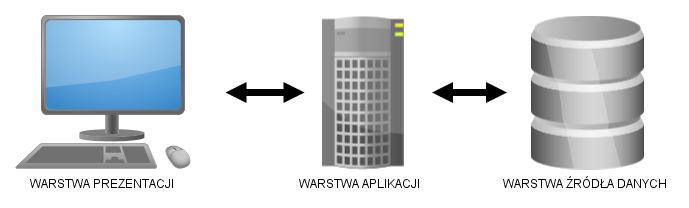
\includegraphics[scale=0.5]{../img/arch-3warstw.png}
    \end{center}
    \label{fig:arch3warstw}
    \caption{Schemat architektury trójwarstwowej}
\end{figure}
\FloatBarrier
W przypadku realizowanego systemu do obsługi magazynu zastosowana będzie
architektura trójwarstwowa.

%%%%%%%%%% DZIEDZINA PROBLEMU
\section{Dziedzina problemu}
Poniżej przedstawione zostały kluczowe pojęcia i procesy charakteryzujące system obsługi magazynu.

\subsection{Towary}
Towar jest podstawową jednostką przechowywaną w magazynie. Każdy towar jest opisany przez następujące cechy:
\begin{itemize}
	\item nazwa,
	\item kod kreskowy,
	\item kategoria,
	\item jednostka miary,
	\item stan początkowy (początkowa ilość towaru w magazynie),
	\item cena sprzedaży.
\end{itemize}

Możliwe są następujące operacje:
\begin{itemize}
	\item dodawanie towaru,
	\item edytowanie towaru z wyłączeniem bezpośredniej edycji stanu początkowego, który jest cechą ustalaną na podstawie dokumentów PZ, WZ oraz korekt magazynu,
	\item usuwanie towarów, które nie znajdują się w żadnym z dokumentów PZ, WZ lub korekcie magazynu.
\end{itemize}

Ponadto dla każdego towaru możliwe jest określenie stanu minimalnego oraz maksymalnego w magazynie, od którego zależna będzie możliwość dokonania operacji przyjęcia zamówienia, wydania zamówienia oraz korekty stanu magazynu.

\subsection{Dokumenty}
W systemie wyróżnione są trzy typy dokumentów: PZ, WZ oraz korekta stanu magazynu.

\subsubsection{PZ}
Dokument PZ jest dokumentem powiązanym z procesem przyjęcia towaru.
Dokument PZ zawiera:
\begin{itemize}
	\item numer dokumentu: PZnr\_kolejny\_dokumentu/rok, np: PZ1/2003,
	\item dane wystawcy (magazynu),
	\item dane kontrahenta,
	\item datę operacji,
	\item dane towarów wraz z ilością przyjętych towarów -- wartość ta dodaje się do stanu towaru w magazynie,
	\item cenę towaru, ustalaną indywidualnie dla każdego dokumentu PZ,
	\item łączną cenę towarów.
\end{itemize}

\subsubsection{WZ}
Dokument WZ jest dokumentem powiązanym z procesem wydania towaru.
Dokument WZ zawiera:
\begin{itemize}
	\item numer dokumentu: WZnr\_kolejny\_dokumentu/rok, np: WZ1/2003,
	\item dane wystawcy (magazynu),
	\item dane kontrahenta,
	\item datę operacji,
	\item dane towarów wraz z ilością przyjętych towarów -- wartość ta odejmuje się do stanu towaru w magazynie,
	\item cenę towaru, ustalaną indywidualnie dla każdego dokumentu WZ (cena towaru z danych towaru to tylko sugestia),
	\item łączną cenę towarów.
\end{itemize}

\subsubsection{Korekta stanu magazynu}
\begin{itemize}
	\item data korekty,
	\item numer dokumentu: Knr\_kolejny\_dokumentu/rok, np. K1/2013,
	\item dane towarów, których stan podlega korekcie,
	\item nowy stan towaru,
	\item suma modyfikowanej ilości towarów na dokumencie.
\end{itemize}

\subsubsection{Korekta PZ}
Korekta PZ jest dokumentem analogicznym do dokumentu PZ, z zastrzeżeniem, iż odnosi się ona do już istniejącego dokumentu PZ oraz dane z korekty PZ muszą być zgodne z danymi dokumentu PZ do którego ta korekta się odnosi -- w korekcie może znaleźć się tylko podzbiór towarów z dokumentu PZ a ilości poszczególnych towarów na korekcie nie mogą przekraczać ilości towarów oryginalnego dokumentu.

Ponadto:
\begin{itemize}
	\item numer dokumentu: PZknr\_kolejny\_dokumentu/rok, np PZk1/2013 (numer kolejny dokumentu nie jest w żaden sposób powiązany z jakimkolwiek numerem istniejącego dokumentu),
	\item cena towaru w korekcie PZ ustalana jest niezależnie od ceny z oryginalnego dokumentu PZ,
	\item ilość towaru w korekcie PZ odejmuje się od stanu towaru w magazynie.
\end{itemize}

\subsubsection{Korekta WZ}
Korekta WZ jest dokumentem analogicznym do dokumentu WZ, z zastrzeżeniem, iż odnosi się ona do już istniejącego dokumentu WZ oraz dane z korekty WZ muszą być zgodne z danymi dokumentu WZ do którego ta korekta się odnosi -- w korekcie może znaleźć się tylko podzbiór towarów z dokumentu WZ a ilości poszczególnych towarów na korekcie nie mogą przekraczać ilości towarów oryginalnego dokumentu.

Ponadto:
\begin{itemize}
	\item numer dokumentu: WZknr\_kolejny\_dokumentu/rok, np WZk1/2013 (numer kolejny dokumentu nie jest w żaden sposób powiązany z jakimkolwiek numerem istniejącego dokumentu),
	\item cena towaru w korekcie WZ ustalana jest niezależnie od ceny z oryginalnego dokumentu WZ,
	\item ilość towaru w korekcie WZ dodaje się od stanu towaru w magazynie.
\end{itemize}

\subsection{Przyjęcie towaru}
Z procesem przyjęcia towaru powiązane są następujące operacje:
\begin{itemize}
	\item utworzenie dokumentu PZ,
	\item edycja dokumentu PZ -- dowolne pole, zmiany ilości przyjętego towaru wpływają na stan towaru w magazynie,
	\item usunięcie dokumentu PZ -- usunięcie dokumentu PZ powoduje aktualizację (odjęcie) ilości towarów, które były uwzględnione w tym dokumencie.
\end{itemize}

\subsection{Wydanie towaru}
Z procesem wydania towaru powiązane są następujące operacje:
\begin{itemize}
	\item utworzenie dokumentu WZ,
	\item edycja dokumentu WZ -- dowolne pole, zmiany ilości przyjętego towaru wpływają na stan towaru w magazynie,
	\item usunięcie dokumentu WZ -- usunięcie dokumentu WZ powoduje aktualizację (dodanie) ilości towarów, które były uwzględnione w tym dokumencie.
\end{itemize}

Dodatkowo można wskazać przyjęcie towaru, do którego odnosi się to wydanie towaru: wtedy możliwe jest wskazanie wydawanego towaru, który był kiedyś przyjęty za pewną kwotę, a tym samym możliwe jest obliczenie zysku ze wydania towaru/wskazanie marży z towaru)

\section{Aktorzy}

Aktorzy w zaprojektowanym systemie zostali podzieleni na dwie grupy: aktorów
osobowych oraz aktorów nieosobowych. Do aktorów osobowym można zaliczyć
wszystkich użytkowników projektowanego systemu, aktorami nieosobowymi są
natomiast wszystkie systemy zewnętrzne współpracujące z projektowanym systemem.
Poniższy diagram przedstawia hierarchię aktorów osobowych w systemie:

\begin{figure}[h]
    \begin{center}
    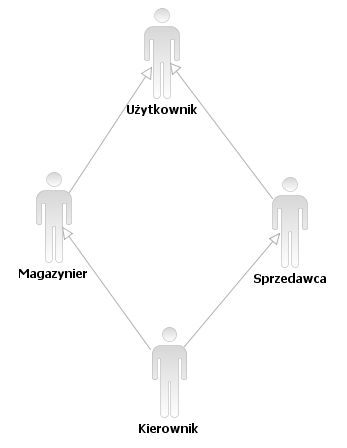
\includegraphics[scale=0.75]{../img/diagramDziedziczenia.png}
    \end{center}
    \label{fig:diagramDziedziczenia}
    \caption{Diagram przedstawiający aktorów w systemie}
\end{figure}
\FloatBarrier

\section{Wymagania funkcjonalne}

Niniejsze rozdział zawiera wymagania funkcjonalne jakie powinien spełniać
projektowany system. Wymagania te zostały podzielone na odpowiednie grupy wymagań.
Grupy wymagań zawierają bardziej szczegółowe wymagania, takie jak edycja czy
usuwanie danych. W tabeli umieszczone zostały również informacje o priorytecie
wymagania oraz ryzyku realizacji i aktorach.

%\arrayrulecolor{line}
%\rowcolors{2}{cell}{white}

\begin{table}[ht]
	 \begin{center}
% 	    \rowcolors{1}{}{light-blue}
	    \begin{tabular}{| l | l | l | l | l |}%\toprule
	    	\hline
		    \textbf{LP.} & \textbf{Nazwa}  & \textbf{Priorytet} & \textbf{Ryzyko} &
		    \textbf{Nazwa aktora} \\
		    \hline
			1 & Zarządzanie pracownikami & wysoki & niskie & kierownik \\
		    1.1 & Dodawanie pracownika & wysoki & niskie & kierownik \\
		    1.2 & Edycja danych pracownika & wysoki & niskie & kierownik \\ 	
		    1.3 & Usuwanie danych pracownika & wysoki &niskie & kierownik \\
		    \hline
		    2 & Zarządzanie danymi towarów & wysoki & niskie & magazynier \\
		    2.1 & Dodawanie towaru & wysoki &  niskie & magazynier \\
		    2.2 & Edycja opisu towaru & wysoki & niskie & magazynier \\
		    2.3 & Usuwanie danych towaru & wysoki & niskie & magazynier \\
            2.4 & Korekta stanu towaru & wysoki & niskie & magazynier \\
		    \hline
		   	3 & Zarządzanie danymi kontrahentów & wysoki & niskie & użytkownik \\
		   	3.1 & Dodawanie kontrahenta & wysoki & niski & użytkownik \\
		   	3.2 & Edycja danych kontrahenta & wysoki & niskie & użytkownik \\
		   	3.3 & Usuwanie danych kontrahenta & średni & niskie & użytkownik \\
		   	\hline
            4 & Przyjęcie na magazyn & wysoki & niskie & magazynier \\
		   	4.1 & Tworzenie dokumentu przejęcia towaru & wysoki & niskie & magazynier \\
		   	4.2 & Edycja dokumentu przyjęcia towaru & wysoki & niskie & magazynier \\
		   	4.3 & Usuwanie dokumentu przyjęcia towaru & wysoki & niskie & magazynier \\
		   	4.4 & Realizacja przyjęcia towaru & wysoki & niskie & magazynier \\
		   	4.5 & Korekta przyjęcia towaru & średni & niskie & magazynier \\
            \hline
		   	5 & Wydanie z magazynu & wysoki & niskie & sprzedawca \\
		   	5.1 & Tworzenie dokumentu wydania towaru & wysoki & niskie & sprzedawca \\
		   	5.2 & Edycja dokumentu wydania towaru & średni & niskie & sprzedawca \\
		   	5.3 & Usuwanie dokumentu wydania towaru & wysoki & niskie & sprzedawca \\
		   	5.4 & Realizacja wydania towaru & wysoki & niskie & sprzedawca \\
		   	5.5 & Korekta wydania towaru & średni & niskie & sprzedawca \\
		   	\hline
		   	6 & Zarządzanie raportami & średni & niskie & kierownik \\
		   	6.1 & Generowanie raportów o wydanych towarach & średni & niskie & kierownik \\
		   	6.2 & Generowanie raportów o przyjętych towarach & średni & niskie & kierownik \\
		   	\hline
	    \end{tabular}
	\end{center}
\end{table}
\FloatBarrier
\newpage

\section{Wymagania niefunkcjonalne}

Rozdział ten zawiera wymagania niefunkcjonalne dotyczące projektowanego systemu.
Wymagania zostały podzielone na kilka grup, przy każdym z wymagań został
określony priorytet oraz ryzyko.

\begin{table}[h]
	\begin{center}
		\begin{tabular}{| l | l | l | l |}
			\hline
			\textbf{Lp.} & \textbf{Nazwa} & \textbf{Priorytet} & \textbf{Ryzyko} \\
			\hline
			1 & Bezpieczeństwo & wysoki & niskie \\
			1.1 & Mechanizm uwierzytelniania użytkowników za pomocą & wysoki & niskie \\
			& loginu i hasła & & \\
			1.2 & Zróżnicowanie uprawnień do korzystania z systemu & wysoki & niskie \\
			1.3 & Zapisywanie historii przeprowadzanych transakcji & wysoki & niskie \\
			1.4 & Szyfrowanie haseł w bazie danych funkcją skrótu & wysoki & niskie \\
			\hline
			2 & Dostępność & wysoki & niskie \\
			2.1 & Dostępność systemu co najmniej 98\% w skali dnia & wysoki & niskie \\ 
			2.2 & Dostępność przez przeglądarkę & wysoki & niskie \\
			\hline
			3 & Elastyczność & wysoki & niskie \\
			3.1 & Architektura systemu umożliwia łatwą rozbudowę  & wysoki & niskie \\
			& i konserwacje & & \\
			3.2 & Możliwość integracji z innymi systemami używanymi & wysoki & niskie \\
			& w firmie & & \\
			
			\hline
			4 & Niezawodność & wysoki & niskie \\
			4.1 & Maksymalny czas powstania po awarii 2h & wysoki & niskie \\
			4.2 & Odtwarzanie uszkodzonych danych na podstawie & wysoki	& niskie \\
			& kopii zapasowych & & \\
			4.3 & Wykonywanie kopii zapasowych danych & wysoki & niskie \\
			\hline
			5 & Użyteczność & wysoki & niskie \\
			5.1 & Intuicyjny sposób obsługi systemy & wysoki & niskie \\
			5.2 & Przejrzysty system pomocy & wysoki & niskie \\
			\hline
			6 & Wydajność & wysoki & niskie \\
			6.1 & Przechowywanie informacji o transakcjach przez 3 lata & wysoki & niskie
			\\
			6.2 & Umożliwienie równoczesnej pracy przez 200 użytkowników & wysoki &
			niskie
			\\
			\hline
		\end{tabular}
	\end{center}
\end{table}
\FloatBarrier

\section{Dziedzina problemu}
Poniżej przedstawione zostały kluczowe pojęcia i procesy charakteryzujące system obsługi magazynu.

\subsection{Towary}
Towar jest podstawową jednostką przechowywaną w magazynie. Każdy towar jest opisany przez następujące cechy:
\begin{itemize}
	\item nazwa,
	\item kod kreskowy,
	\item kategoria,
	\item jednostka miary,
	\item stan początkowy (początkowa ilość towaru w magazynie),
	\item cena sprzedaży.
\end{itemize}

Możliwe są następujące operacje:
\begin{itemize}
	\item dodawanie towaru,
	\item edytowanie towaru z wyłączeniem bezpośredniej edycji stanu początkowego, który jest cechą ustalaną na podstawie dokumentów PZ, WZ oraz korekt magazynu,
	\item usuwanie towarów, które nie znajdują się w żadnym z dokumentów PZ, WZ lub korekcie magazynu.
\end{itemize}

Ponadto dla każdego towaru możliwe jest określenie stanu minimalnego oraz maksymalnego w magazynie, od którego zależna będzie możliwość dokonania operacji przyjęcia zamówienia, wydania zamówienia oraz korekty stanu magazynu.

\subsection{Dokumenty}
W systemie wyróżnione są trzy typy dokumentów: PZ, WZ oraz korekta stanu magazynu.

\subsubsection{PZ}
Dokument PZ jest dokumentem powiązanym z procesem przyjęcia towaru.
Dokument PZ zawiera:
\begin{itemize}
	\item numer dokumentu: PZnr\_kolejny\_dokumentu/rok, np: PZ1/2003,
	\item dane wystawcy (magazynu),
	\item dane kontrahenta,
	\item datę operacji,
	\item dane towarów wraz z ilością przyjętych towarów -- wartość ta dodaje się do stanu towaru w magazynie,
	\item cenę towaru, ustalaną indywidualnie dla każdego dokumentu PZ,
	\item łączną cenę towarów.
\end{itemize}

\subsubsection{WZ}
Dokument WZ jest dokumentem powiązanym z procesem wydania towaru.
Dokument WZ zawiera:
\begin{itemize}
	\item numer dokumentu: WZnr\_kolejny\_dokumentu/rok, np: WZ1/2003,
	\item dane wystawcy (magazynu),
	\item dane kontrahenta,
	\item datę operacji,
	\item dane towarów wraz z ilością przyjętych towarów -- wartość ta odejmuje się do stanu towaru w magazynie,
	\item cenę towaru, ustalaną indywidualnie dla każdego dokumentu WZ (cena towaru z danych towaru to tylko sugestia),
	\item łączną cenę towarów.
\end{itemize}

\subsubsection{Korekta stanu magazynu}
\begin{itemize}
	\item data korekty,
	\item numer dokumentu: Knr\_kolejny\_dokumentu/rok, np. K1/2013,
	\item dane towarów, których stan podlega korekcie,
	\item nowy stan towaru,
	\item suma modyfikowanej ilości towarów na dokumencie.
\end{itemize}

\subsubsection{Korekta PZ}
Korekta PZ jest dokumentem analogicznym do dokumentu PZ, z zastrzeżeniem, iż odnosi się ona do już istniejącego dokumentu PZ oraz dane z korekty PZ muszą być zgodne z danymi dokumentu PZ do którego ta korekta się odnosi -- w korekcie może znaleźć się tylko podzbiór towarów z dokumentu PZ a ilości poszczególnych towarów na korekcie nie mogą przekraczać ilości towarów oryginalnego dokumentu.

Ponadto:
\begin{itemize}
	\item numer dokumentu: PZknr\_kolejny\_dokumentu/rok, np PZk1/2013 (numer kolejny dokumentu nie jest w żaden sposób powiązany z jakimkolwiek numerem istniejącego dokumentu),
	\item cena towaru w korekcie PZ ustalana jest niezależnie od ceny z oryginalnego dokumentu PZ,
	\item ilość towaru w korekcie PZ odejmuje się od stanu towaru w magazynie.
\end{itemize}

\subsubsection{Korekta WZ}
Korekta WZ jest dokumentem analogicznym do dokumentu WZ, z zastrzeżeniem, iż odnosi się ona do już istniejącego dokumentu WZ oraz dane z korekty WZ muszą być zgodne z danymi dokumentu WZ do którego ta korekta się odnosi -- w korekcie może znaleźć się tylko podzbiór towarów z dokumentu WZ a ilości poszczególnych towarów na korekcie nie mogą przekraczać ilości towarów oryginalnego dokumentu.

Ponadto:
\begin{itemize}
	\item numer dokumentu: WZknr\_kolejny\_dokumentu/rok, np WZk1/2013 (numer kolejny dokumentu nie jest w żaden sposób powiązany z jakimkolwiek numerem istniejącego dokumentu),
	\item cena towaru w korekcie WZ ustalana jest niezależnie od ceny z oryginalnego dokumentu WZ,
	\item ilość towaru w korekcie WZ dodaje się od stanu towaru w magazynie.
\end{itemize}

\subsection{Przyjęcie towaru}
Z procesem przyjęcia towaru powiązane są następujące operacje:
\begin{itemize}
	\item utworzenie dokumentu PZ,
	\item edycja dokumentu PZ -- dowolne pole, zmiany ilości przyjętego towaru wpływają na stan towaru w magazynie,
	\item usunięcie dokumentu PZ -- usunięcie dokumentu PZ powoduje aktualizację (odjęcie) ilości towarów, które były uwzględnione w tym dokumencie.
\end{itemize}

\subsection{Wydanie towaru}
Z procesem wydania towaru powiązane są następujące operacje:
\begin{itemize}
	\item utworzenie dokumentu WZ,
	\item edycja dokumentu WZ -- dowolne pole, zmiany ilości przyjętego towaru wpływają na stan towaru w magazynie,
	\item usunięcie dokumentu WZ -- usunięcie dokumentu WZ powoduje aktualizację (dodanie) ilości towarów, które były uwzględnione w tym dokumencie.
\end{itemize}

Dodatkowo można wskazać przyjęcie towaru, do którego odnosi się to wydanie towaru: wtedy możliwe jest wskazanie wydawanego towaru, który był kiedyś przyjęty za pewną kwotę, a tym samym możliwe jest obliczenie zysku ze wydania towaru/wskazanie marży z towaru)
\chapter{Przypadki użycia}
\section{Moduł zarządzania systemem}
\singlespacing

\subsection{Zarządzanie pracownikami} 
Przypadek użycia umożliwiający zarządzanie pracownikami.
\begin{usecase}
% Pola na podstawie przykładowego szablonu z http://piotrsalata.pl/documents/wymagania.pdf.
% ID + nazwa
\addtitle{PU1}{Zarządzanie pracownikami} 
% Priorytet
\addfield{Priorytet:}{wysoki}
% Aktor główny - zazwyczaj ten, który inicjuje przypadek użycia.
\addfield{Aktor główny:}{Kierownik}
% Pozostali aktorzy uczestniczący 
%\additemizedfield{Aktorzy:}{
%	\item Sprzedawca
%	\item Magazynier
%}
% Warunki początkowe
\additemizedfield{Warunki początkowe:}{
  \item Aktor został uwierzytelniony.
} 
% Warunki końcowe
%\addfield{Warunki końcowe:} 
% Scenariusz główny
\addscenario{Scenariusz główny:}{
	\item Aktor wybiera opcję przeglądania pracowników.
    \item System wyświetla listę pracowników.
}
% Wyjątki
% \addfield{Wyjątki}{} TODO uwzględniać to?
% Wymagania funkcjonalne związane z danym przypadkiem użycia
\addfield{Wymagania funkcjonalne}{1. Zarządzanie pracownikami}
% Wymagania niefunkcjonalne - tylko gdy konieczne
% \addfield{Wymagania niefunkcjonalne}{}
\end{usecase}

\subsection{Dodawanie pracowników}
Przypadek użycia umożliwiający dodawanie pracowników.
\begin{usecase}
% Pola na podstawie przykładowego szablonu z http://piotrsalata.pl/documents/wymagania.pdf.
% ID + nazwa
\addtitle{PU2}{Dodawanie pracowników} 
% Priorytet
\addfield{Priorytet:}{wysoki}
% Aktor główny - zazwyczaj ten, który inicjuje przypadek użycia.
\addfield{Aktor główny:}{Kierownik}
% Pozostali aktorzy uczestniczący 
%\additemizedfield{Aktorzy:}{
%	\item Sprzedawca
%	\item Magazynier
%}
% Warunki początkowe
\additemizedfield{Warunki początkowe:}{
  \item Aktor został uwierzytelniony.
} 
% Warunki końcowe
\addfield{Warunki końcowe:}{Dane pracownika zostają zapisane w systemie}
% Scenariusz główny
\addscenario{Scenariusz główny:}{
	\item Aktor wybiera opcję dodania nowego pracownika.
    \item System wyświetla formularz umożliwiający wprowadzenie danych pracownika.
    \item Aktor wprowadza dane pracownika.
    \item Aktor zatwierdza wprowadzone dane.
    \item System sprawdza poprawność wprowadzonych danych.
    \item System zapisuje dane nowego pracownika.
    \item System wyświetla potwierdzenie wykonania operacji.
}
% Scenariusze alternatywne
\addscenario{Scenariusz alternatywny:}{
  % [nr kroku scenariusza głównego.kolejna litera a,b,c wyznaczająca kolejny scenariusz alternatywny od wybranego kroku s.głównego.
	\item[6.a] Wprowadzono błędne dane
		\begin{enumerate}
		\item[1.--5.] Jak w scenariuszu głównym.
		\item[6.] System wyświetla komunikat informujący o wprowadzeniu błędnych danych.
		\item[7.] Powrót do punktu 3. scenariusza głównego.
		\end{enumerate}
}
% Wyjątki
% \addfield{Wyjątki}{} TODO uwzględniać to?
% Wymagania funkcjonalne związane z danym przypadkiem użycia
\addfield{Wymagania funkcjonalne}{1. Zarządzanie pracownikami}
% Wymagania niefunkcjonalne - tylko gdy konieczne
% \addfield{Wymagania niefunkcjonalne}{}
\end{usecase}

\subsection{Edycja danych pracowników}
Przypadek użycia opisujący edycję danych pracowników.
\begin{usecase}
% Pola na podstawie przykładowego szablonu z http://piotrsalata.pl/documents/wymagania.pdf.
% ID + nazwa
\addtitle{PU3}{Edycja danych pracowników} 
% Priorytet
\addfield{Priorytet:}{wysoki}
% Aktor główny - zazwyczaj ten, który inicjuje przypadek użycia.
\addfield{Aktor główny:}{Kierownik}
% Pozostali aktorzy uczestniczący 
%\additemizedfield{Aktorzy:}{
%	\item Sprzedawca
%	\item Magazynier
%}
% Warunki początkowe
\additemizedfield{Warunki początkowe:}{
  \item Aktor został uwierzytelniony.
  \item W systemie istnieje co najmniej jeden pracownik.
} 
% Warunki końcowe
\addfield{Warunki końcowe:}{Dane pracownika zostają zmienione w systemie}
% Scenariusz główny
\addscenario{Scenariusz główny:}{
	\item Aktor wybiera opcję edycji pracownika.
    \item System wyświetla formularz umożliwiający modyfikację danych pracownika.
    \item Aktor modyfikuje dane pracownika.
    \item Aktor zatwierdza wprowadzone zmiany.
    \item System sprawdza poprawność wprowadzonych danych.
    \item System zapisuje zmienione dane pracownika.
    \item System wyświetla potwierdzenie wykonania operacji.
}
% Scenariusze alternatywne
\addscenario{Scenariusz alternatywny:}{
  % [nr kroku scenariusza głównego.kolejna litera a,b,c wyznaczająca kolejny scenariusz alternatywny od wybranego kroku s.głównego.
	\item[6.a] Wprowadzono błędne dane
		\begin{enumerate}
		\item[1.--5.] Jak w scenariuszu głównym.
		\item[6.] System wyświetla komunikat informujący o wprowadzeniu błędnych danych.
		\item[7.] Powrót do punktu 3. scenariusza głównego.
		\end{enumerate}
}
% Wyjątki
% \addfield{Wyjątki}{} TODO uwzględniać to?
% Wymagania funkcjonalne związane z danym przypadkiem użycia
\addfield{Wymagania funkcjonalne}{1. Zarządzanie pracownikami}
% Wymagania niefunkcjonalne - tylko gdy konieczne
% \addfield{Wymagania niefunkcjonalne}{}
\end{usecase}

\subsection{Usuwanie danych pracowników}
Przypadek użycia opisujący usuwanie danych pracowników.
\begin{usecase}
% Pola na podstawie przykładowego szablonu z http://piotrsalata.pl/documents/wymagania.pdf.
% ID + nazwa
\addtitle{PU4}{Usuwanie danych pracowników} 
% Priorytet
\addfield{Priorytet:}{wysoki}
% Aktor główny - zazwyczaj ten, który inicjuje przypadek użycia.
\addfield{Aktor główny:}{Kierownik}
% Pozostali aktorzy uczestniczący 
%\additemizedfield{Aktorzy:}{
%	\item Sprzedawca
%	\item Magazynier
%}
% Warunki początkowe
\additemizedfield{Warunki początkowe:}{
  \item Aktor został uwierzytelniony.
  \item W istnieje co najmniej jeden pracownik.
} 
% Warunki końcowe
\addfield{Warunki końcowe:}{Dane pracownika zostają usunięte z systemu.}
% Scenariusz główny
\addscenario{Scenariusz główny:}{
	\item Aktor wybiera opcję usunięcia pracownika.
    \item System wyświetla okno potwierdzenia.
    \item Aktor zatwierdza usunięcie pracownika.
    \item System usuwa dane pracownika.
    \item System wyświetla potwierdzenie wykonania operacji.
}
% Scenariusze alternatywne
\addscenario{Scenariusz alternatywny:}{
  % [nr kroku scenariusza głównego.kolejna litera a,b,c wyznaczająca kolejny scenariusz alternatywny od wybranego kroku s.głównego.
	\item[3.a] Aktor anuluje usuwanie pracownika
		\begin{enumerate}
		\item[1.--2.] Jak w scenariuszu głównym.
		\item[3.] System zamyka okno potwierdzenia.
		\end{enumerate}
}
% Wyjątki
% \addfield{Wyjątki}{} TODO uwzględniać to?
% Wymagania funkcjonalne związane z danym przypadkiem użycia
\addfield{Wymagania funkcjonalne}{1. Zarządzanie pracownikami}
% Wymagania niefunkcjonalne - tylko gdy konieczne
% \addfield{Wymagania niefunkcjonalne}{}
\end{usecase}

\subsection{Zarządzanie raportami} 
Przypadek użycia umożliwiający zarządzanie raportami.
\begin{usecase}
% Pola na podstawie przykładowego szablonu z http://piotrsalata.pl/documents/wymagania.pdf.
% ID + nazwa
\addtitle{PU5}{Zarządzanie raportami} 
% Priorytet
\addfield{Priorytet:}{średni}
% Aktor główny - zazwyczaj ten, który inicjuje przypadek użycia.
\addfield{Aktor główny:}{Kierownik}
% Pozostali aktorzy uczestniczący 
%\additemizedfield{Aktorzy:}{
%	\item Sprzedawca
%	\item Magazynier
%}
% Warunki początkowe
\additemizedfield{Warunki początkowe:}{
  \item Aktor został uwierzytelniony.
  \item W systemie przechowywana jest informacja o co najmniej jednej sprzedaży/zakupie.
} 
% Warunki końcowe
%\addfield{Warunki końcowe: } 
% Scenariusz główny
\addscenario{Scenariusz główny:}{
	\item Aktor wybiera opcję tworzenia raportów.
    \item System wyświetla listę możliwych dostępnych typów raportów.
}
% Wyjątki
% \addfield{Wyjątki}{} TODO uwzględniać to?
% Wymagania funkcjonalne związane z danym przypadkiem użycia
\addfield{Wymagania funkcjonalne}{7. Zarządzanie raportami}
% Wymagania niefunkcjonalne - tylko gdy konieczne
% \addfield{Wymagania niefunkcjonalne}{}
\end{usecase}

\subsection{Generowanie raportów sprzedaży}
Przypadek użycia umożliwiający generowanie raportów sprzedaży.
\begin{usecase}
% Pola na podstawie przykładowego szablonu z http://piotrsalata.pl/documents/wymagania.pdf.
% ID + nazwa
\addtitle{PU6}{Generowanie raportów sprzedaży} 
% Priorytet
\addfield{Priorytet:}{średni}
% Aktor główny - zazwyczaj ten, który inicjuje przypadek użycia.
\addfield{Aktor główny:}{Kierownik}
% Pozostali aktorzy uczestniczący 
%\additemizedfield{Aktorzy:}{
%	\item Sprzedawca
%	\item Magazynier
%}
% Warunki początkowe
\additemizedfield{Warunki początkowe:}{
  \item Aktor został uwierzytelniony.
  \item W systemie przechowywana jest informacja o co najmniej jednej sprzedaży.
} 
% Warunki końcowe
\addfield{Warunki końcowe:} {Aktor posiada dokument z raportem sprzedaży.} 
% Scenariusz główny
\addscenario{Scenariusz główny:}{
	\item Aktor wybiera opcję dodania generowania raportu sprzedaży.
    \item System generuje raport sprzedaży.
}
% Scenariusze alternatywne
%\addscenario{Przebiegi alternatywne:}{
  % [nr kroku scenariusza głównego.kolejna litera a,b,c wyznaczająca kolejny scenariusz alternatywny od wybranego kroku s.głównego.
%}
% Wyjątki
% \addfield{Wyjątki}{} TODO uwzględniać to?
% Wymagania funkcjonalne związane z danym przypadkiem użycia
\addfield{Wymagania funkcjonalne}{7. Zarządzanie raportami}
% Wymagania niefunkcjonalne - tylko gdy konieczne
% \addfield{Wymagania niefunkcjonalne}{}
\end{usecase}
\section{Moduł obsługi kontrahentów}
\singlespacing

\subsection{Zarządzanie danymi kontrahentów} 
\begin{usecase}
\addtitle{PU8}{Zarządzanie danymi kontrahentów} 
% Priorytet
\addfield{Priorytet:}{wysoki}
\addfield{Aktor główny:}{Użytkownik}
\additemizedfield{Warunki początkowe:}{
  \item Aktor został uwierzytelniony.
} 
\addscenario{Scenariusz główny:}{
	\item Aktor wybiera opcję przeglądania kontrahentów.
    \item System wyświetla listę kontrahentów.
}
\addfield{Wymagania funkcjonalne}{3. Zarządzanie danymi kontrahentów}
\end{usecase}

\begin{figure}[H]
  \centering
  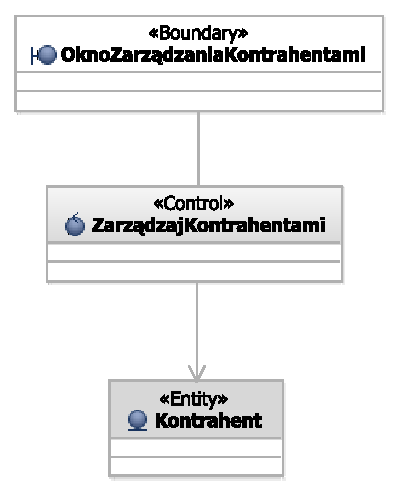
\includegraphics[angle=\ecbangle, scale=\ecbscale]{../img/usecase/pu8ecb.pdf}
  \caption{\ecbcaption8}
\end{figure}
\newpage %!!!!!!!!!!!!!!!!!!!!! RECZNA zmiana strony!
\begin{figure}[H]
  \centering
  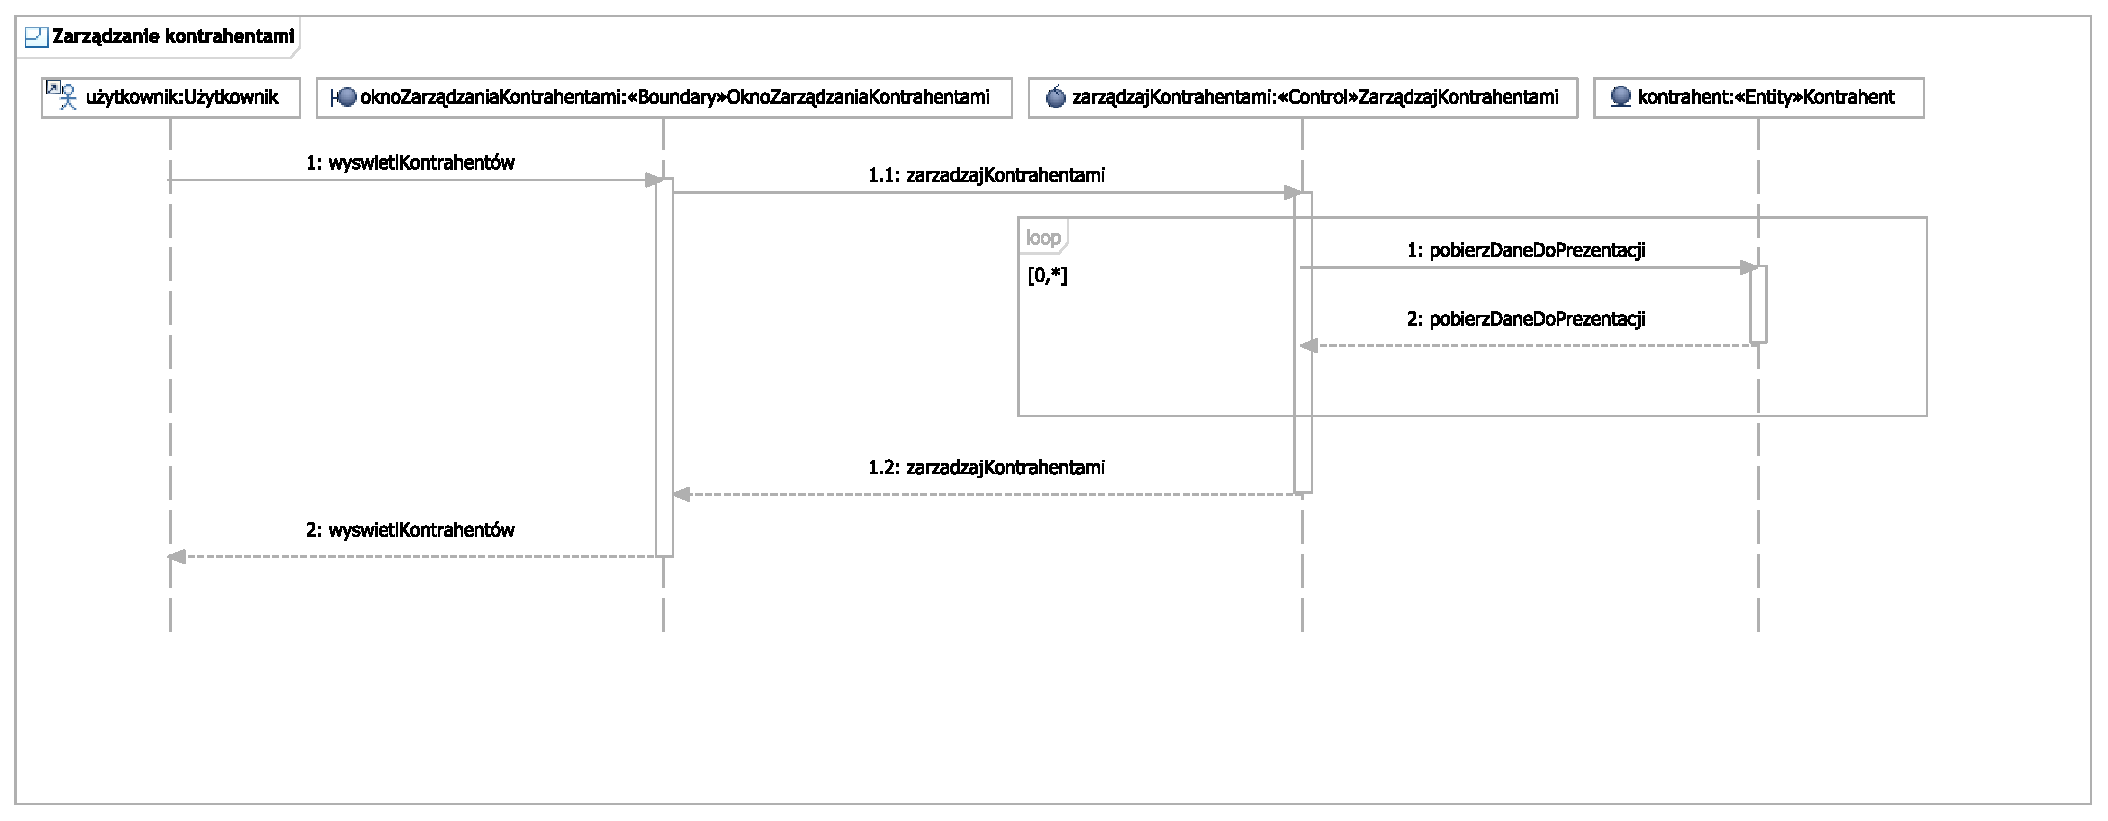
\includegraphics[angle=\seqangle, scale=0.45]{../img/usecase/pu8seq.pdf}
  \caption{\seqcaption8}
\end{figure}
\newpage

\subsection{Dodawanie kontrahentów}
\begin{usecase}
\addtitle{PU9}{Dodawanie kontrahenta} 
\addfield{Priorytet:}{wysoki}
\addfield{Aktor główny:}{Użytkownik}
\addfield{Rozszerza przypadki:}{PU8}
\additemizedfield{Warunki początkowe:}{
  \item Aktor został uwierzytelniony.
} 
\addfield{Warunki końcowe:}{Dane kontrahenta zostają zapisane w systemie}
\addscenario{Scenariusz główny:}{
	\item Aktor wybiera opcję dodania nowego kontrahenta.
    \item System wyświetla formularz umożliwiający wprowadzenie danych kontrahenta.
    \item Aktor wprowadza dane kontrahenta.
    \item Aktor zatwierdza wprowadzone dane.
    \item System sprawdza poprawność wprowadzonych danych.
    \item System zapisuje dane nowego kontrahenta.
    \item System wyświetla potwierdzenie wykonania operacji.
}
\addscenario{Scenariusz alternatywny:}{
	\item[6.a] Wprowadzono błędne dane
		\begin{enumerate}
		\item[1.--5.] Jak w scenariuszu głównym.
		\item[6.] System wyświetla komunikat informujący o wprowadzeniu błędnych danych.
		\item[7.] Powrót do punktu 3. scenariusza głównego.
		\end{enumerate}
}
\addfield{Wymagania funkcjonalne}{3. Zarządzanie danymi kontrahentów, 3.1 Dodawanie kontrahentów}
\end{usecase}

\begin{figure}[H]
  \centering
  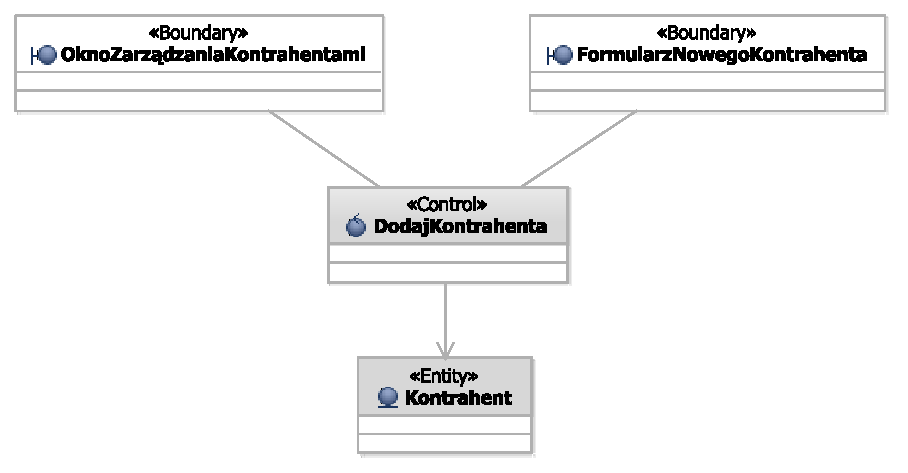
\includegraphics[angle=\ecbangle, scale=\ecbscale]{../img/usecase/pu9ecb.pdf}
  \caption{\ecbcaption9}
\end{figure}
\begin{figure}[H]
  \centering
  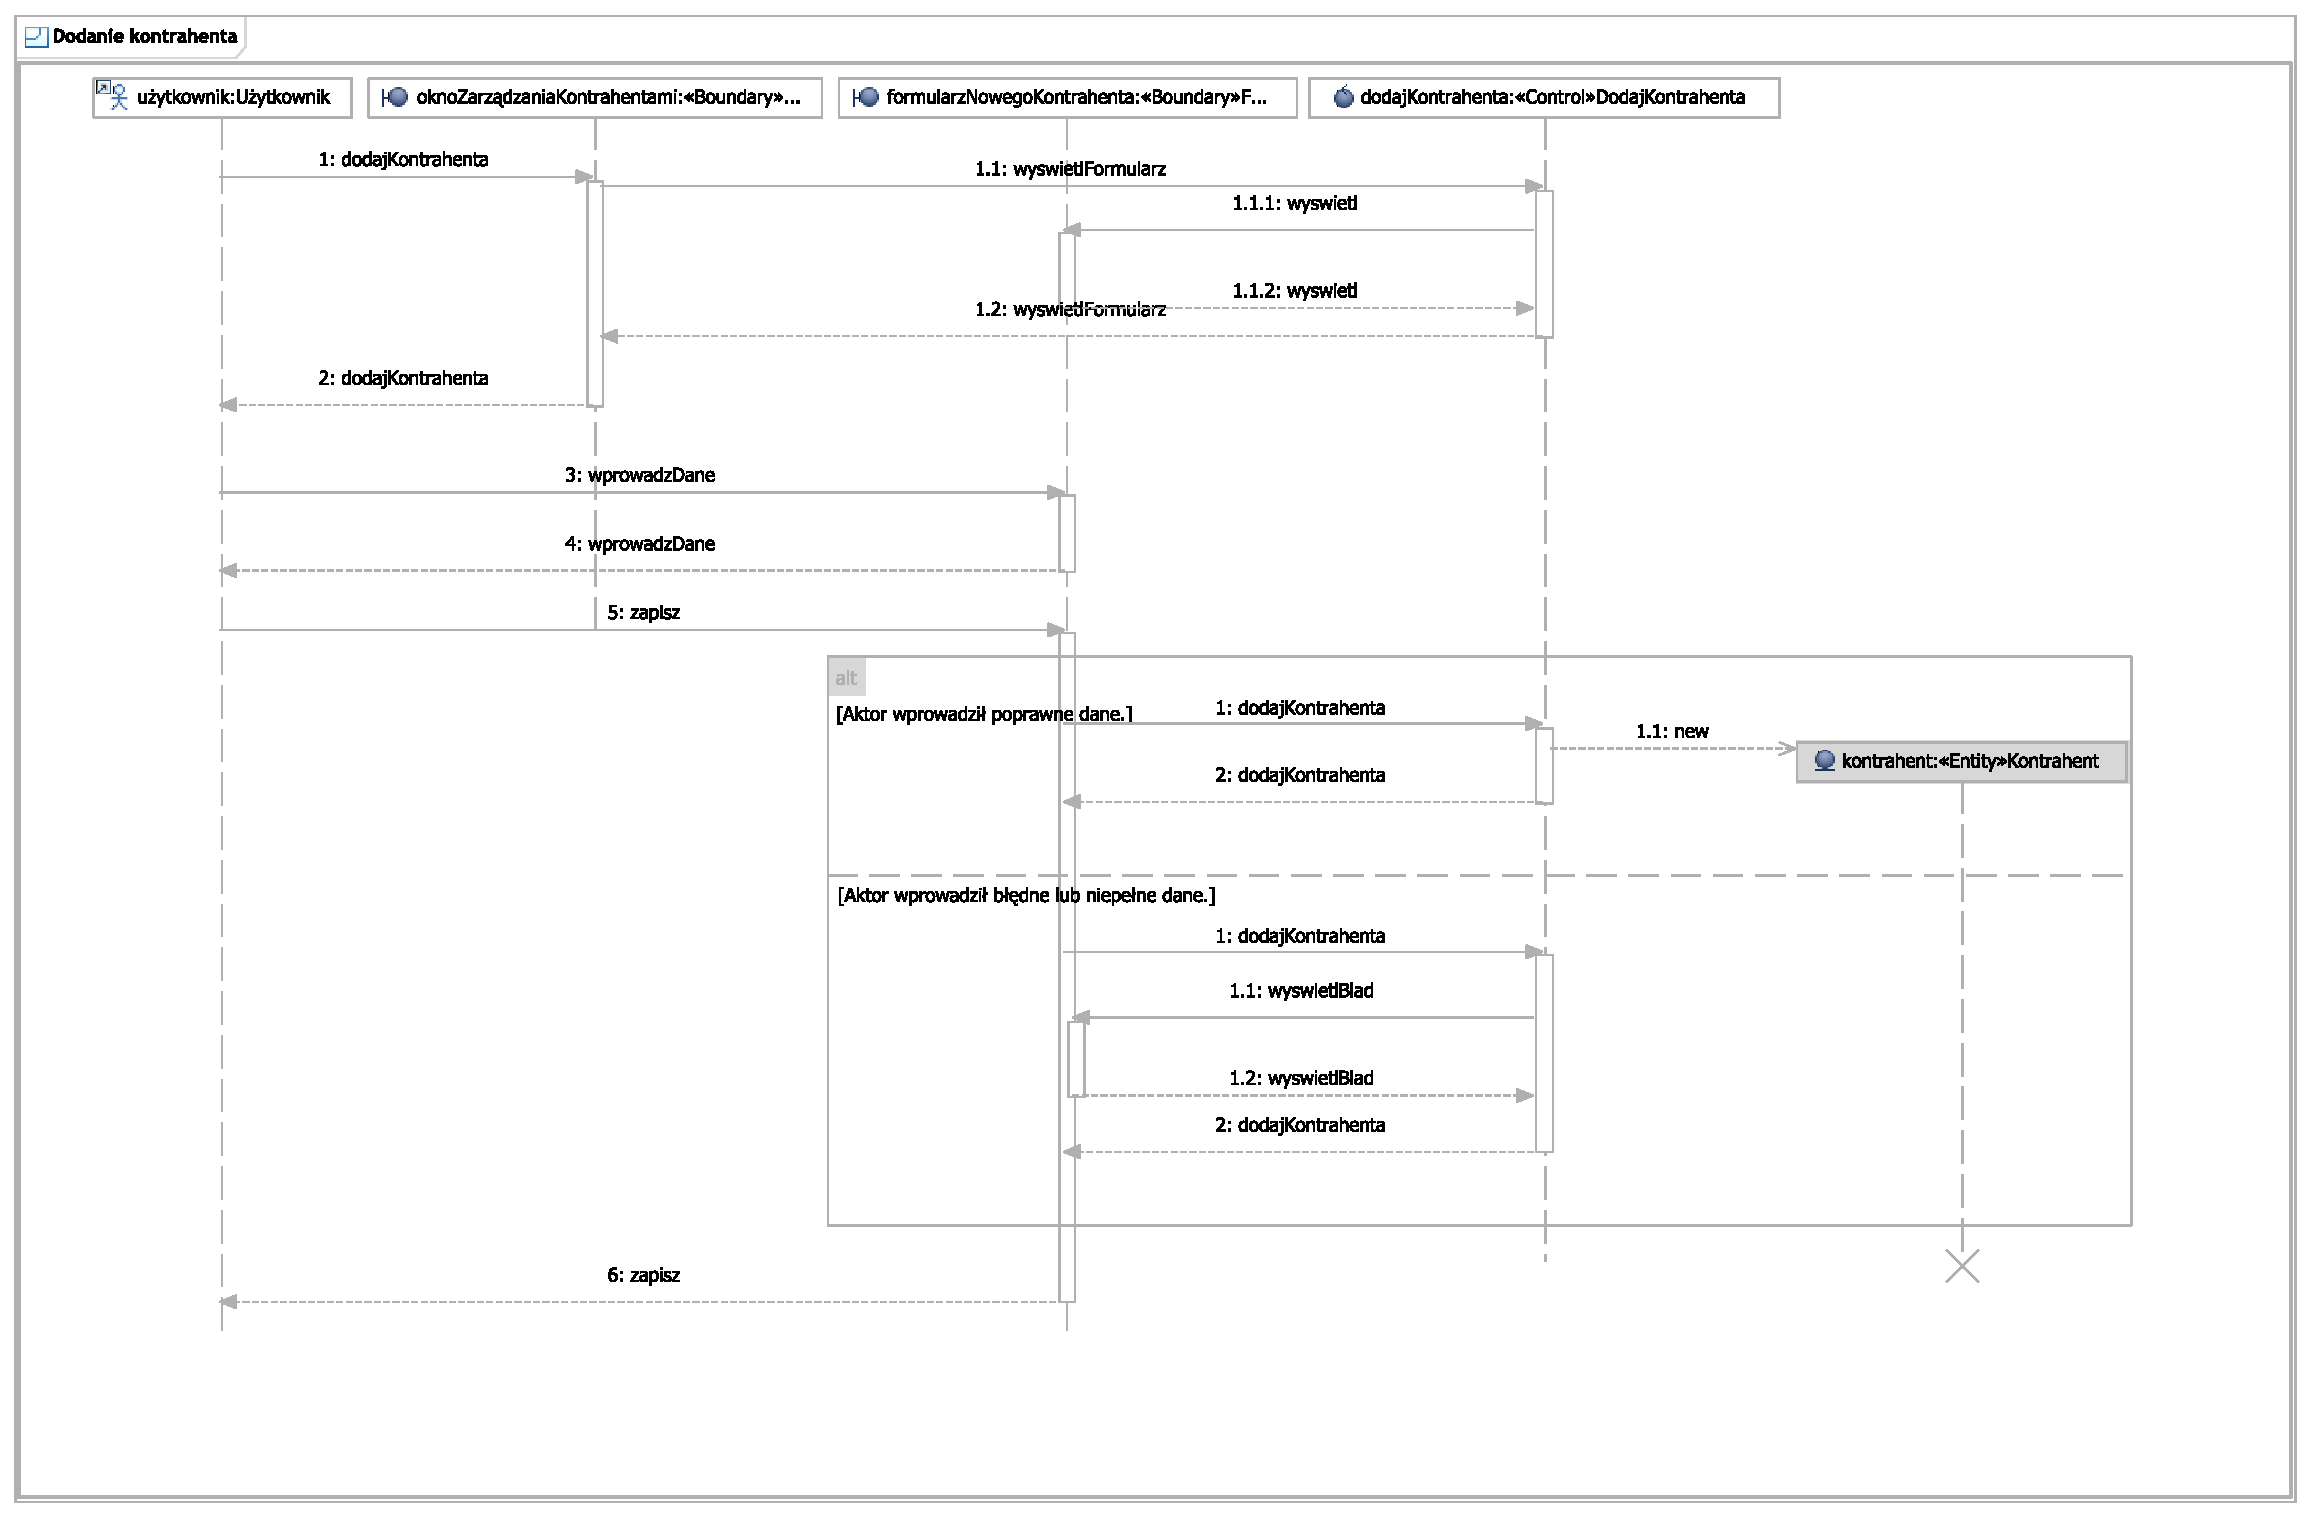
\includegraphics[angle=\seqangle, scale=\seqscalemin]{../img/usecase/pu9seq.pdf}
  \caption{\seqcaption9}
\end{figure}
\newpage

\subsection{Edycja danych kontrahentów}
\begin{usecase}
\addtitle{PU10}{Edycja danych kontrahenta} 
\addfield{Priorytet:}{wysoki}
\addfield{Aktor główny:}{Użytkownik}
\addfield{Rozszerza przypadki:}{PU8}
\additemizedfield{Warunki początkowe:}{
  \item Aktor został uwierzytelniony.
  \item W systemie istnieje co najmniej jeden kontrahent.
} 
\addfield{Warunki końcowe:}{Dane kontrahenta zostają zmienione w systemie}
\addscenario{Scenariusz główny:}{
	\item Aktor wybiera opcję edycji kontrahenta.
    \item System wyświetla formularz umożliwiający modyfikację danych kontrahenta.
    \item Aktor modyfikuje dane kontrahenta.
    \item Aktor zatwierdza wprowadzone zmiany.
    \item System sprawdza poprawność wprowadzonych danych.
    \item System zapisuje zmienione dane kontrahenta.
    \item System wyświetla potwierdzenie wykonania operacji.
}
\addscenario{Scenariusz alternatywny:}{
	\item[6.a] Wprowadzono błędne dane
		\begin{enumerate}
		\item[1.--5.] Jak w scenariuszu głównym.
		\item[6.] System wyświetla komunikat informujący o wprowadzeniu błędnych danych.
		\item[7.] Powrót do punktu 3. scenariusza głównego.
		\end{enumerate}
}
\addfield{Wymagania funkcjonalne}{3. Zarządzanie danymi kontrahentów, 3.2 Edycja danych kontrahentów}
\end{usecase}

\begin{figure}[H]
  \centering
  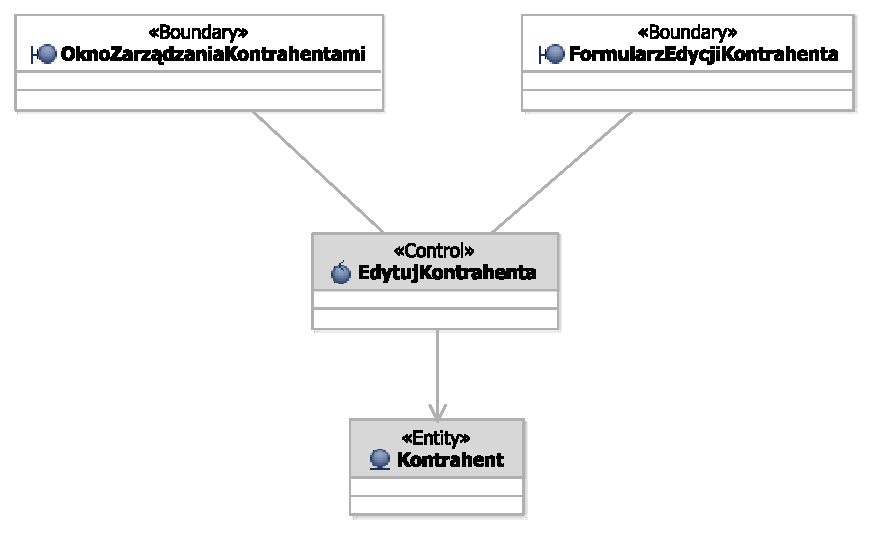
\includegraphics[angle=\ecbangle, scale=\ecbscale]{../img/usecase/pu10ecb.pdf}
  \caption{\ecbcaption10}
\end{figure}
\begin{figure}[H]
  \centering
  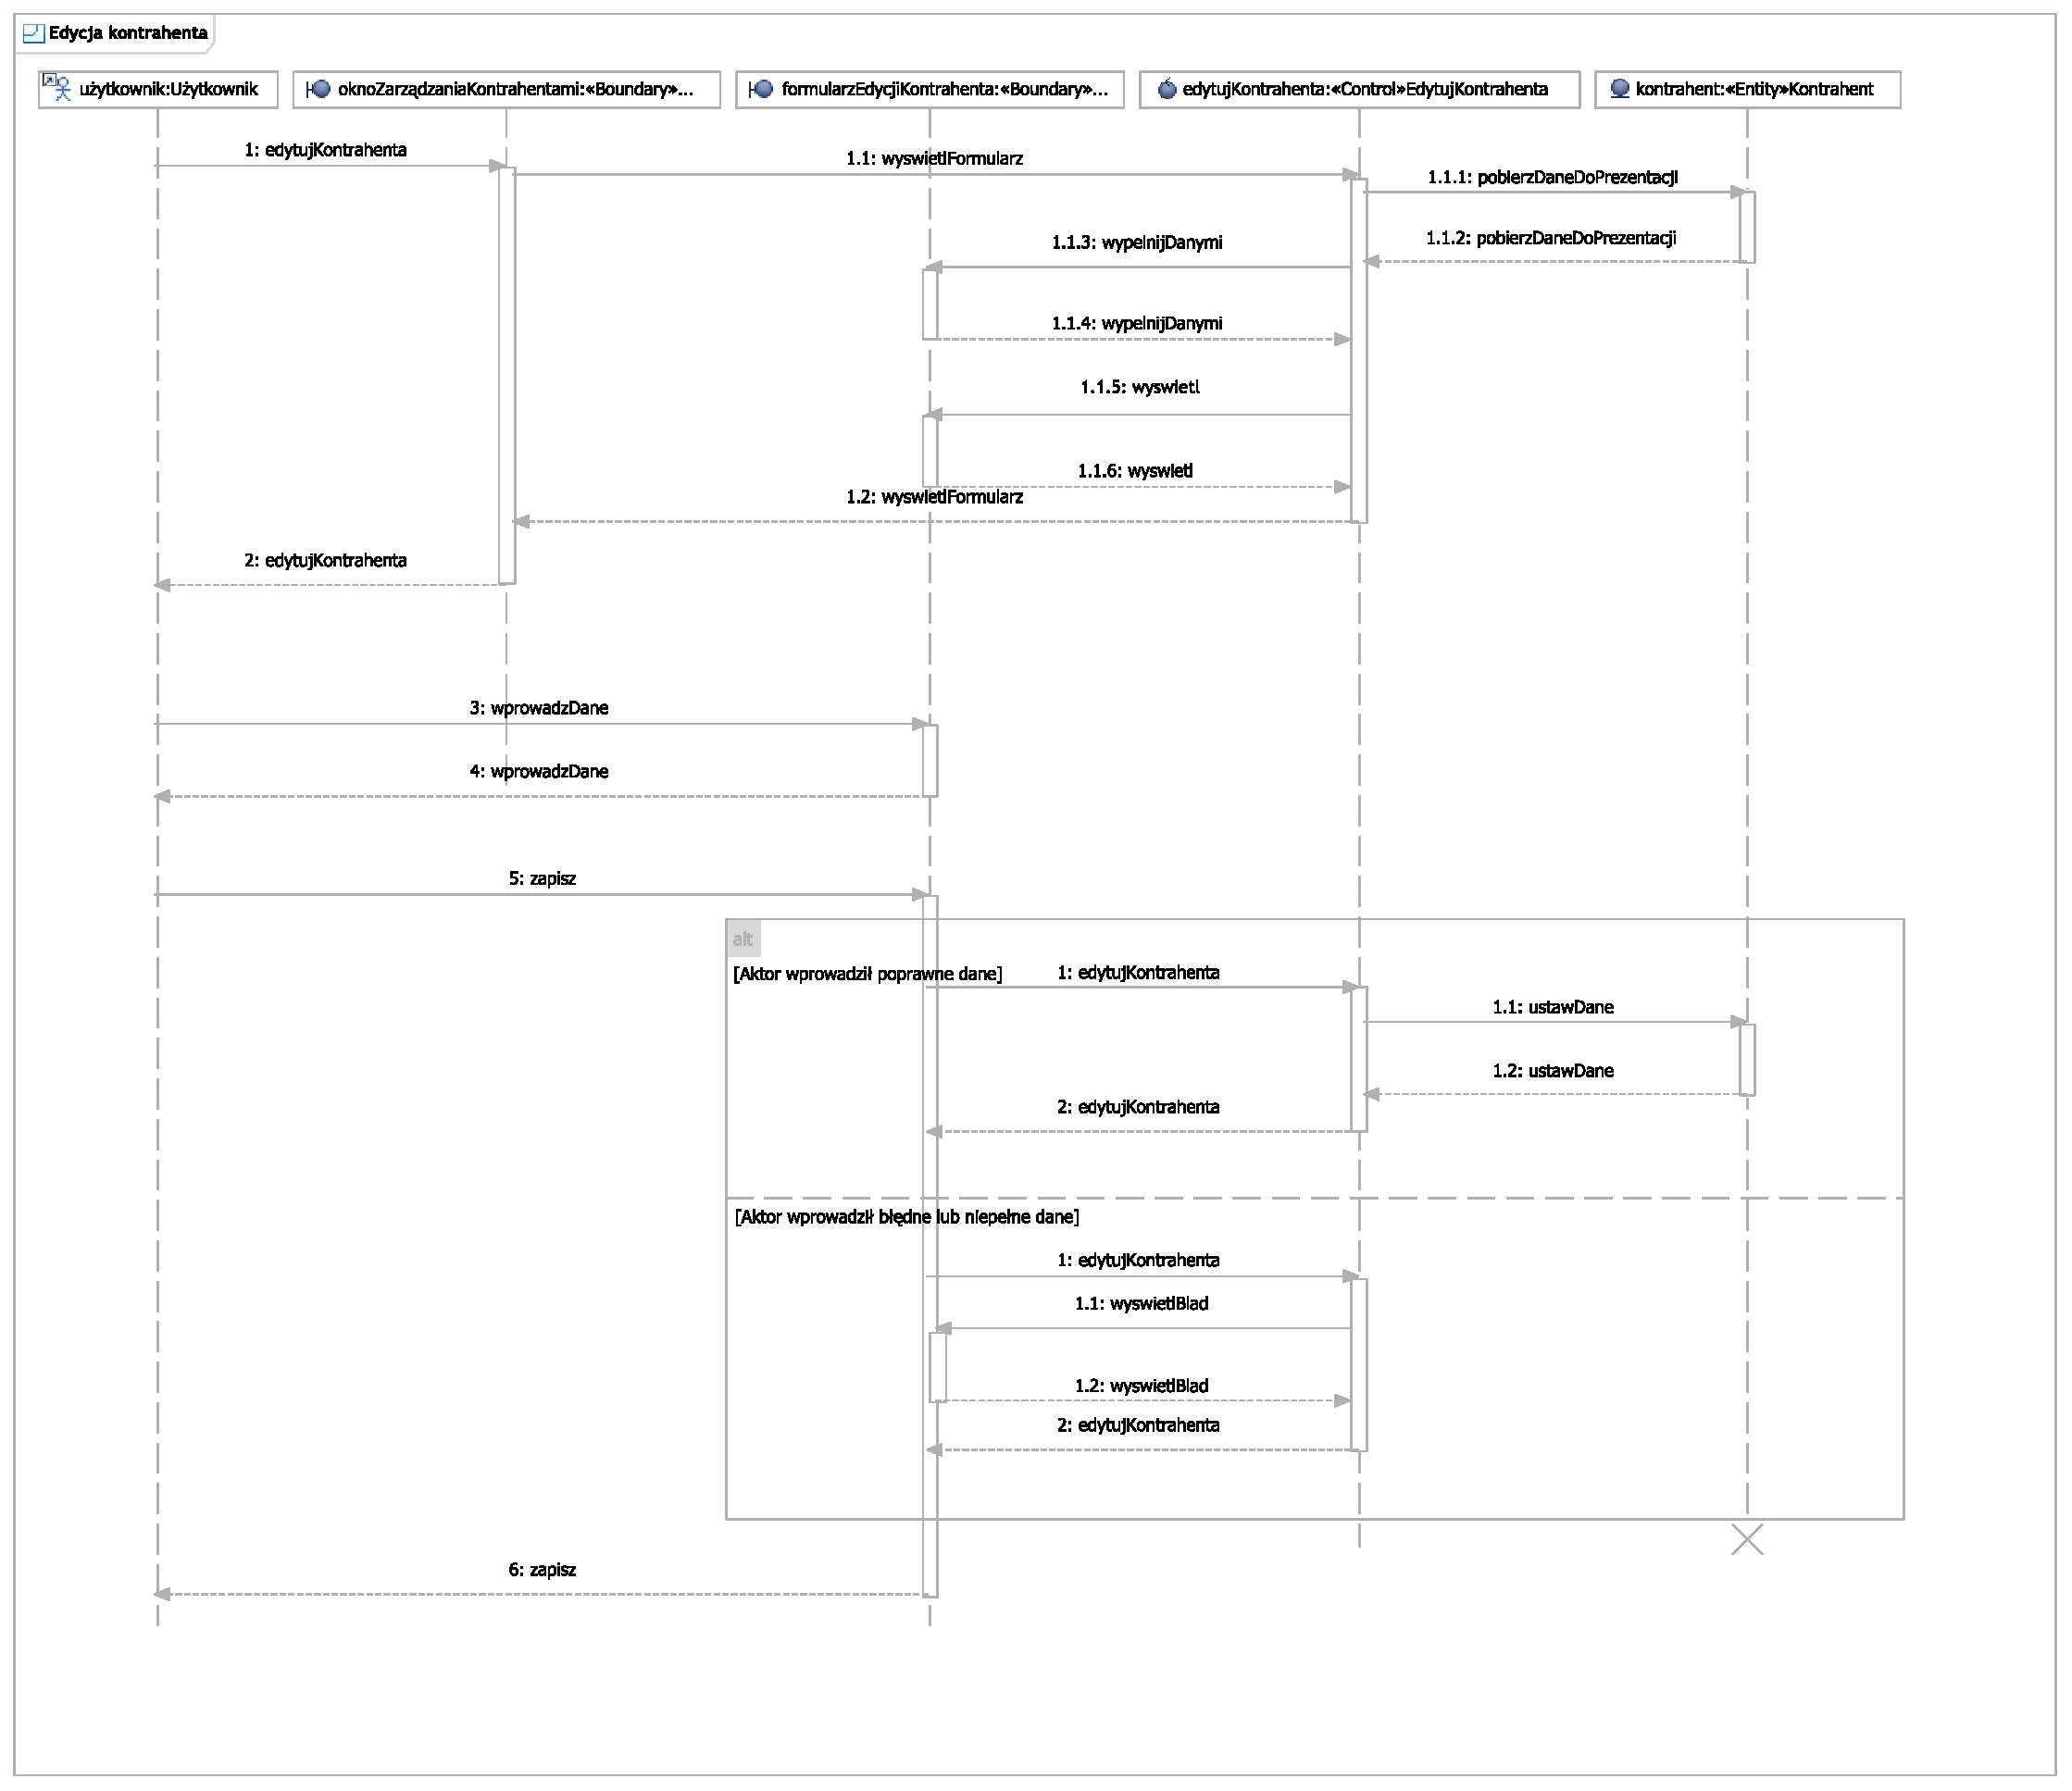
\includegraphics[angle=\seqangle, scale=0.43]{../img/usecase/pu10seq.pdf}
  \caption{\seqcaption10}
\end{figure}
\newpage

\subsection{Usuwanie danych kontrahentów}
\begin{usecase}
\addtitle{PU11}{Usuwanie danych kontrahenta} 
\addfield{Priorytet:}{wysoki}
\addfield{Aktor główny:}{Użytkownik}
\addfield{Rozszerza przypadki:}{PU8}
\additemizedfield{Warunki początkowe:}{
  \item Aktor został uwierzytelniony.
  \item W istnieje co najmniej jeden kontrahent.
} 
\addfield{Warunki końcowe:}{Dane kontrahenta zostają usunięte z systemu.}
\addscenario{Scenariusz główny:}{
	\item Aktor wybiera opcję usunięcia kontrahenta.
    \item System wyświetla okno potwierdzenia.
    \item Aktor zatwierdza usunięcie kontrahenta.
    \item System usuwa dane kontrahenta.
    \item System wyświetla potwierdzenie wykonania operacji.
}
\addscenario{Scenariusz alternatywny:}{
	\item[3.a] Aktor anuluje usuwanie kontrahenta.
		\begin{enumerate}
		\item[1.--2.] Jak w scenariuszu głównym.
		\item[3.] System zamyka okno potwierdzenia.
		\end{enumerate}
}
\addfield{Wymagania funkcjonalne}{3. Zarządzanie danymi kontrahentów, 3.3 Usuwanie danych kontrahentów}
\end{usecase}

\begin{figure}[H]
  \centering
  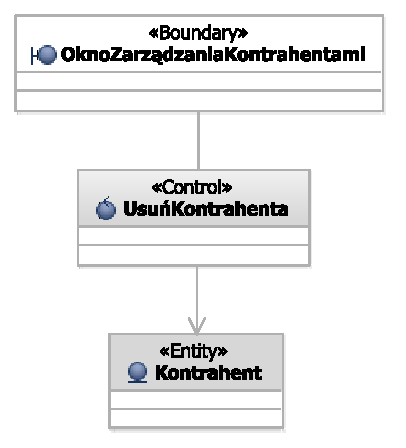
\includegraphics[angle=\ecbangle, scale=\ecbscale]{../img/usecase/pu11ecb.pdf}
  \caption{\ecbcaption11}
\end{figure}
\begin{figure}[H]
  \centering
  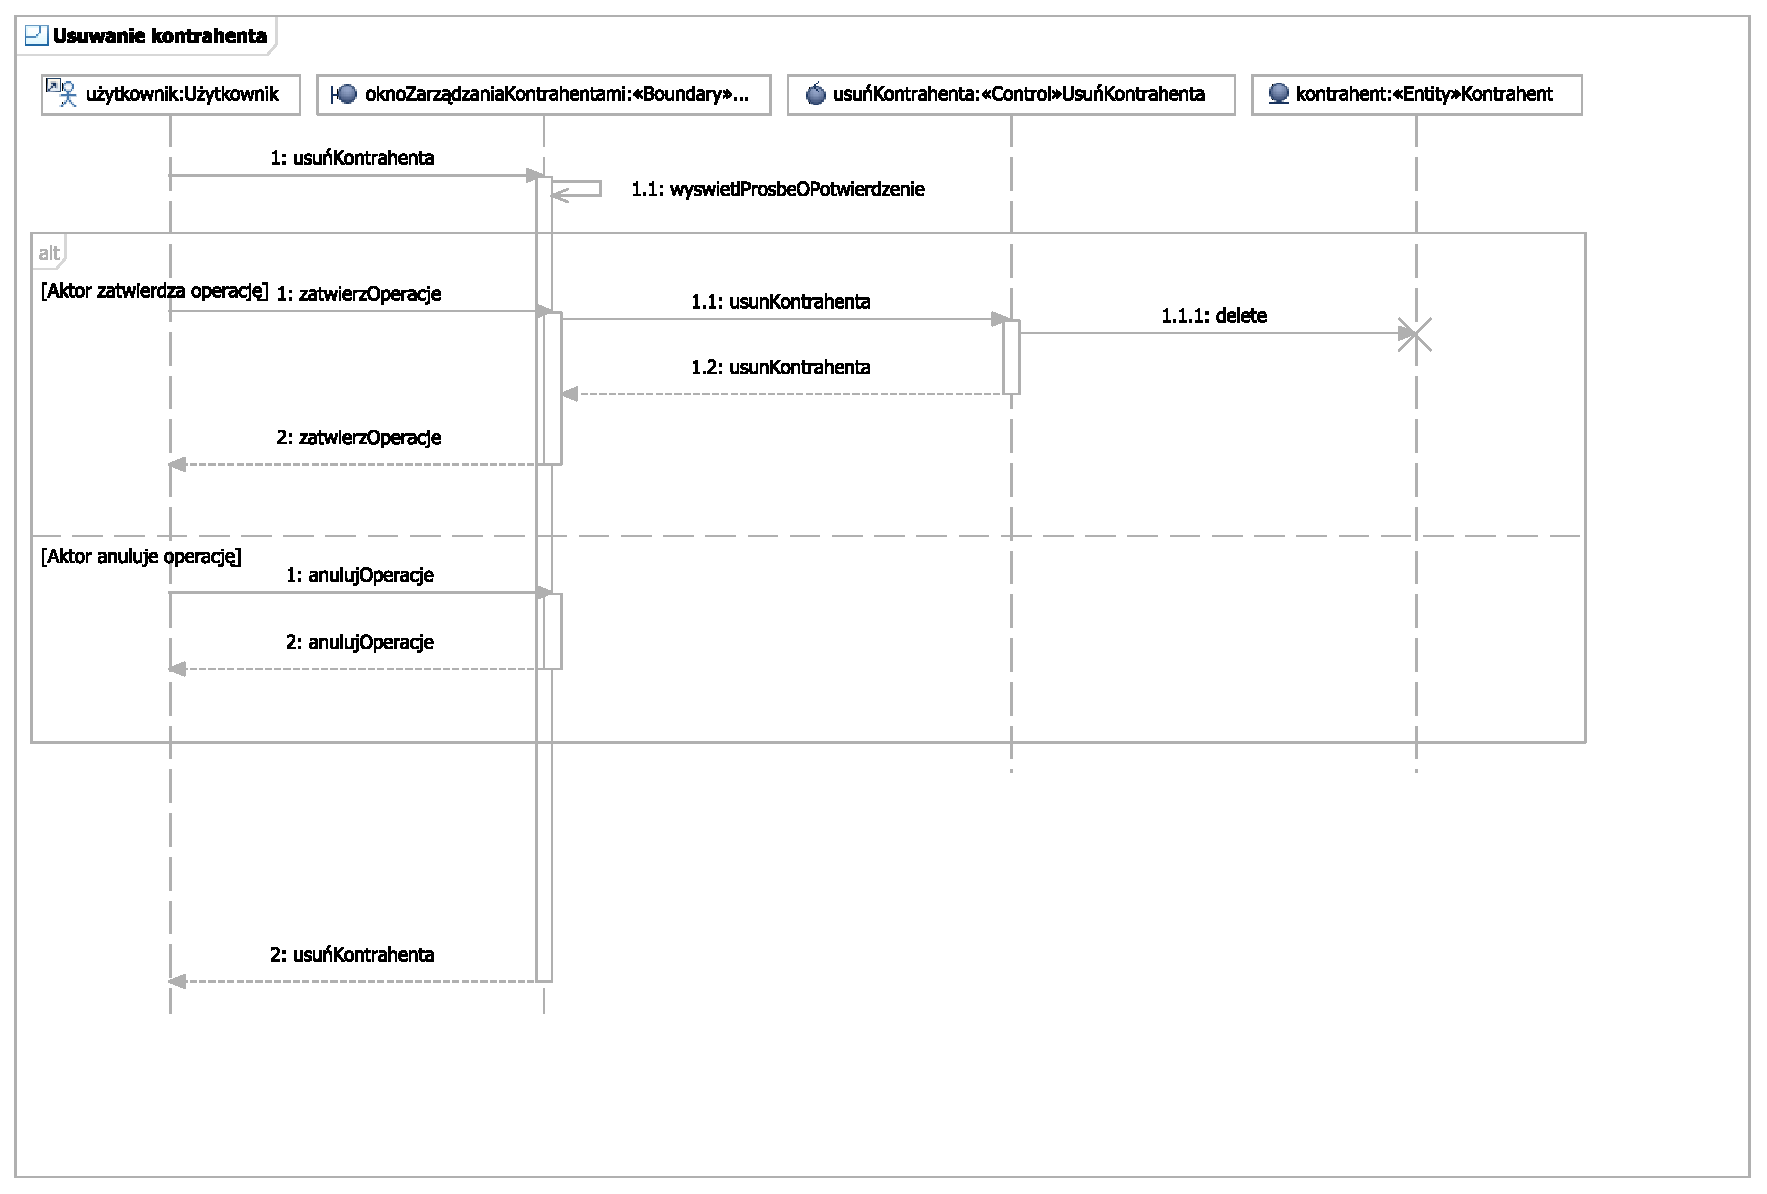
\includegraphics[angle=\seqangle, scale=0.55]{../img/usecase/pu11seq.pdf}
  \caption{\seqcaption11}
\end{figure}
\newpage

\section{Sprzedaż}
Sprzedawca pośredniczy w kontaktach z kontrahentem i zarządza procesem
sprzedaży towarów. Przyjmuje on zamówienia (wykonuje operacje wydania
towaru z magazynu) i dodaje je do bazy, aktualizując jednocześnie dane
klientów. Sprawuje kontrolę nad realizacją wydania towaru z magazynu,
a w razie potrzeby może przyjąć zwrócony towar. Do zadań sprzedawcy
należy prowadzenie ewidencji kontrahentów, aktualizowanie informacji o
nich oraz usuwanie starych. Przypadki użycia sprzedawcy zostały
zaprezentowane na diagramie \ref{fig:Sprzedaz}.

\begin{figure}[H]
  \centering
  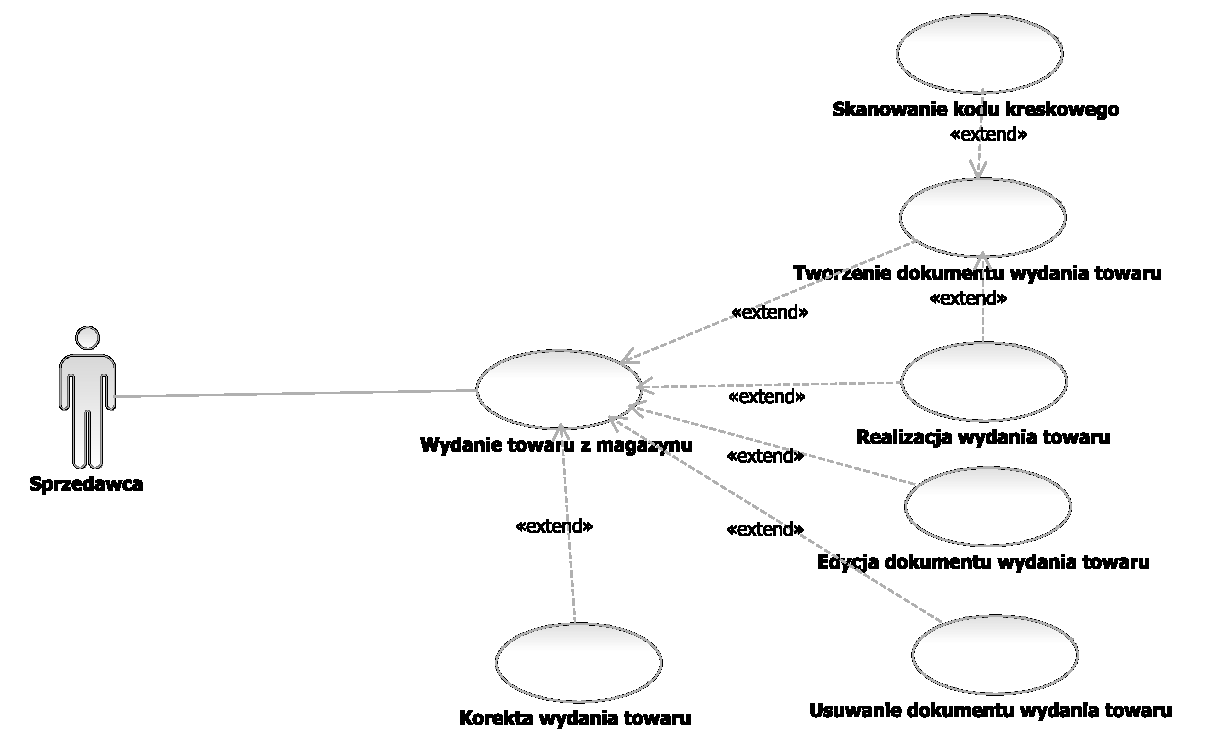
\includegraphics[scale=0.6]{../img/usecase/Sprzedaz.pdf}
  \caption{Diagram przypadków użycia dla sprzedaży.}
  \label{fig:Sprzedaz}
\end{figure}

\newpage
\singlespacing
\subsection{Wydanie towaru z magazynu}
\begin{usecase}
  \addtitle{PU12}{Wydanie towaru z magazynu}
  \addfield{Priorytet:}{wysoki}
  \addfield{Aktor główny:}{Sprzedawca}
  \addfield{Warunki początkowe:}{Aktor został uwierzytelniony.}
  % Warunki końcowe (brak).
  \addscenario{Scenariusz główny:}{
  \item Aktor wybiera opcję wydania towaru z magazynu.
  \item System wyświetla listę dokumentów WZ wraz z opcjami do zarządzania dokumentami wydania towaru.
  }
  \addfield{Wymagania funkcjonalne:}{5.}
\end{usecase}

\begin{figure}[H]
  \centering
  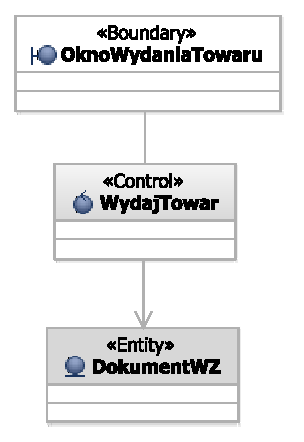
\includegraphics[angle=\ecbangle, scale=\ecbscale]{../img/usecase/pu12ecb.pdf}
  \caption{\ecbcaption12}
\end{figure}
\newpage
\begin{figure}[H]
  \centering
  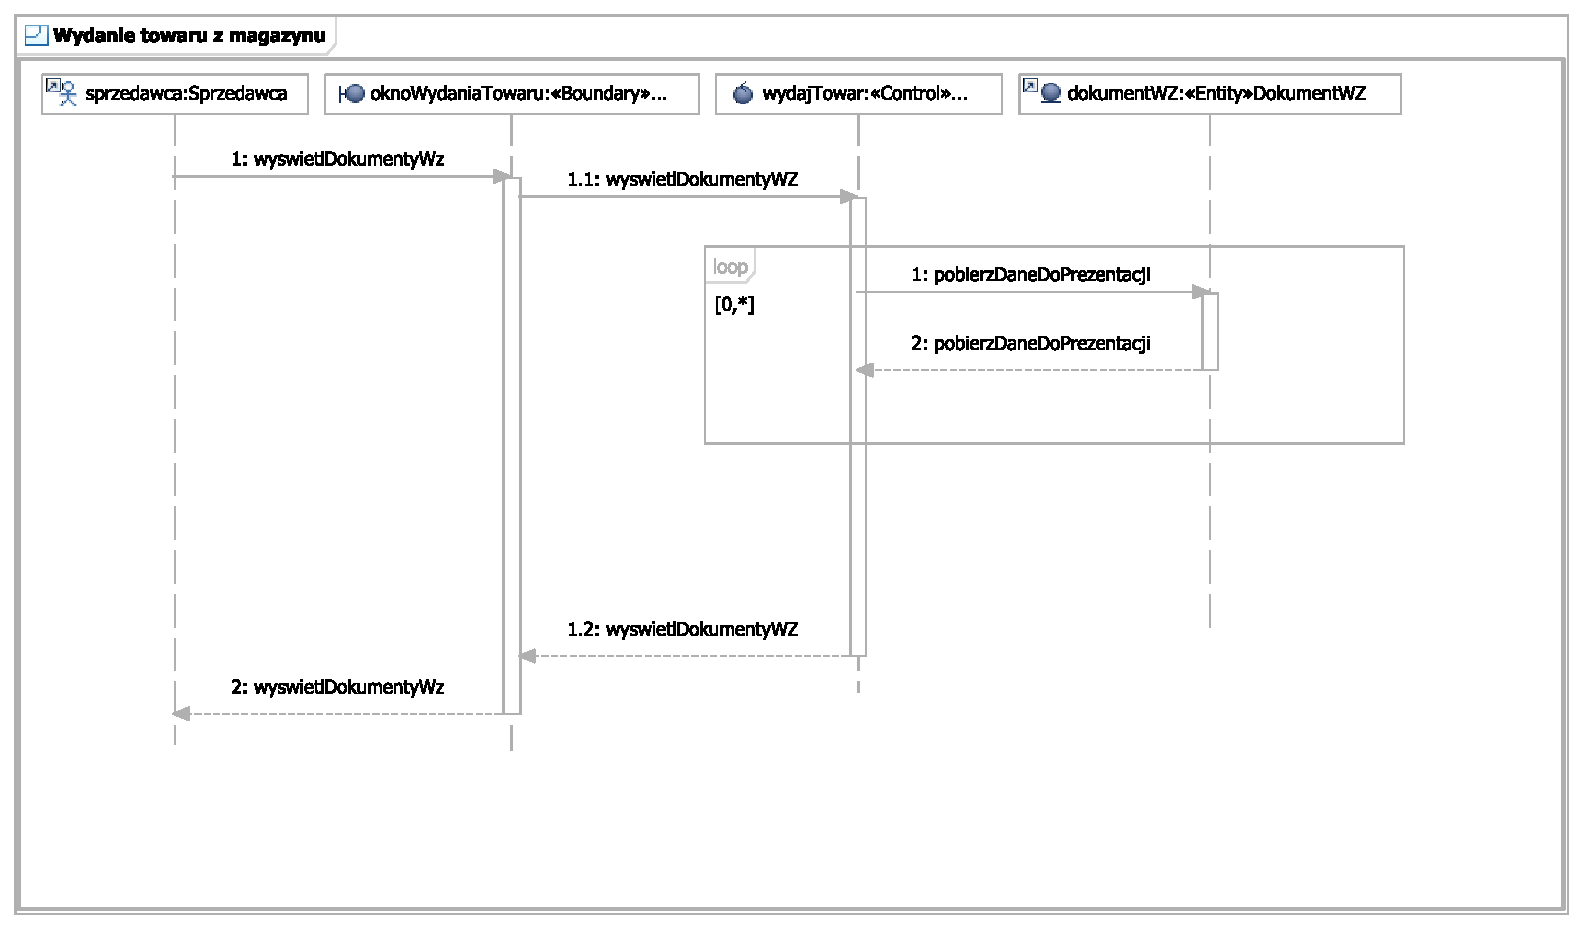
\includegraphics[angle=\seqangle, scale=\seqscale]{../img/usecase/pu12seq.pdf}
  \caption{\seqcaption12}
\end{figure}
\newpage

\subsection{Tworzenie dokumentu wydania towaru}
\begin{usecase}
  \addtitle{PU13}{Tworzenie dokumentu wydania towaru}
  \addfield{Priorytet:}{wysoki}
  \addfield{Aktor główny:}{Sprzedawca}
  \addfield{Rozszerza przypadki:}{PU12}
  \addfield{Warunki początkowe:}{Aktor został uwierzytelniony.}
  \additemizedfield{Warunki końcowe:}{ 
    \item Dokument wydania towaru został zapisany w systemie.
    \item Aktor otrzymuje informacje o poprawnym dodaniu dokumentu do systemu.
    \item Użytkownik może wyświetlić dokument na liście dokumentów wydania towaru. 
    \item Ilość przechowywanego towaru została zaktualizowana o ilość towaru zapisanego w dokumencie wydania towaru.
    \item Ilość przechowywanego towaru jest zgodna z warunkami poprawności danych przedstawionymi w \ref{dziedzina-problemu}.
  }
  \addscenario{Scenariusz główny:}{
    \item Aktor wybiera opcję utworzenia nowego dokumentu wydania towaru.
    \item System wyświetla formularz nowego dokumentu wydania towaru.
    \item Aktor wypełnia podstawowe dane dokumentu.
    \item Aktor wybiera kontrahenta operacji.
    \item Aktor wybiera towary, które będą wydane kontrahentowi.
    \item Aktor wskazuje ilość oraz cenę jednostkową wydawanego towaru.
    \item Aktor wybiera opcję zapisania dokumentu.
    \item System informuje aktora, że dane zostały poprawnie zaktualizowane.
  }
  \addscenario{Scenariusz alternatywny:} {
    \item [3.a] Aktor nie podał wymaganych pól formularza:
      \begin{enumerate}
        \item[1--4.] Jak w scenariuszu głównym.
        \item[5.] System wyświetla powiadomienie o konieczności podania wymaganych informacji.
        \item[6.] Aktor wraca do punktu 3.  
      \end{enumerate}
    \item [3.b] Aktor podał błędne wartości pól formularza:
      \begin{enumerate}
        \item[1--4.] Jak w scenariuszu głównym.
        \item[5.] System wyświetla powiadomienie o błędnych polach formularza.
        \item[6.] Aktor wraca do punktu 3.
      \end{enumerate}
     \item[5.a] Aktor wybrał ten sam towar co najmniej dwa razy.
       \begin{enumerate}
       \item[1--5.] Jak w scenariuszu głównym.
       \item[6.] System informuje aktora, że co najmniej dwa razy wybrał ten sam towar, podane ilości towaru zostaną więc zsumowane.
       \item[7.] System wyświetla zsumowane wartości dla tych samych towarów.
       \item[8--...] Jak w scenariuszu głównym.
       \end{enumerate}
  }
  \addfield{Zakres przetwarzanych danych:} {
    Pola dokumentu wydania towaru takie jak przedstawione w rozdziale \ref{dziedzina-problemu}.
  }
  \addfield{Warunki poprawności danych:}{
    Warunki poprawności takie jak przedstawione w rozdziale \ref{dziedzina-problemu}.
  }
  \addfield{Wymagania funkcjonalne:}{5.1}
\end{usecase}

\begin{figure}[H]
  \centering
  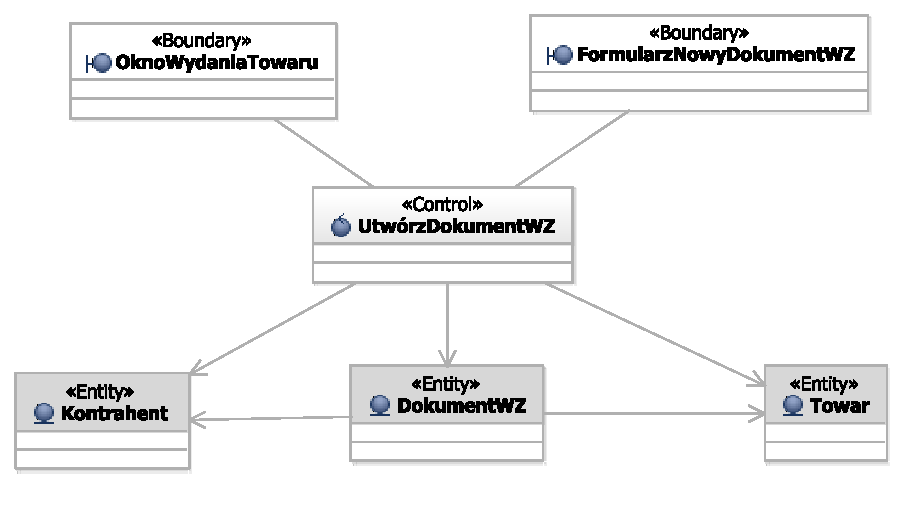
\includegraphics[angle=\ecbangle, scale=\ecbscale]{../img/usecase/pu13ecb.pdf}
  \caption{\ecbcaption13}
\end{figure}
\newpage
\begin{figure}[H]
  \centering
  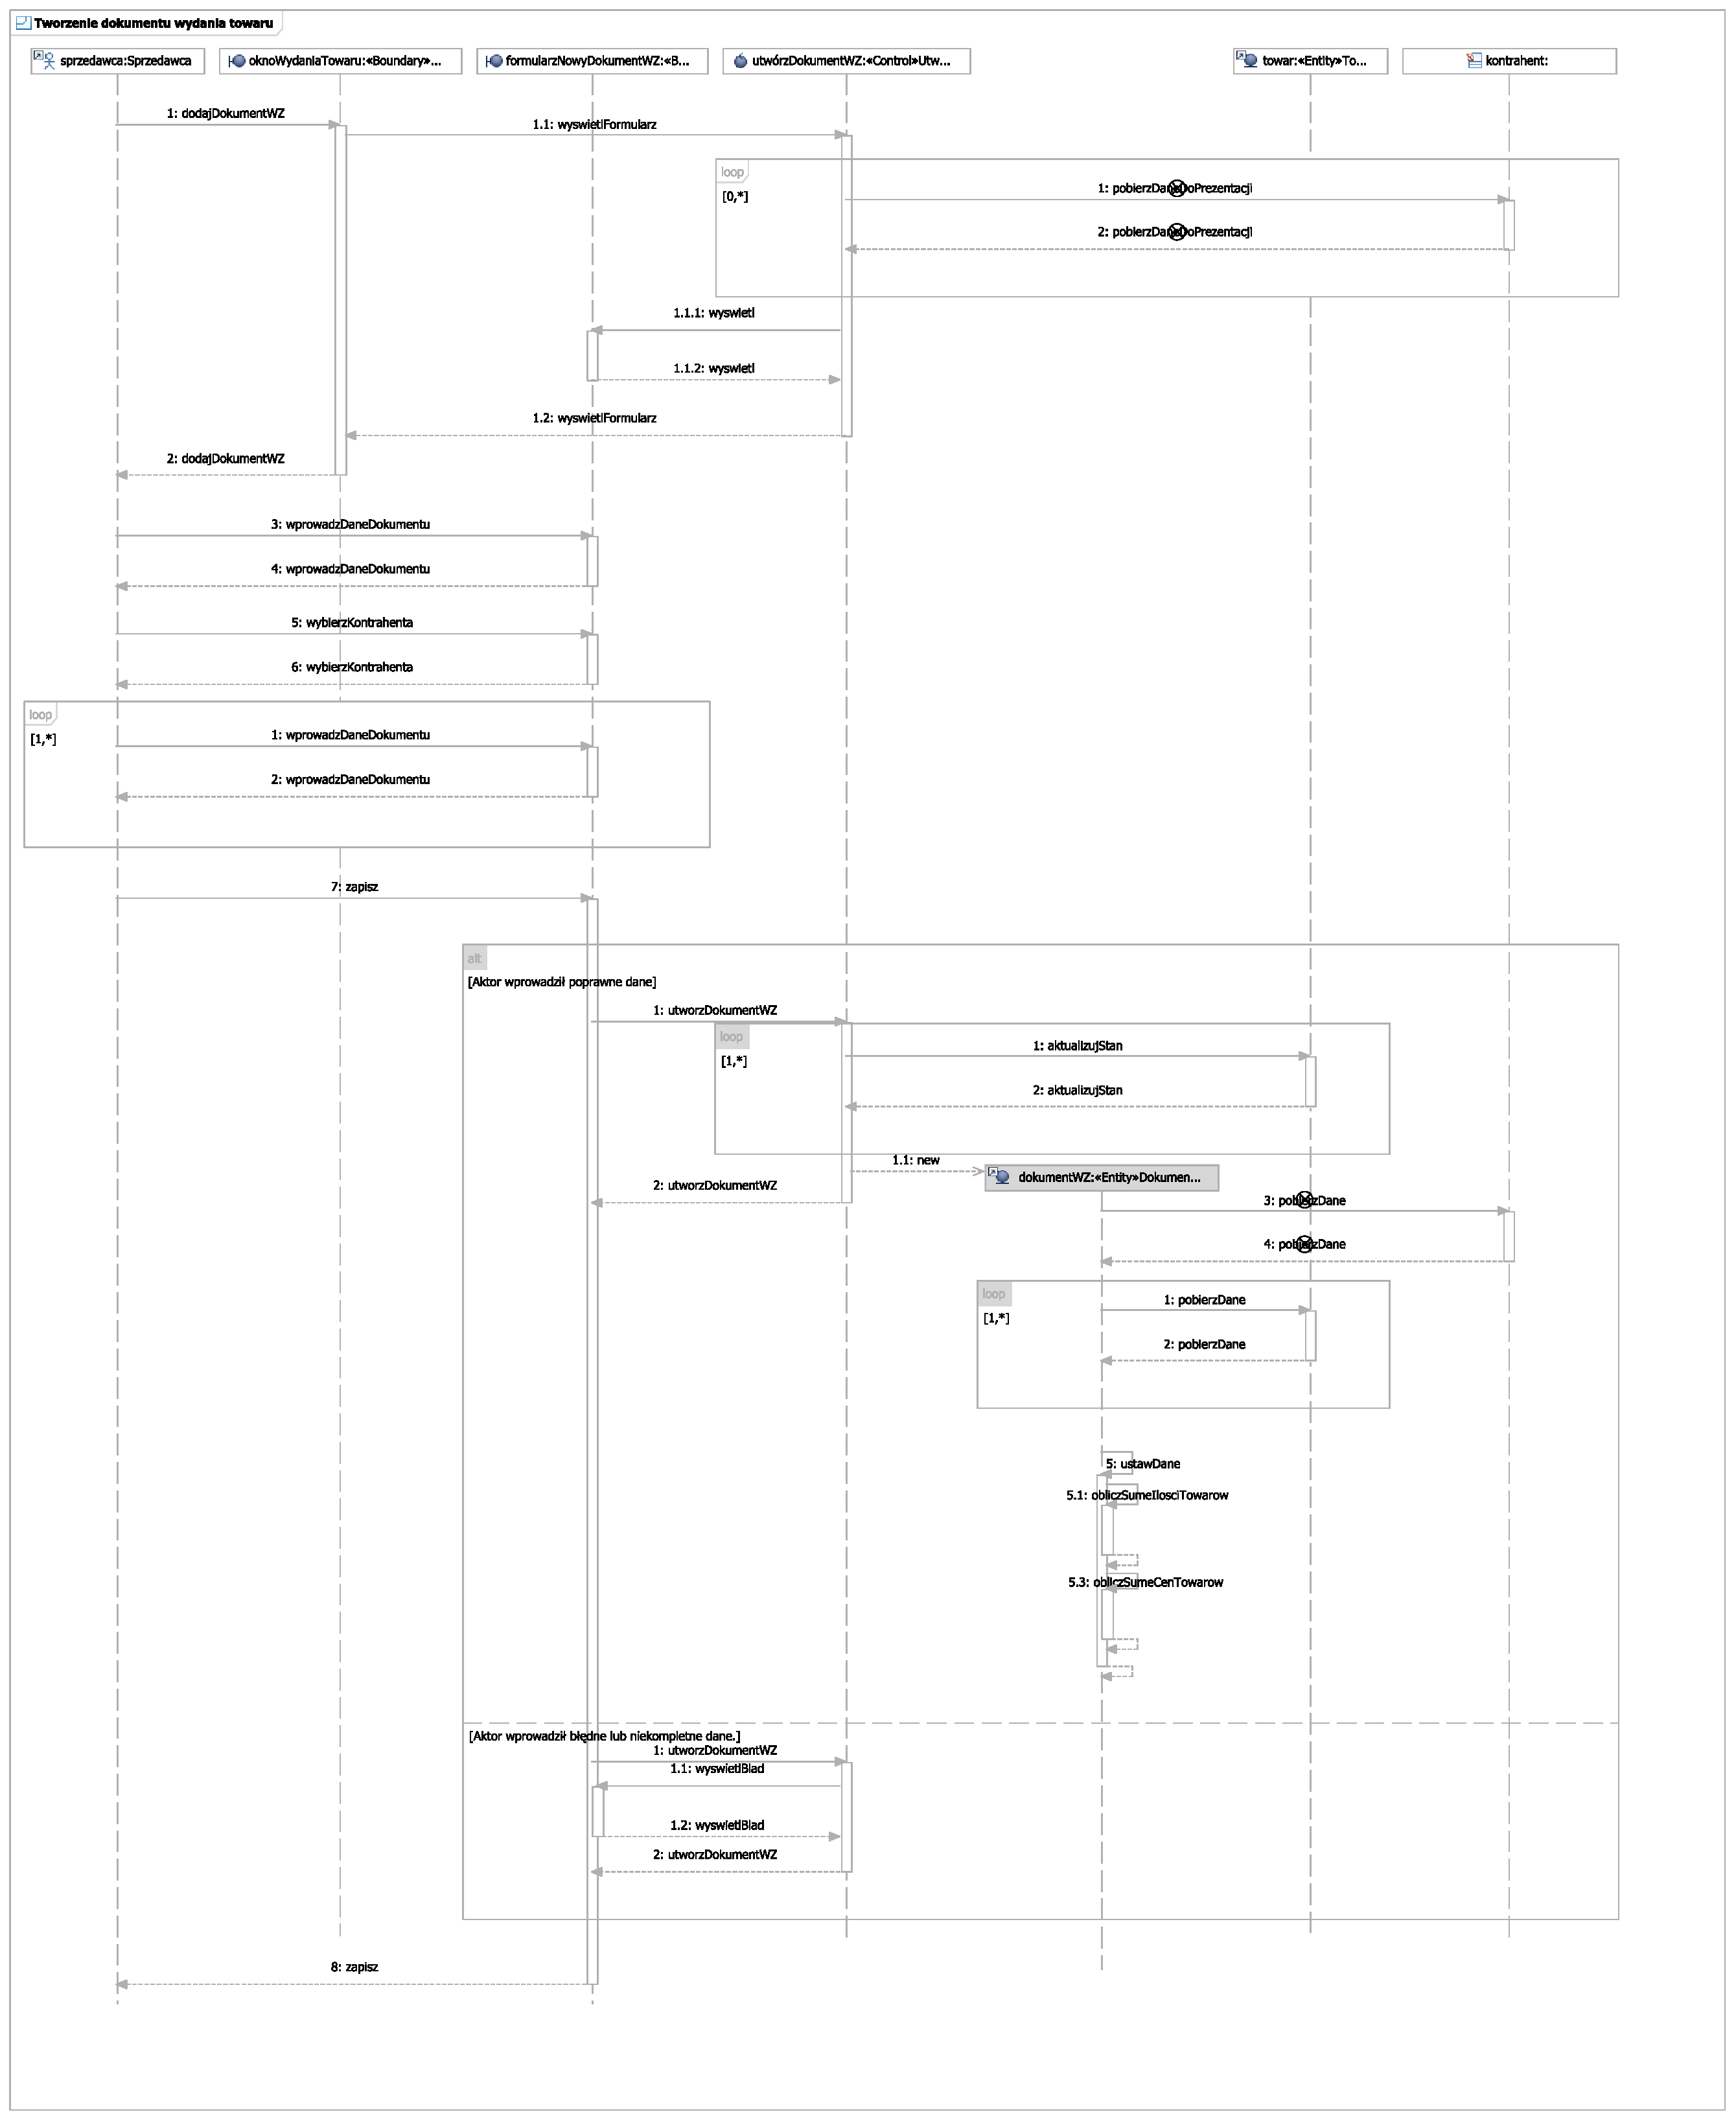
\includegraphics[angle=\seqangle, scale=0.35]{../img/usecase/pu13seq.pdf}
  \caption{\seqcaption13}
\end{figure}
\newpage

\subsection{Edycja dokumentu wydania towaru}
\begin{usecase}
  \addtitle{PU14}{Edycja dokumentu wydania towaru}
  \addfield{Priorytet:}{wysoki}
  \addfield{Aktor główny:}{Sprzedawca}
  \addfield{Rozszerza przypadki:}{PU12}
  \additemizedfield{Warunki początkowe:}{
    \item Aktor został uwierzytelniony.
    \item Operacja wydania towaru, którego dotyczy wybrany dokument, nie została jeszcze zrealizowana.
  }
  \additemizedfield{Warunki końcowe:}{ 
    \item Dane dokumentu zostały zaktualizowane w systemie.
    \item Aktor otrzymuje informację o poprawnej aktualizacji dokumentu.
    \item Użytkownik może wyświetlić dane dokumentu na liście dokumentów wydania towaru. 
    \item Ilość przechowywanego towaru została zaktualizowana o ilość towaru zapisanego w dokumencie wydania towaru.
    \item Ilość przechowywanego towaru jest zgodna z warunkami poprawności danych przedstawionymi w \ref{dziedzina-problemu}.
  }
  \addscenario{Scenariusz główny:}{
    \item Aktor wybiera opcję edycji wybranego dokumentu wydania towaru.
    \item System wyświetla formularz edycji dokumentu wydania towaru.
    \item Aktor wypełnia podstawowe dane dokumentu (oprócz pól wykluczonych z edycji).
    \item Aktor aktualizuje listę towarów, ich ilości oraz ceny jednostkowe.
    \item Aktor wybiera opcję aktualizacji dokumentu.
    \item System informuje aktora, że dane zostały poprawnie zaktualizowane.
  }
  \addscenario{Scenariusz alternatywny:} {
    \item [3.a] Aktor nie podał wymaganych pól formularza:
      \begin{enumerate}
        \item[1--4.] Jak w scenariuszu głównym.
        \item[5.] System wyświetla powiadomienie o konieczności podania wymaganych informacji.
        \item[6.] Aktor wraca do punktu 3.  
      \end{enumerate}
    \item [3.b] Aktor podał błędne wartości pól formularza:
      \begin{enumerate}
        \item[1--4.] Jak w scenariuszu głównym.
        \item[5.] System wyświetla powiadomienie o błędnych polach formularza.
        \item[6.] Aktor wraca do punktu 3.
      \end{enumerate}
     \item[4.a] Aktor wybrał ten sam towar co najmniej dwa razy.
       \begin{enumerate}
       \item[1--4.] Jak w scenariuszu głównym.
       \item[5.] System informuje aktora, że co najmniej dwa razy wybrał ten sam towar, podane ilości towaru zostaną więc zsumowane.
       \item[6.] System wyświetla zsumowane wartości dla tych samych towarów.
       \item[7--...] Jak w scenariuszu głównym.
       \end{enumerate}
  }
  \addfield{Zakres przetwarzanych danych:} {
    Pola dokumentu wydania towaru takie jak przedstawione w rozdziale \ref{dziedzina-problemu}.
  }
  \addfield{Warunki poprawności danych:}{
    Warunki poprawności takie jak przedstawione w rozdziale \ref{dziedzina-problemu}.
  }
  \addfield{Wymagania funkcjonalne:}{5.2}
\end{usecase}

\begin{figure}[H]
  \centering
  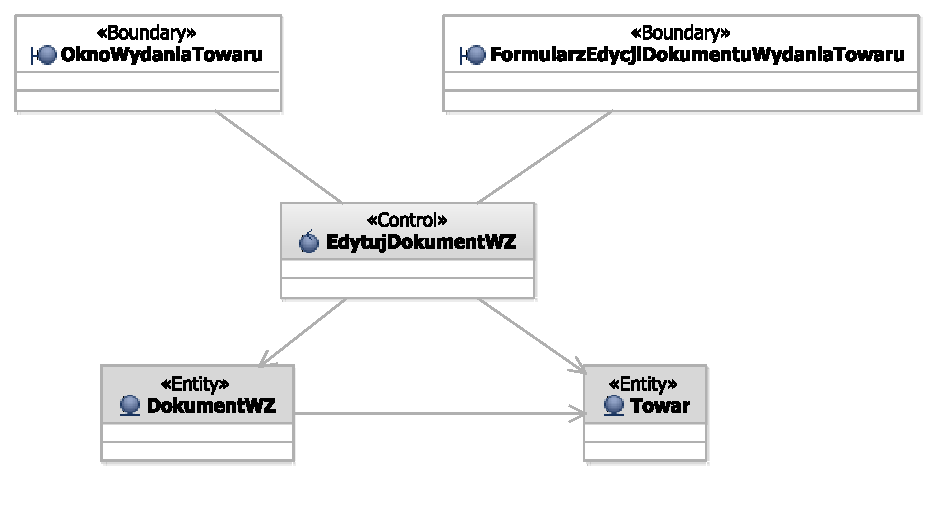
\includegraphics[angle=\ecbangle, scale=\ecbscale]{../img/usecase/pu14ecb.pdf}
  \caption{\ecbcaption14}
\end{figure}
\newpage
\begin{figure}[H]
  \centering
  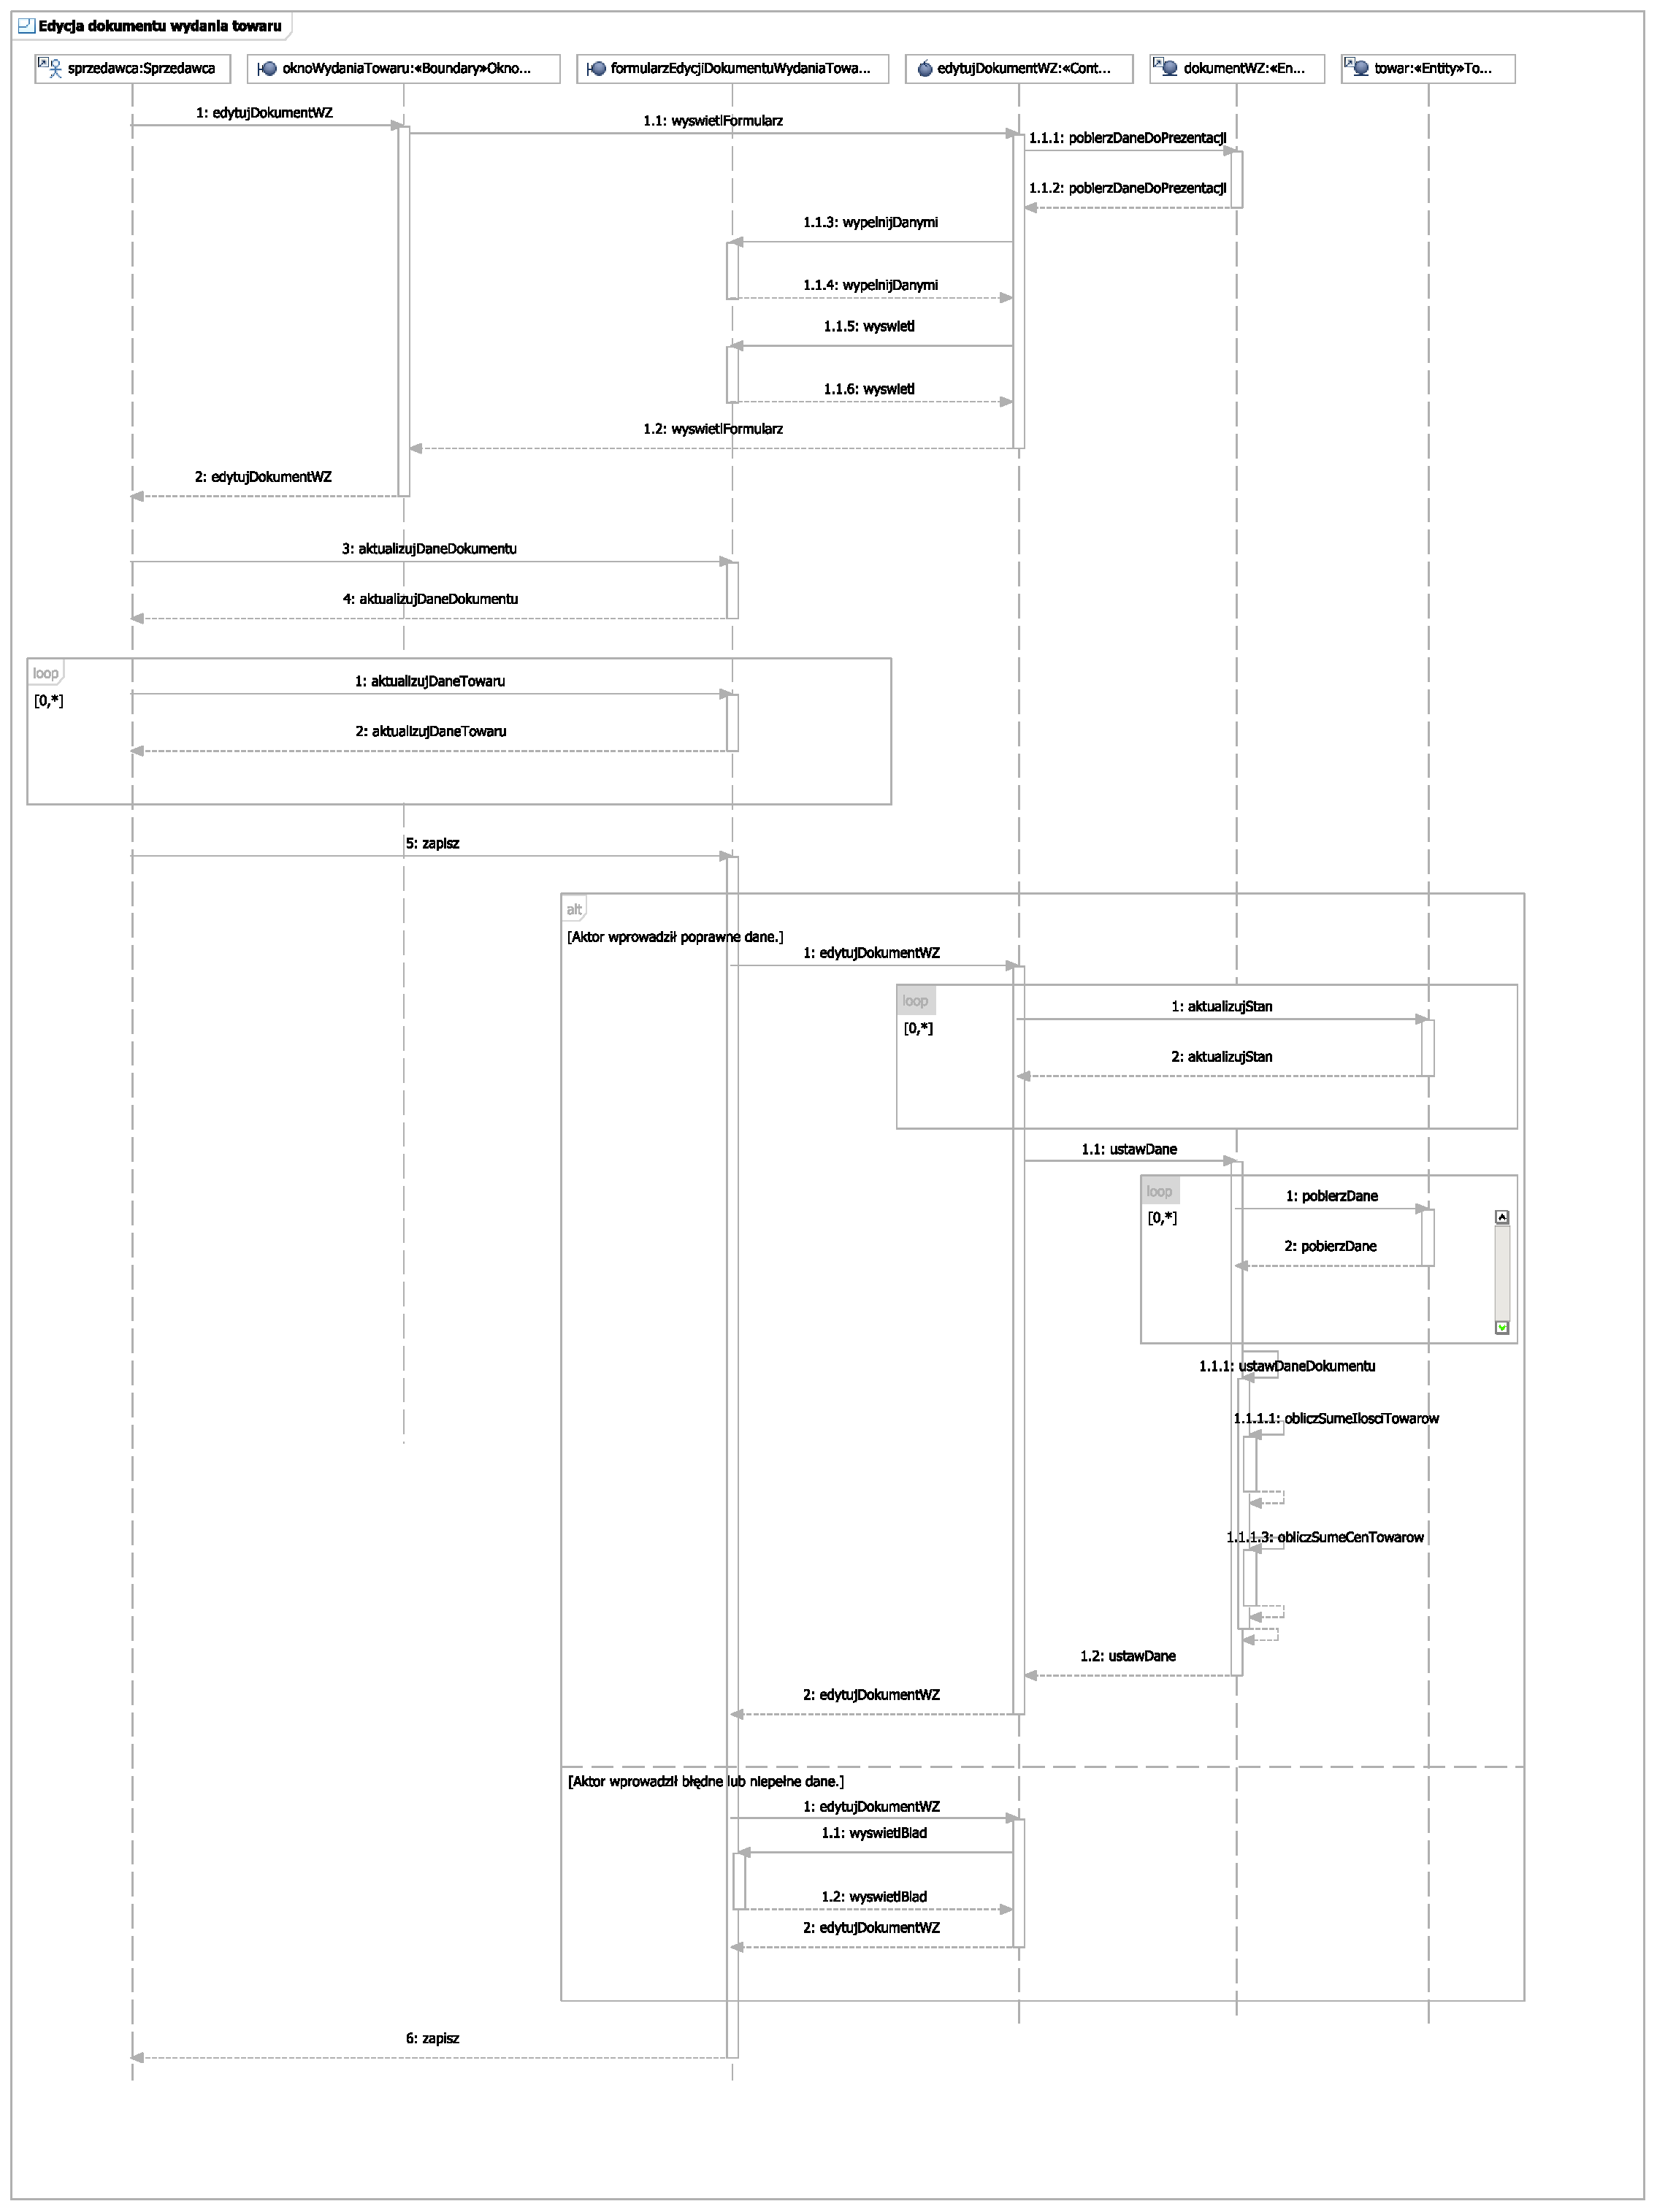
\includegraphics[angle=\seqangle, scale=\seqscalemin]{../img/usecase/pu14seq.pdf}
  \caption{\seqcaption14}
\end{figure}
\newpage

\subsection{Usuwanie dokumentu wydania towaru}
\begin{usecase}
  \addtitle{PU15}{Usuwanie dokumentu wydania towaru}
  \addfield{Priorytet:}{wysoki}
  \addfield{Aktor główny:}{Sprzedawca}
  \addfield{Rozszerza przypadki:}{PU12}
  \addfield{Warunki początkowe:}{Aktor został uwierzytelniony.}
  \additemizedfield{Warunki końcowe:}{
    \item Dane dokumentu zostały usunięte z systemu.
    \item Usunięty dokument nie jest wyświetlany na liście dokumentów wydania towaru.
    \item Stan towarów z usuniętego dokumentu jest zaktualizowany o ilości zapisane w usuwanym dokumencie.
  }
  \addscenario{Scenariusz główny:}{
    \item Aktor wybiera opcję usunięcia dokumentu wydania towaru z systemu.
    \item System prosi o potwierdzenie operacji.
    \item Aktor potwierdza usunięcie dokumentu z systemu.
    \item System wyświetla informację o pomyślnym usunięciu dokumentu z systemu.
  }
  \addscenario{Scenariusz alternatywny:}{
    \item[2.a] Aktor anuluje usunięcie dokumentu z systemu.
      \begin{enumerate}
        \item[1.--2.] Jak w scenariuszu głównym.
        \item[3.] Aktor anuluje usunięcie dokumentu z systemu.
        \item[4.] System wyświetla informację, że operacja została anulowana.
      \end{enumerate}
  }
  \addfield{Wymagania funkcjonalne:}{5.3}
\end{usecase}

\begin{figure}[H]
  \centering
  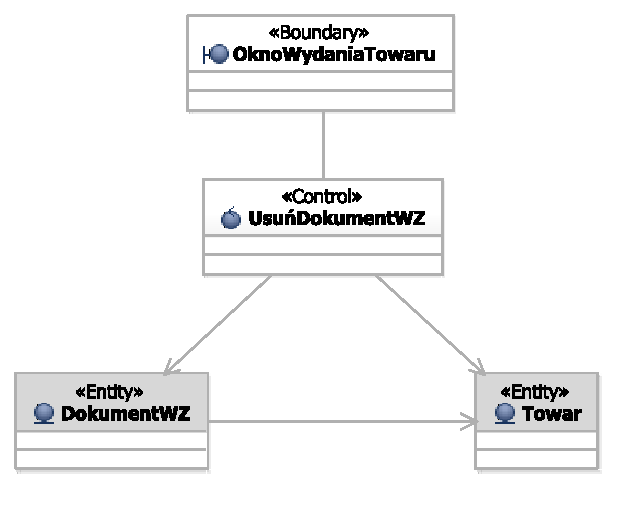
\includegraphics[angle=\ecbangle, scale=\ecbscale]{../img/usecase/pu15ecb.pdf}
  \caption{\ecbcaption15}
\end{figure}

\begin{figure}[H]
  \centering
  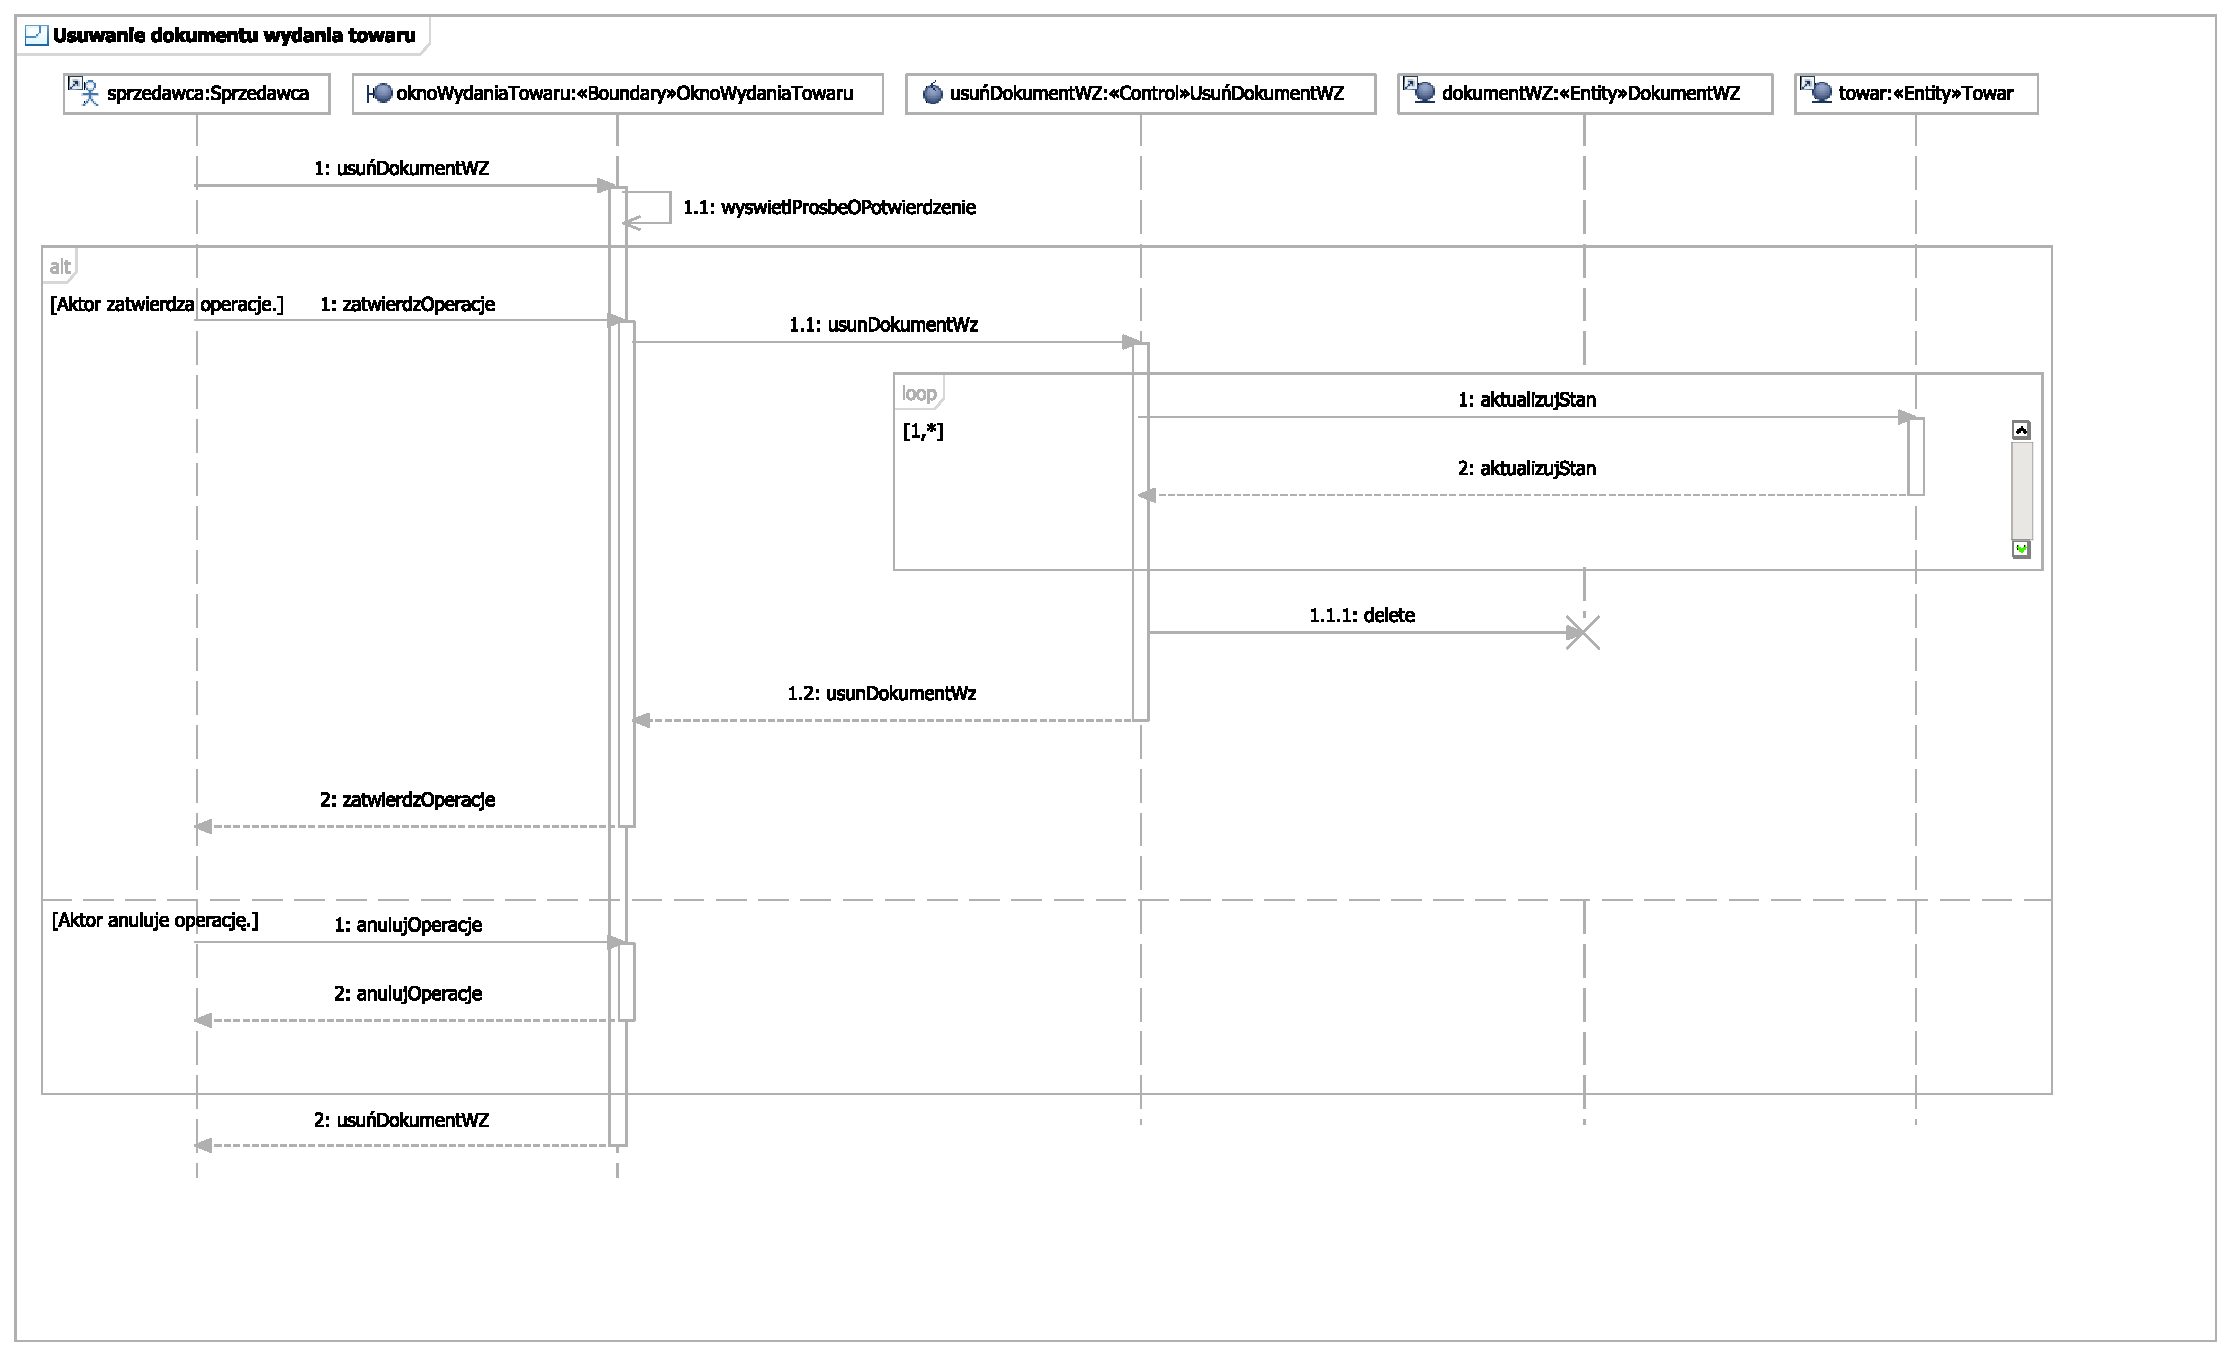
\includegraphics[angle=\seqangle, scale=0.42]{../img/usecase/pu15seq.pdf}
  \caption{\seqcaption15}
\end{figure}
\newpage

\subsection{Realizacja wydania towaru z magazynu}
\begin{usecase}
  \addtitle{PU16}{Realizacja wydania towaru z magazynu}
  \addfield{Priorytet:}{wysoki}
  \addfield{Aktor główny:}{Sprzedawca}
  \addfield{Rozszerza przypadki:}{PU12}
  \additemizedfield{Warunki początkowe:}{
    \item Aktor został uwierzytelniony.
    \item Wybrane wydanie towaru nie zostało jeszcze zrealizowane.}
  \additemizedfield{Warunki końcowe:} {
    \item Dokument wydania towaru został oznaczony jako zrealizowany.
    \item Możliwe jest utworzenie korekty do zrealizowanego dokumentu wydania towaru.
  }
  \addscenario{Scenariusz główny:}{
     \item Aktor wybiera opcję wydania towaru z magazynu.
     \item System prosi o potwierdzenie realizacji wydania towaru z magazynu.
     \item Aktor potwierdza realizację wydania towaru z magazynu.
     \item System oznacza dokument wydania towaru jako zrealizowany.
  }
 \addscenario{Scenariusz alternatywny:}{
    \item[4.a] Aktor anuluje realizację wydania towaru.
      \begin{enumerate}
        \item[1.--2.] Jak w scenariuszu głównym.
        \item[3.] Aktor anuluje realizację dokumentu.
        \item[4.] System wyświetla informację, że operacja została anulowana.
      \end{enumerate}
  }
  \addfield{Wymagania funkcjonalne:}{5.4}
\end{usecase}

\begin{figure}[H]
  \centering
  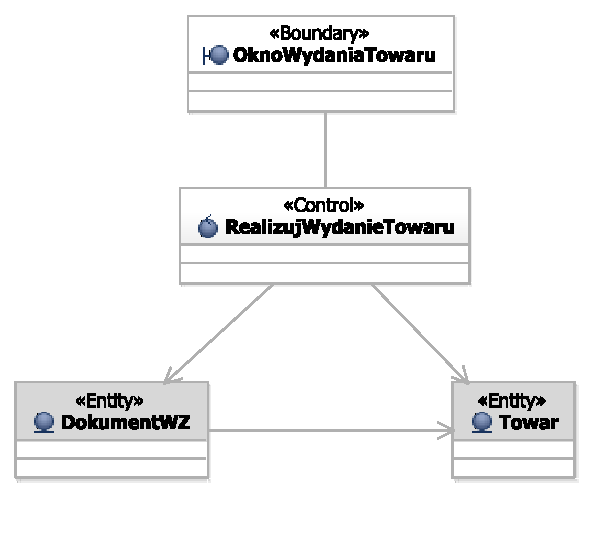
\includegraphics[angle=\ecbangle, scale=\ecbscale]{../img/usecase/pu16ecb.pdf}
  \caption{\ecbcaption16}
\end{figure}

\begin{figure}[H]
  \centering
  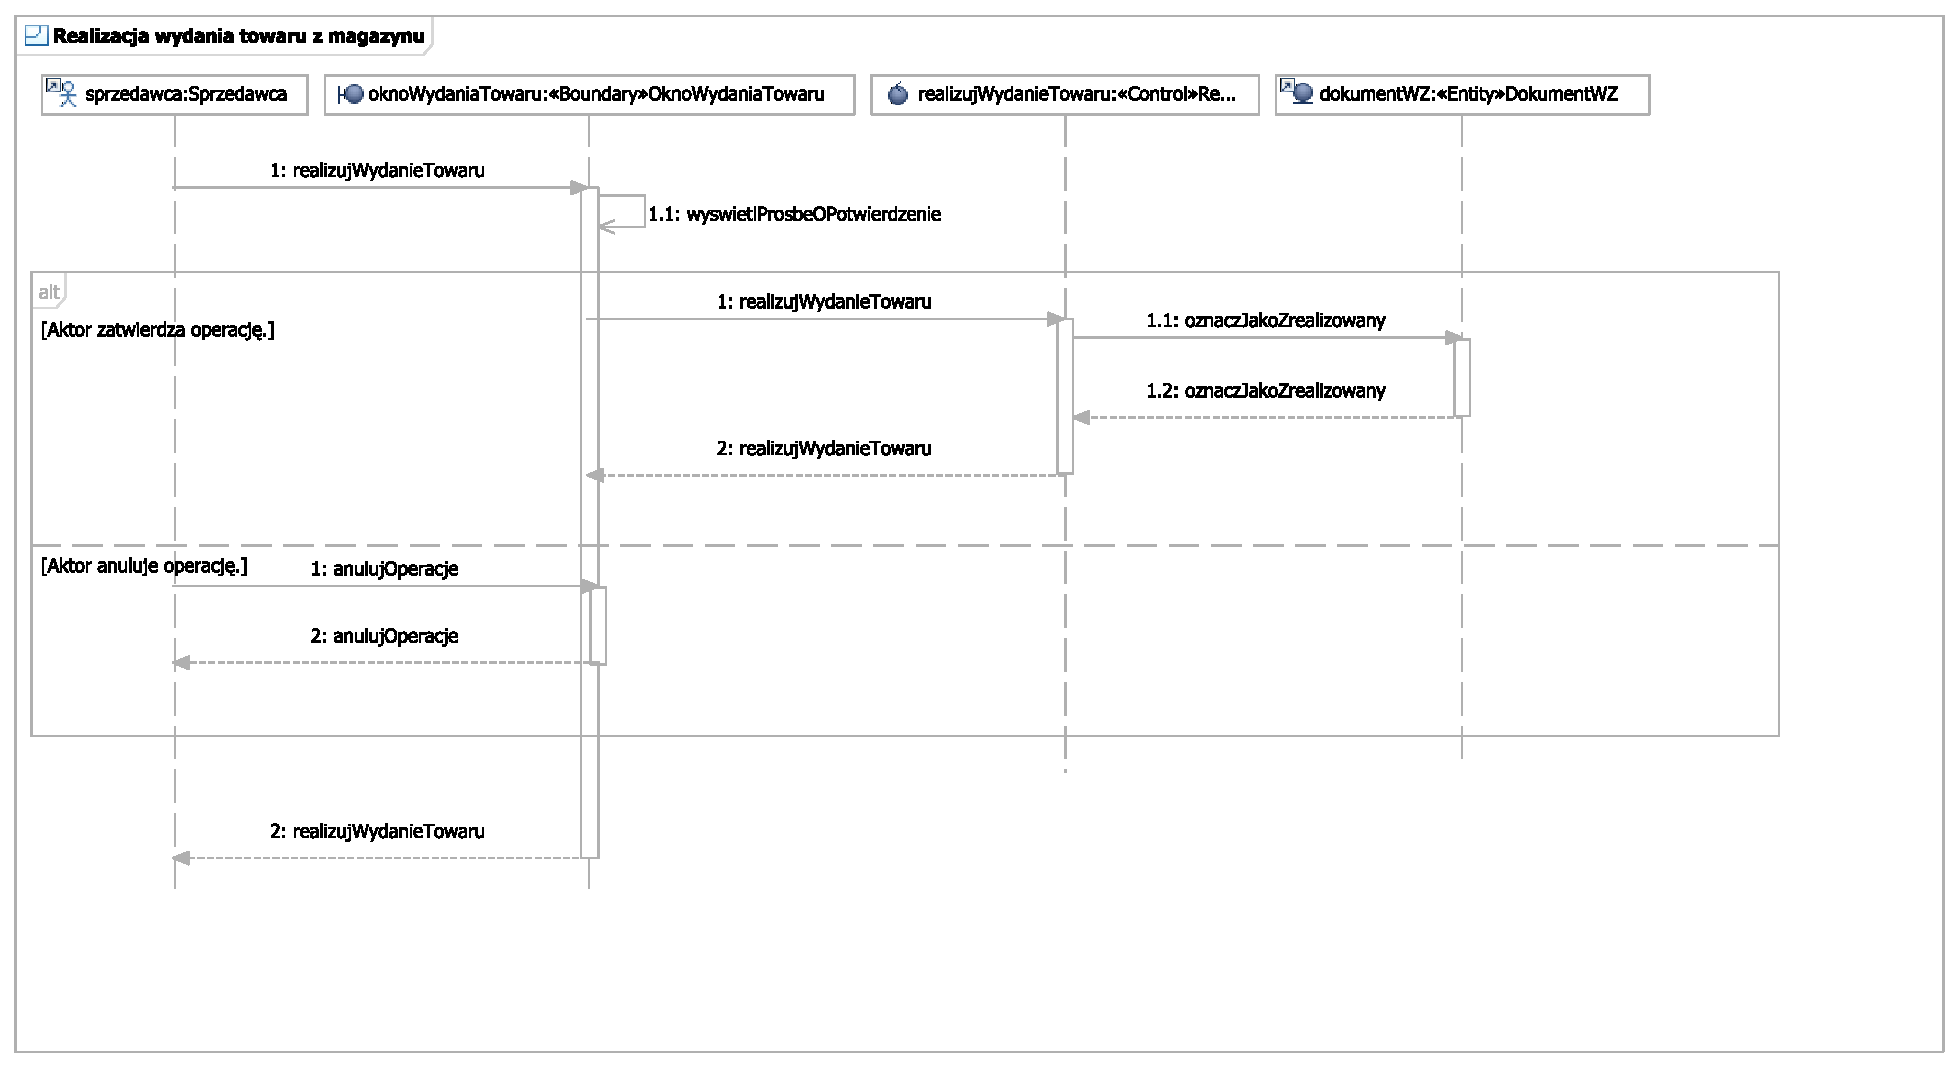
\includegraphics[angle=\seqangle, scale=0.5]{../img/usecase/pu16seq.pdf}
  \caption{\seqcaption16}
\end{figure}
\newpage

\subsection{Korekta wydania towaru}
\begin{usecase}
  \addtitle{PU17}{Korekta wydania towaru}
  \addfield{Priorytet:}{wysoki}
  \addfield{Aktor główny:}{Sprzedawca}
  \addfield{Rozszerza przypadki:}{PU12, PU13}
  \additemizedfield{Warunki początkowe:}{
     \item Aktor został uwierzytelniony.
     \item Wybrany dokument wydania towaru został już zrealizowany.
  }
  \additemizedfield{Warunki końcowe:}{ 
    \item Dokument korekty wydania towaru został zapisany w systemie.
    \item Ilość przechowywanych towarów została zaktualizowana zgodnie z wartością podaną na korekcie. 
    \item Ilość przechowywanego towaru jest zgodna z warunkami poprawności danych przedstawionymi w \ref{dziedzina-problemu}.
  }
  \addscenario{Scenariusz główny:}{
    \item Aktor wybiera opcję utworzenia korekty dla wskazanego dokumentu przyjęcia towaru.
    \item System wyświetla formularz nowej korekty. 
    \item Aktor wypełnia podstawowe dane korekty.
    \item Aktor wybiera towary, które podlegają zwrotowi oraz ich cenę.
    \item Aktor wybiera opcję zapisania korekty.
    \item System informuje aktora, że dane zostały poprawnie zaktualizowane.
  }
  \addscenario{Scenariusz alternatywny:} {
    \item [3.a] Aktor nie podał wymaganych pól formularza:
      \begin{enumerate}
        \item[1--4.] Jak w scenariuszu głównym.
        \item[5.] System wyświetla powiadomienie o konieczności podania wymaganych informacji.
        \item[6.] Aktor wraca do punktu 3.  
      \end{enumerate}
    \item [3.b] Aktor podał błędne wartości pól formularza:
      \begin{enumerate}
        \item[1--4.] Jak w scenariuszu głównym.
        \item[5.] System wyświetla powiadomienie o błędnych polach formularza.
        \item[6.] Aktor wraca do punktu 3.
      \end{enumerate}
     \item[5.a] Aktor wybrał ten sam towar co najmniej dwa razy.
       \begin{enumerate}
       \item[1--5.] Jak w scenariuszu głównym.
       \item[6.] System informuje aktora, że co najmniej dwa razy wybrał ten sam towar, podane ilości towaru zostaną więc zsumowane.
       \item[7.] System wyświetla zsumowane wartości dla tych samych towarów.
       \item[8--...] Jak w scenariuszu głównym.
       \end{enumerate}
  }
  \addfield{Zakres przetwarzanych danych:} {
    Pola dokumentu wydania towaru takie jak przedstawione w rozdziale \ref{dziedzina-problemu}.
  }
  \addfield{Warunki poprawności danych:}{
    Warunki poprawności takie jak przedstawione w rozdziale \ref{dziedzina-problemu}.
  }
  \addfield{Wymagania funkcjonalne:}{5.5}
\end{usecase}

\begin{figure}[H]
  \centering
  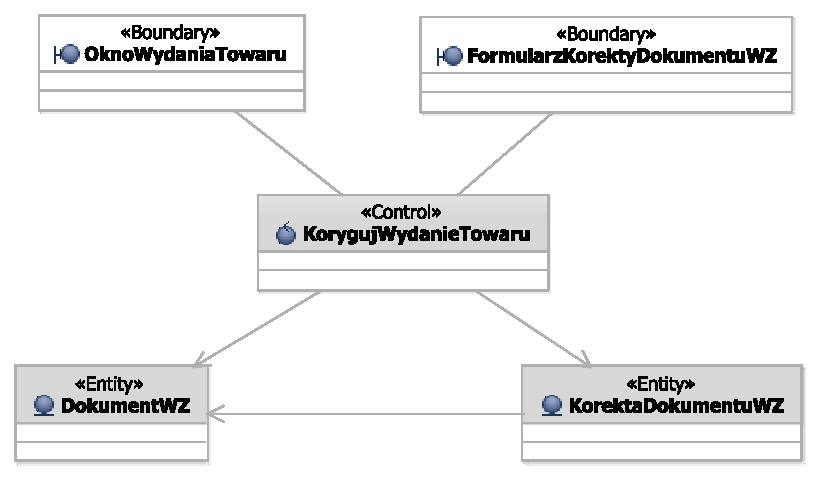
\includegraphics[angle=\ecbangle, scale=\ecbscale]{../img/usecase/pu17ecb.pdf}
  \caption{\ecbcaption17}
\end{figure}
\newpage
\begin{figure}[H]
  \centering
  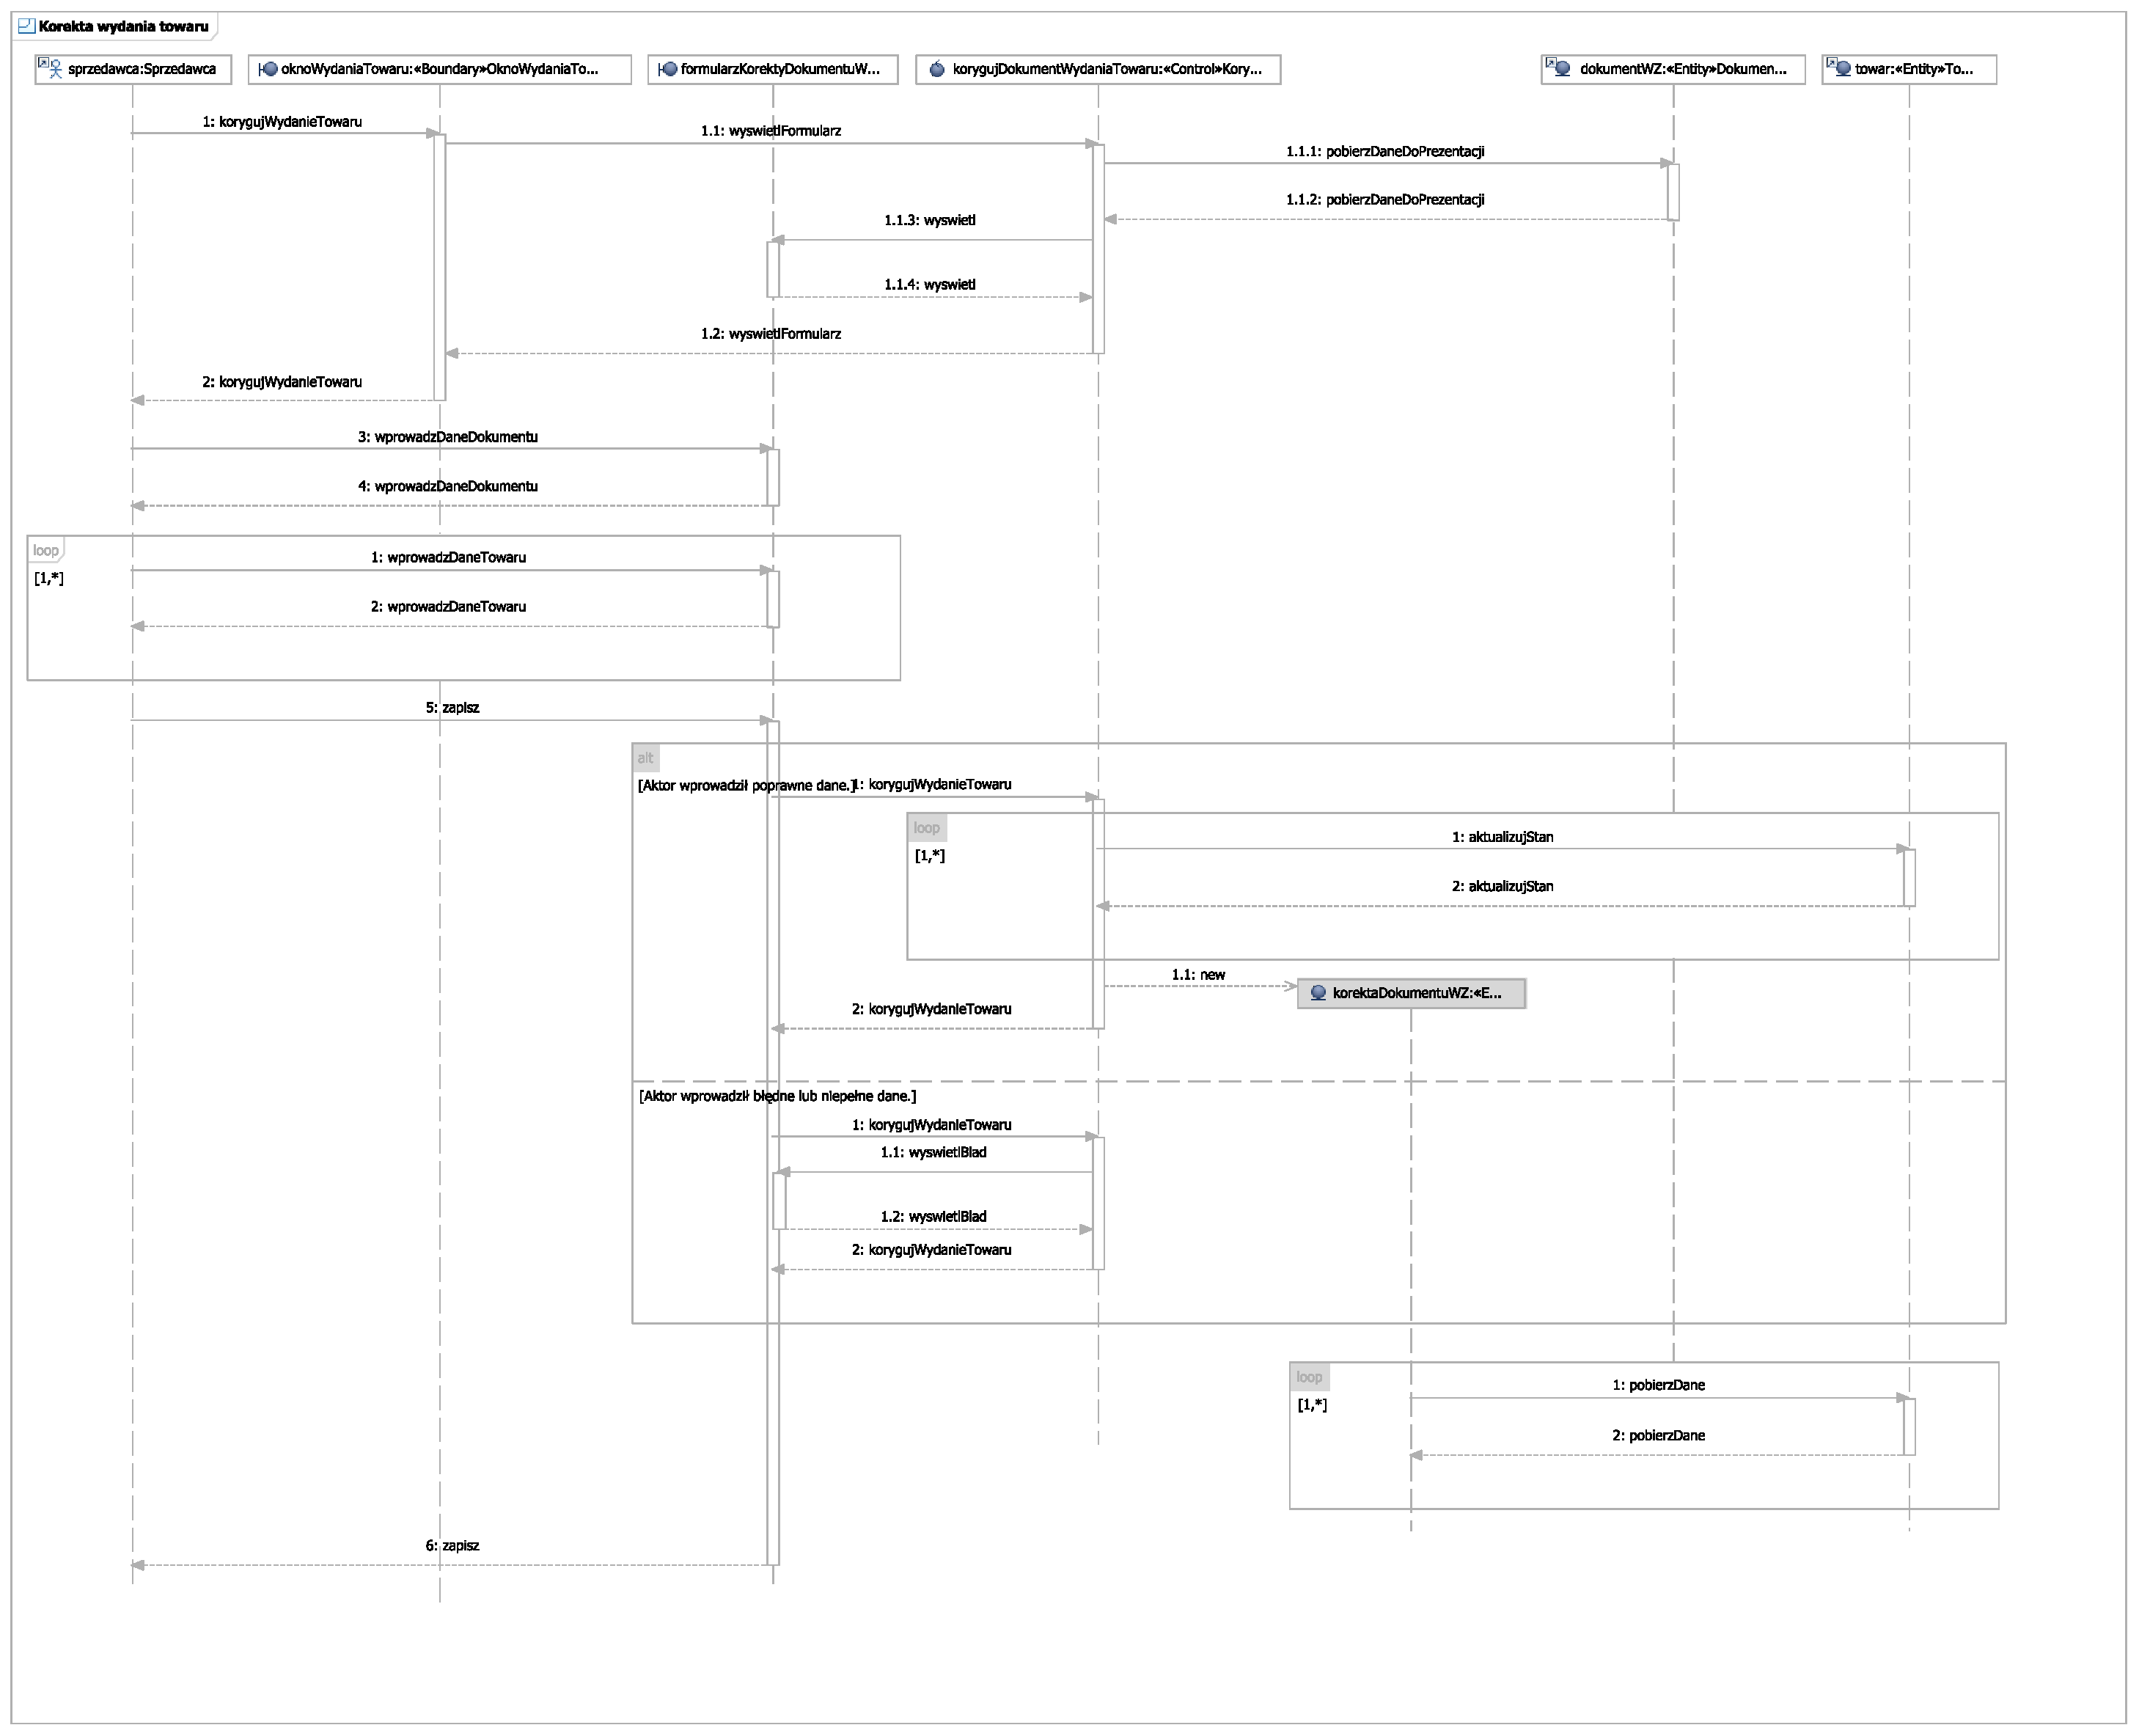
\includegraphics[angle=\seqangle, scale=0.32]{../img/usecase/pu17seq.pdf}
  \caption{\seqcaption17}
\end{figure}
\newpage






\section{Zarządzanie towarami}
Magazynier jest osobą odpowiedzialną za odwzorowanie aktualnego stanu
magazynu w systemie. Wprowadza dane towarów do systemu, a także
aktualizuje ich stan. Ponadto zarządza on dokumentacją przyjęć towaru (PZ) do
magazynu oraz danymi kontrahentów. W razie potrzeby może zwrócić
przyjęty towar oraz skorygować aktualny stan towaru 
(np. gdy towar straci swój termin ważności). Diagram przedstawiający opisane przypadki użycia
został zaprezentowany na rysunku \ref{fig:ZarzadzanieTowarami}.

\begin{figure}[H]
  \centering
  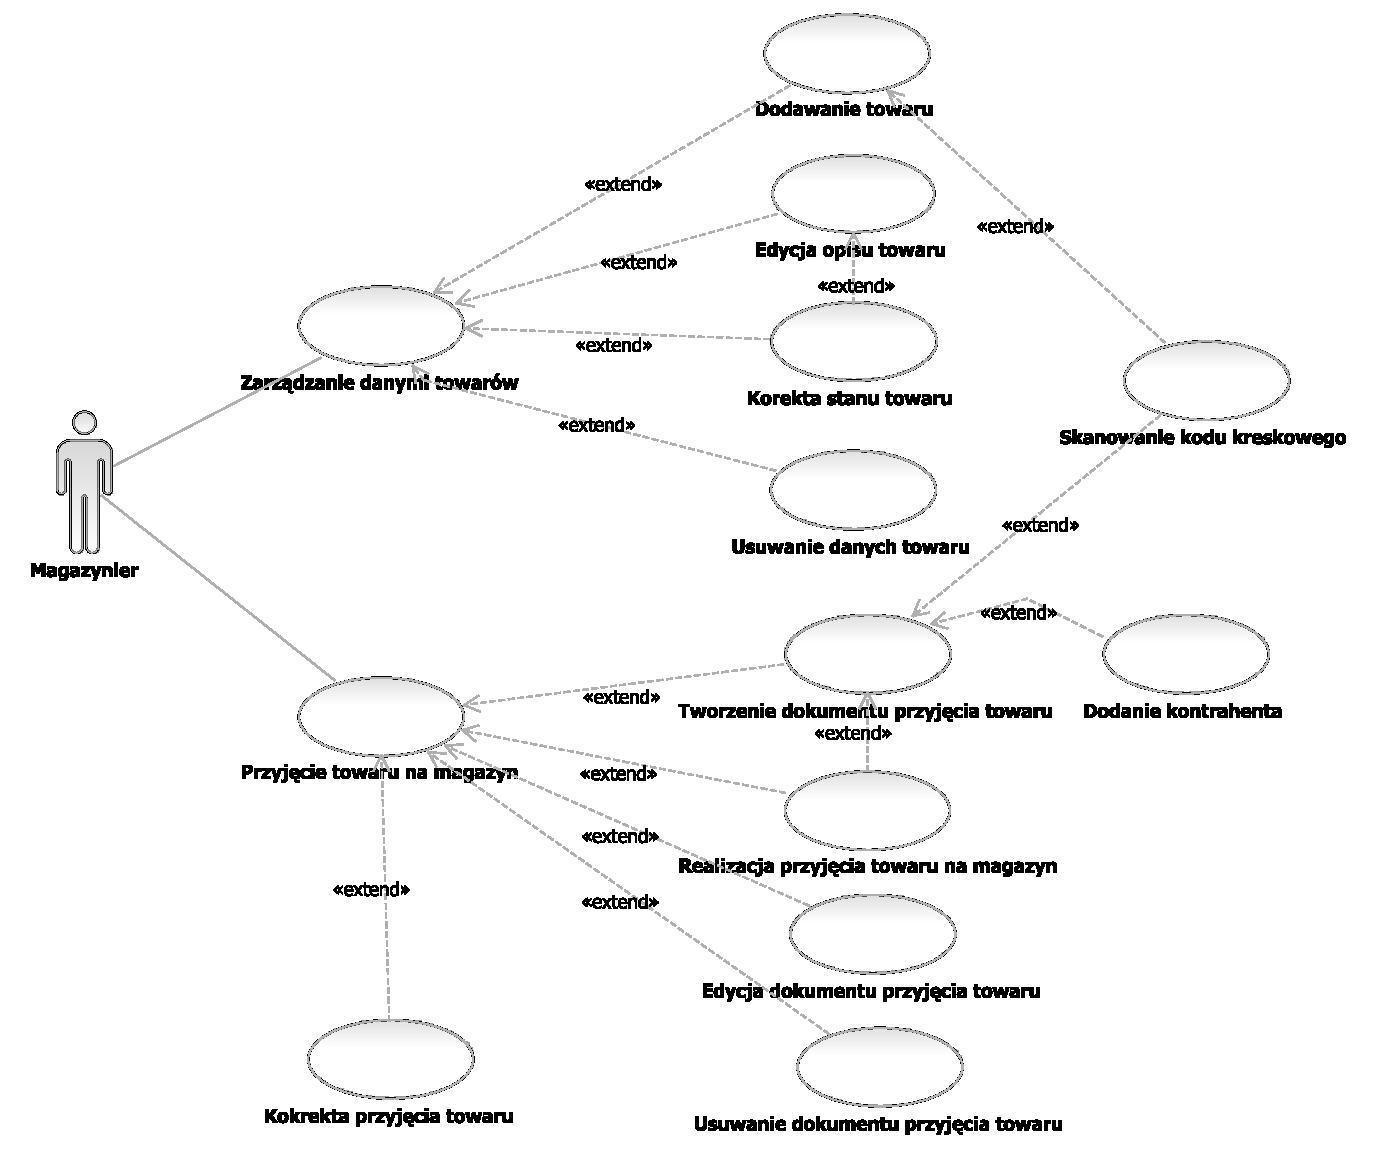
\includegraphics[scale=0.6]{../img/usecase/ZarzadzanieTowarami.pdf}
  \caption{Diagram przypadków użycia dla zarządzania towarami.}
  \label{fig:ZarzadzanieTowarami}
\end{figure}

\newpage
\singlespacing
\subsection{Zarządzanie danymi towarów}

\begin{usecase}
  \addtitle{PU18}{Zarządzanie danymi towarów}
  \addfield{Priorytet:}{wysoki}
  \addfield{Aktor główny:}{Magazynier}
  \addfield{Warunki początkowe:}{Aktor został uwierzytelniony.}
  % Warunki końcowe (brak).
  \addscenario{Scenariusz główny:}{
  \item Aktor wybiera opcję przeglądania listy towarów w magazynie.
  \item System wyświetla listę towarów w magazynie wraz z opcjami zarządzania danymi dokumentów.
  }
  \addfield{Wymagania funkcjonalne:}{2.}
\end{usecase}

\begin{figure}[H]
  \centering
  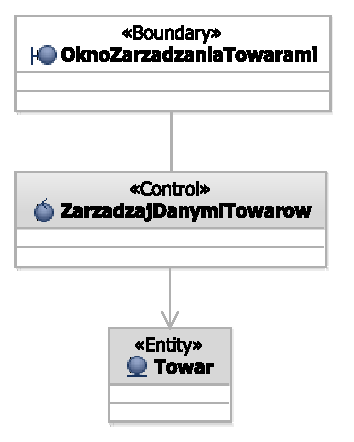
\includegraphics[angle=\ecbangle, scale=\ecbscale]{../img/usecase/pu18ecb.pdf}
  \caption{\ecbcaption18}
\end{figure}
\newpage
\begin{figure}[H]
  \centering
  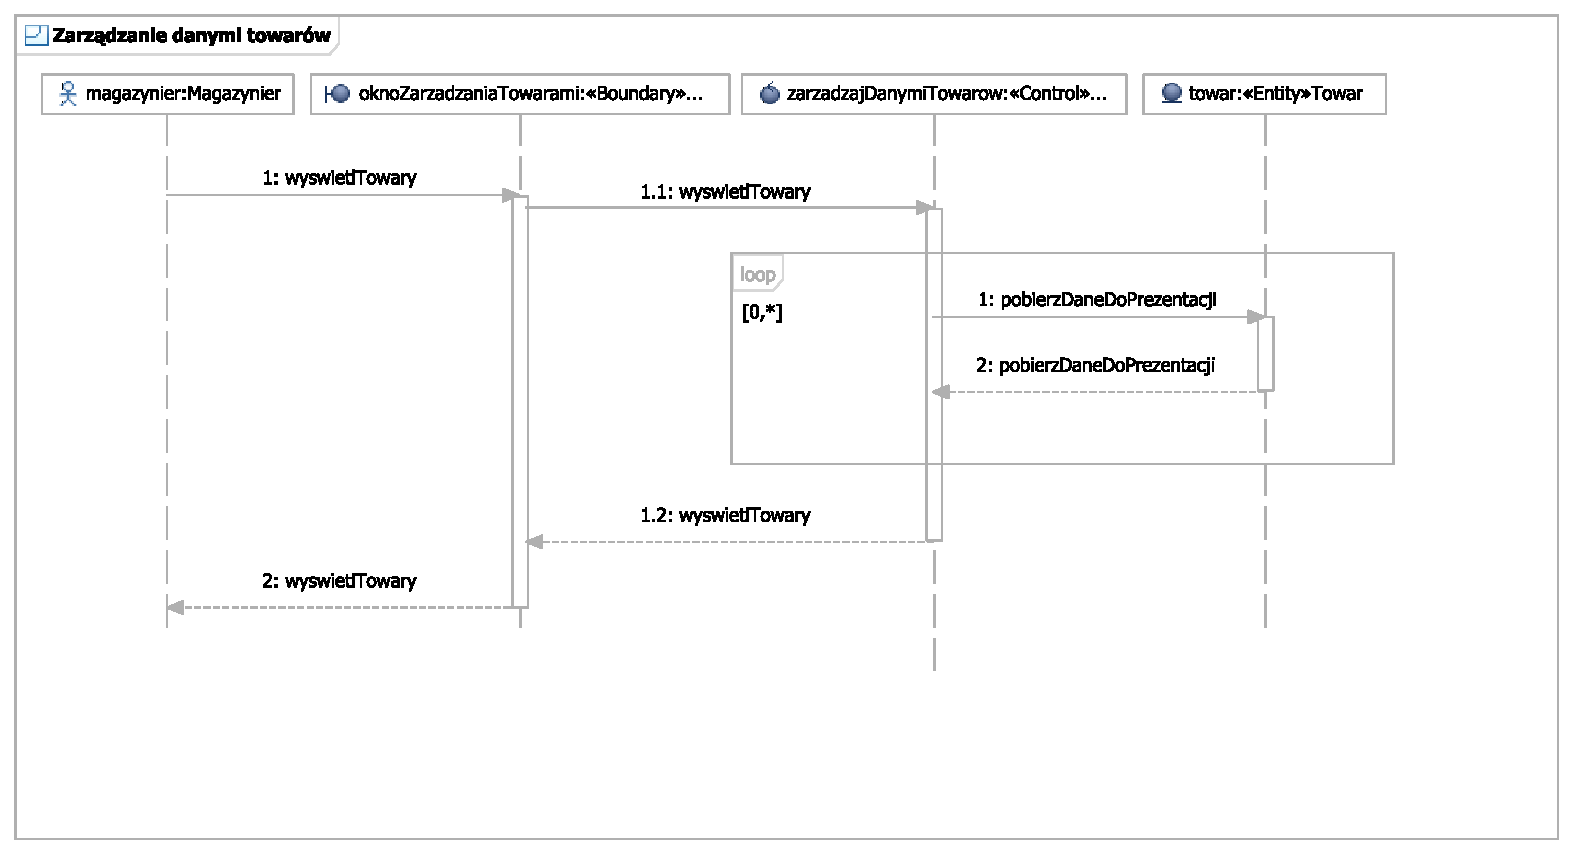
\includegraphics[angle=\seqangle, scale=\seqscale]{../img/usecase/pu18seq.pdf}
  \caption{\seqcaption18}
\end{figure}
\newpage

%%%%%%%%
\subsection{Dodawanie towaru}
%
\begin{usecase}
  \addtitle{PU19}{Dodawanie towaru}
  \addfield{Priorytet:}{wysoki}
  \addfield{Aktor główny:}{Magazynier}
  \addfield{Rozszerza przypadki:}{PU18}
  \addfield{Warunki początkowe:}{Aktor został uwierzytelniony.}
  \additemizedfield{Warunki końcowe:}{ 
    \item Dane towaru zostały zapisane w systemie.
    \item Użytkownik może wyświetlić dane towaru na liście towarów. % TODO jak warunki końcowe mają się do scenariuszy alternatywnych?
    \item Dane towaru mogą być uwzględnione w dokumentach przedstawionych w rozdziale \ref{dziedzina-problemu}.
  }
  \addscenario{Scenariusz główny:}{
    \item Aktor wybiera opcję dodania nowego towaru do systemu.
    \item System wyświetla formularz dodawania nowego towaru do systemu.
    \item Aktor wpisuje wymagane oraz opcjonalne dane do formularza.
    \item Aktor wybiera opcję zapisania nowego towaru w systemie.
    \item System informuje aktora, że towar został poprawnie zapisany w systemie.
  }
  \addscenario{Scenariusz alternatywny:} {
    \item [4.a] Aktor nie podał wymaganych pól formularza:
      \begin{enumerate}
        \item[1--4.] Jak w scenariuszu głównym.
        \item[5.] System wyświetla powiadomienie o konieczności podania wymaganych informacji.
        \item[6.] Aktor wraca do punktu 3.  
      \end{enumerate}
    \item [4.b] Aktor podał błędne wartości pól formularza:
      \begin{enumerate}
        \item[1--4.] Jak w scenariuszu głównym.
        \item[5.] System wyświetla powiadomienie o błędnych polach formularza.
        \item[6.] Aktor wraca do punktu 3.
      \end{enumerate}
  }
  \addfield{Zakres przetwarzanych danych:} {
    Dane towaru takie jak przedstawione w rozdziale \ref{dziedzina-problemu}.
  }
  \addfield{Warunki poprawności danych:}{
    Warunki poprawności takie jak przedstawione w rozdziale \ref{dziedzina-problemu}.
  }
  \addfield{Wymagania funkcjonalne:}{2.1}
\end{usecase}

\begin{figure}[H]
  \centering
  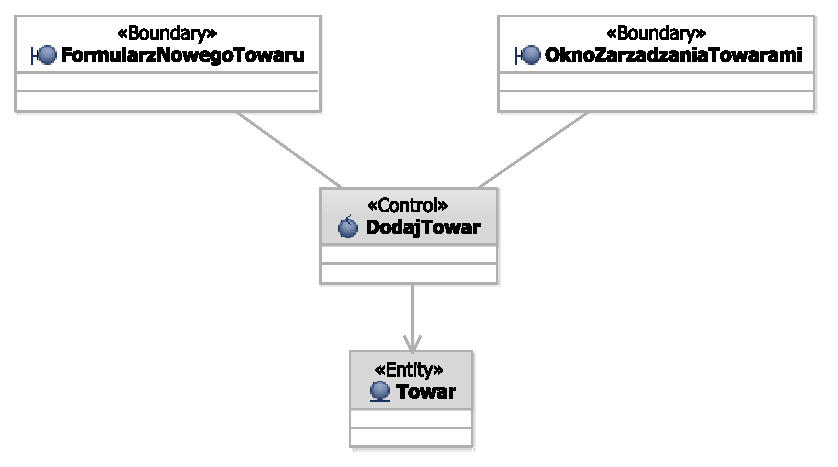
\includegraphics[angle=\ecbangle, scale=\ecbscale]{../img/usecase/pu19ecb.pdf}
  \caption{\ecbcaption19}
\end{figure}

\begin{figure}[H]
  \centering
  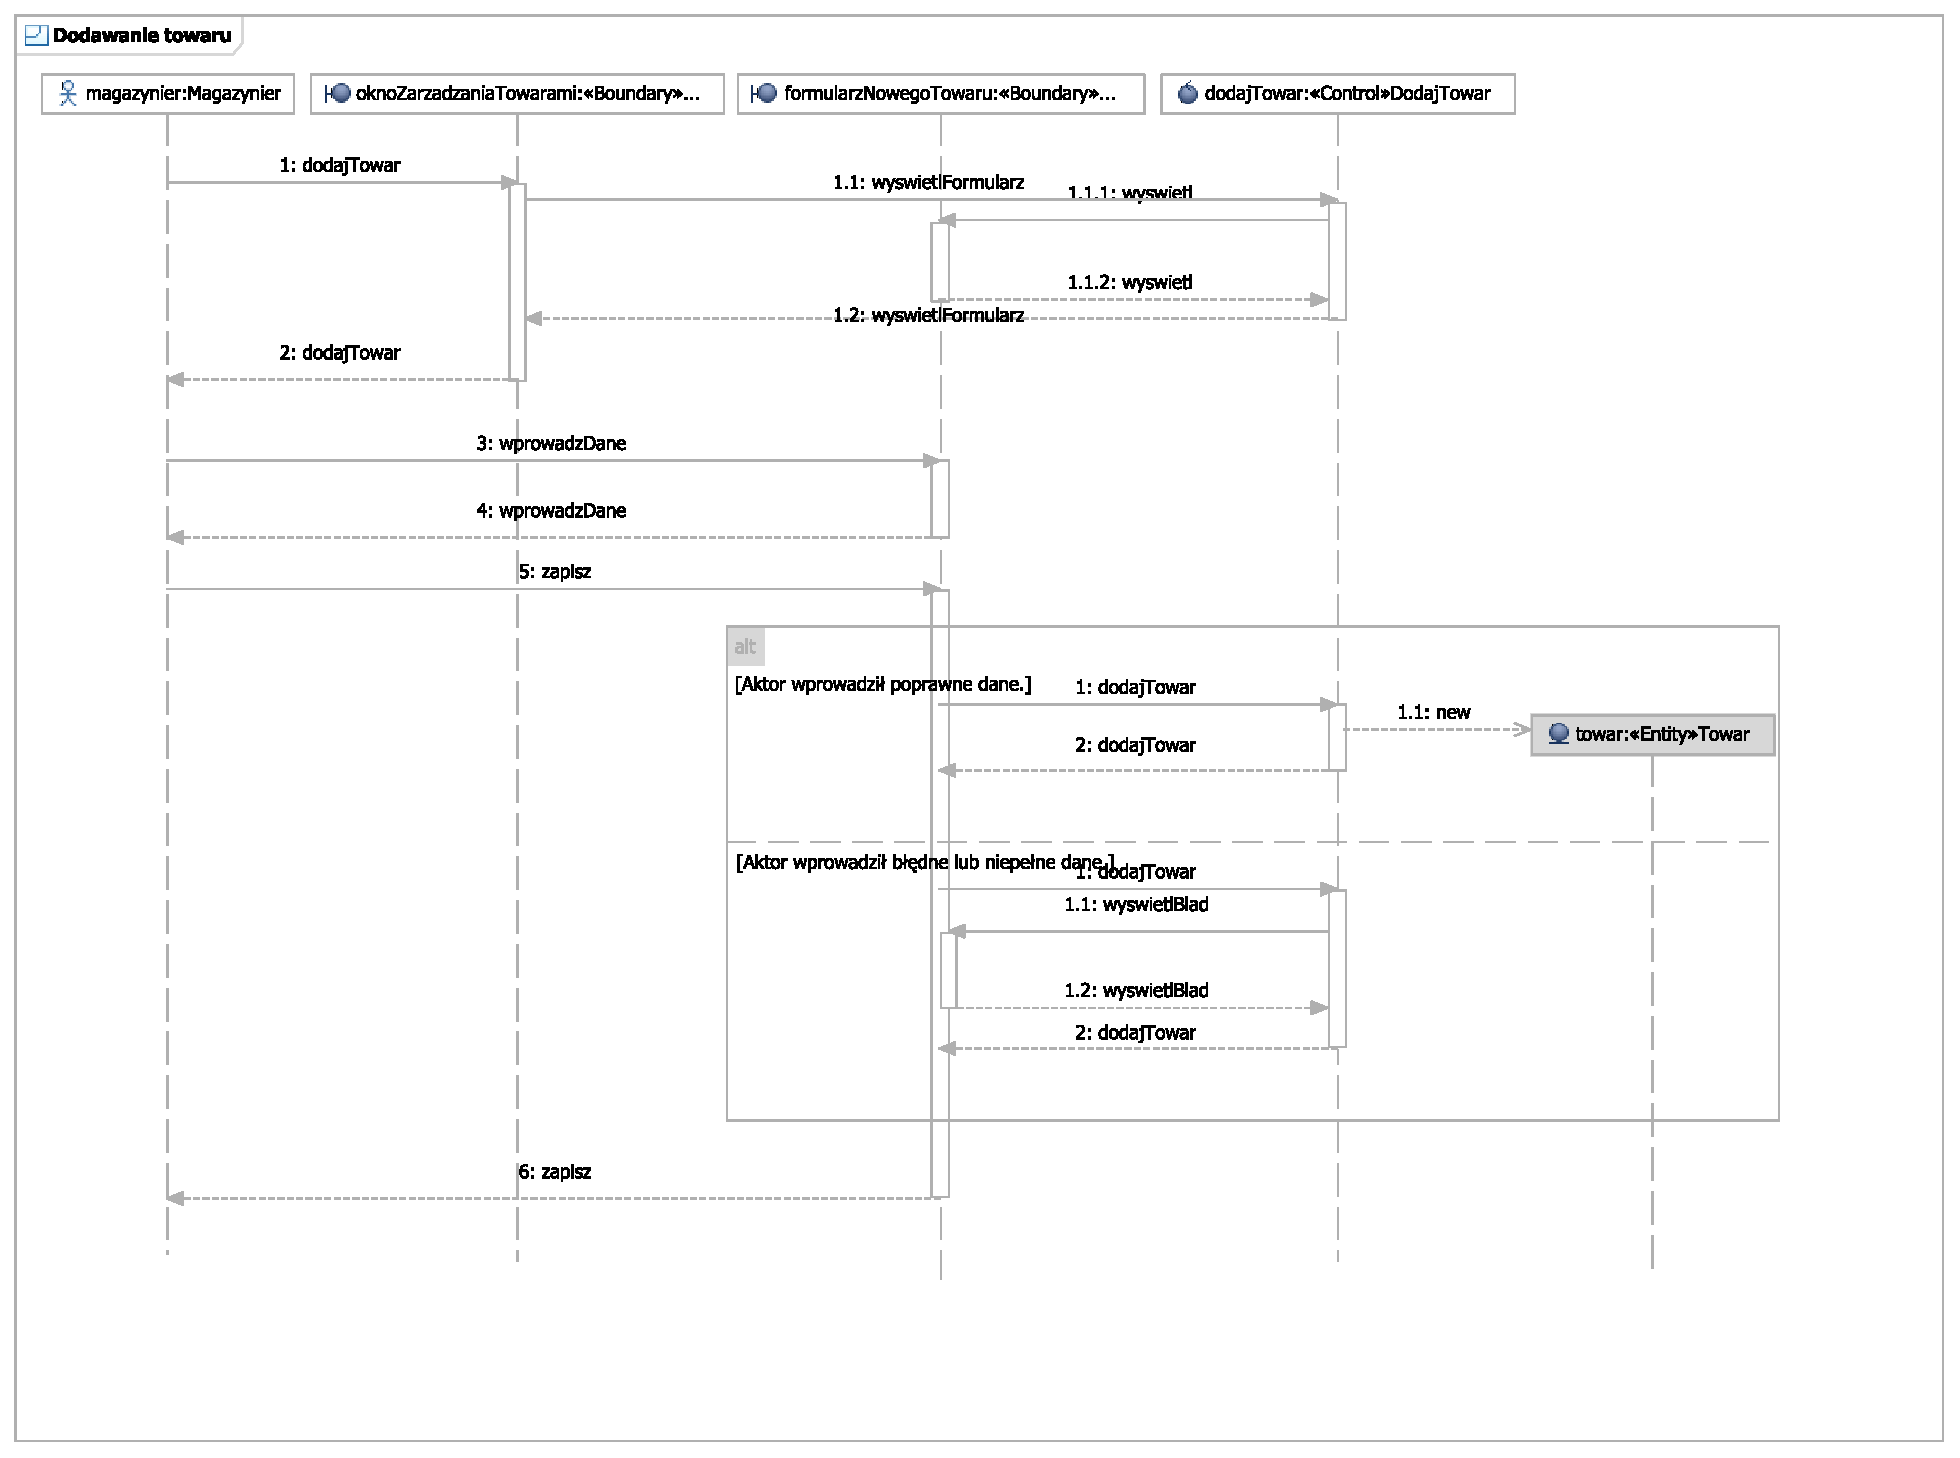
\includegraphics[angle=\seqangle, scale=0.5]{../img/usecase/pu19seq.pdf}
  \caption{\seqcaption19}
\end{figure}
\newpage

%%%%%%%
\subsection{Edycja opisu towaru}
\begin{usecase}
  \addtitle{PU20}{Edycja opisu towaru}
  \addfield{Priorytet:}{wysoki}
  \addfield{Aktor główny:}{Magazynier}
  \addfield{Rozszerza przypadki:}{PU18}
  \addfield{Warunki początkowe:}{Aktor został uwierzytelniony.}
   \additemizedfield{Warunki końcowe:}{ 
    \item Dane towaru zostały zaktualizowane w systemie.
    \item Użytkownik może wyświetlić dane towaru na liście towarów. 
    \item Dane towaru mogą być uwzględnione w dokumentach przedstawionych w rozdziale \ref{dziedzina-problemu}.
  }
  \addscenario{Scenariusz główny:}{
    \item Aktor wybiera opcję aktualizacji danych wskazanego towaru.
    \item System wyświetla formularz aktualizacji danych towaru wypełniony obecnymi danymi towaru.
    \item Aktor wypełnia lub zmienia wybrane pola formularza.
    \item Aktor wybiera opcję aktualizacji danych towaru.
    \item System informuje aktora, że dane towaru zostały poprawnie zaktualizowane.
  }
  % TODO duplikacja przebiegów alternatywnych z PU31
  \addscenario{Scenariusz alternatywny:} {
    \item [4.a] Aktor nie podał wymaganych pól formularza:
      \begin{enumerate}
        \item[1.--4.] Jak w scenariuszu głównym.
        \item[5.] System wyświetla powiadomienie o konieczności podania wymaganych informacji.
        \item[6.] Aktor wraca do punktu 3.  
      \end{enumerate}
    \item [4.b] Aktor podał błędne wartości pól formularza:
      \begin{enumerate}
        \item[1.--4.] Jak w scenariuszu głównym.
        \item[5.] System wyświetla powiadomienie o błędnych polach formularza.
        \item[6.] Aktor wraca do punktu 3.
      \end{enumerate}
  }
  \addfield{Zakres przetwarzanych danych:}{Dane towaru dostępne przy edycji, przedstawione w rozdziale \ref{dziedzina-problemu}.}
  \addfield{Warunki poprawności danych:}{Warunki poprawności takie jak przedstawione w rozdziale \ref{dziedzina-problemu}.}
  \addfield{Wymagania funkcjonalne:}{2.2}
\end{usecase}

\begin{figure}[H]
  \centering
  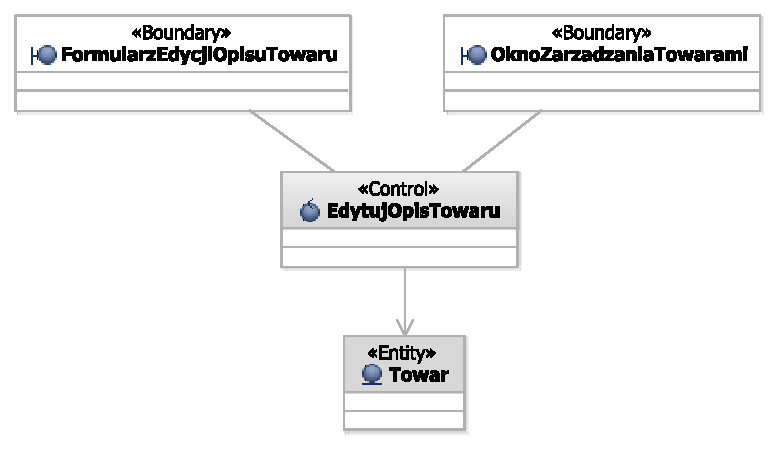
\includegraphics[angle=\ecbangle, scale=\ecbscale]{../img/usecase/pu20ecb.pdf}
  \caption{\ecbcaption20}
\end{figure}
\begin{figure}[H]
  \centering
  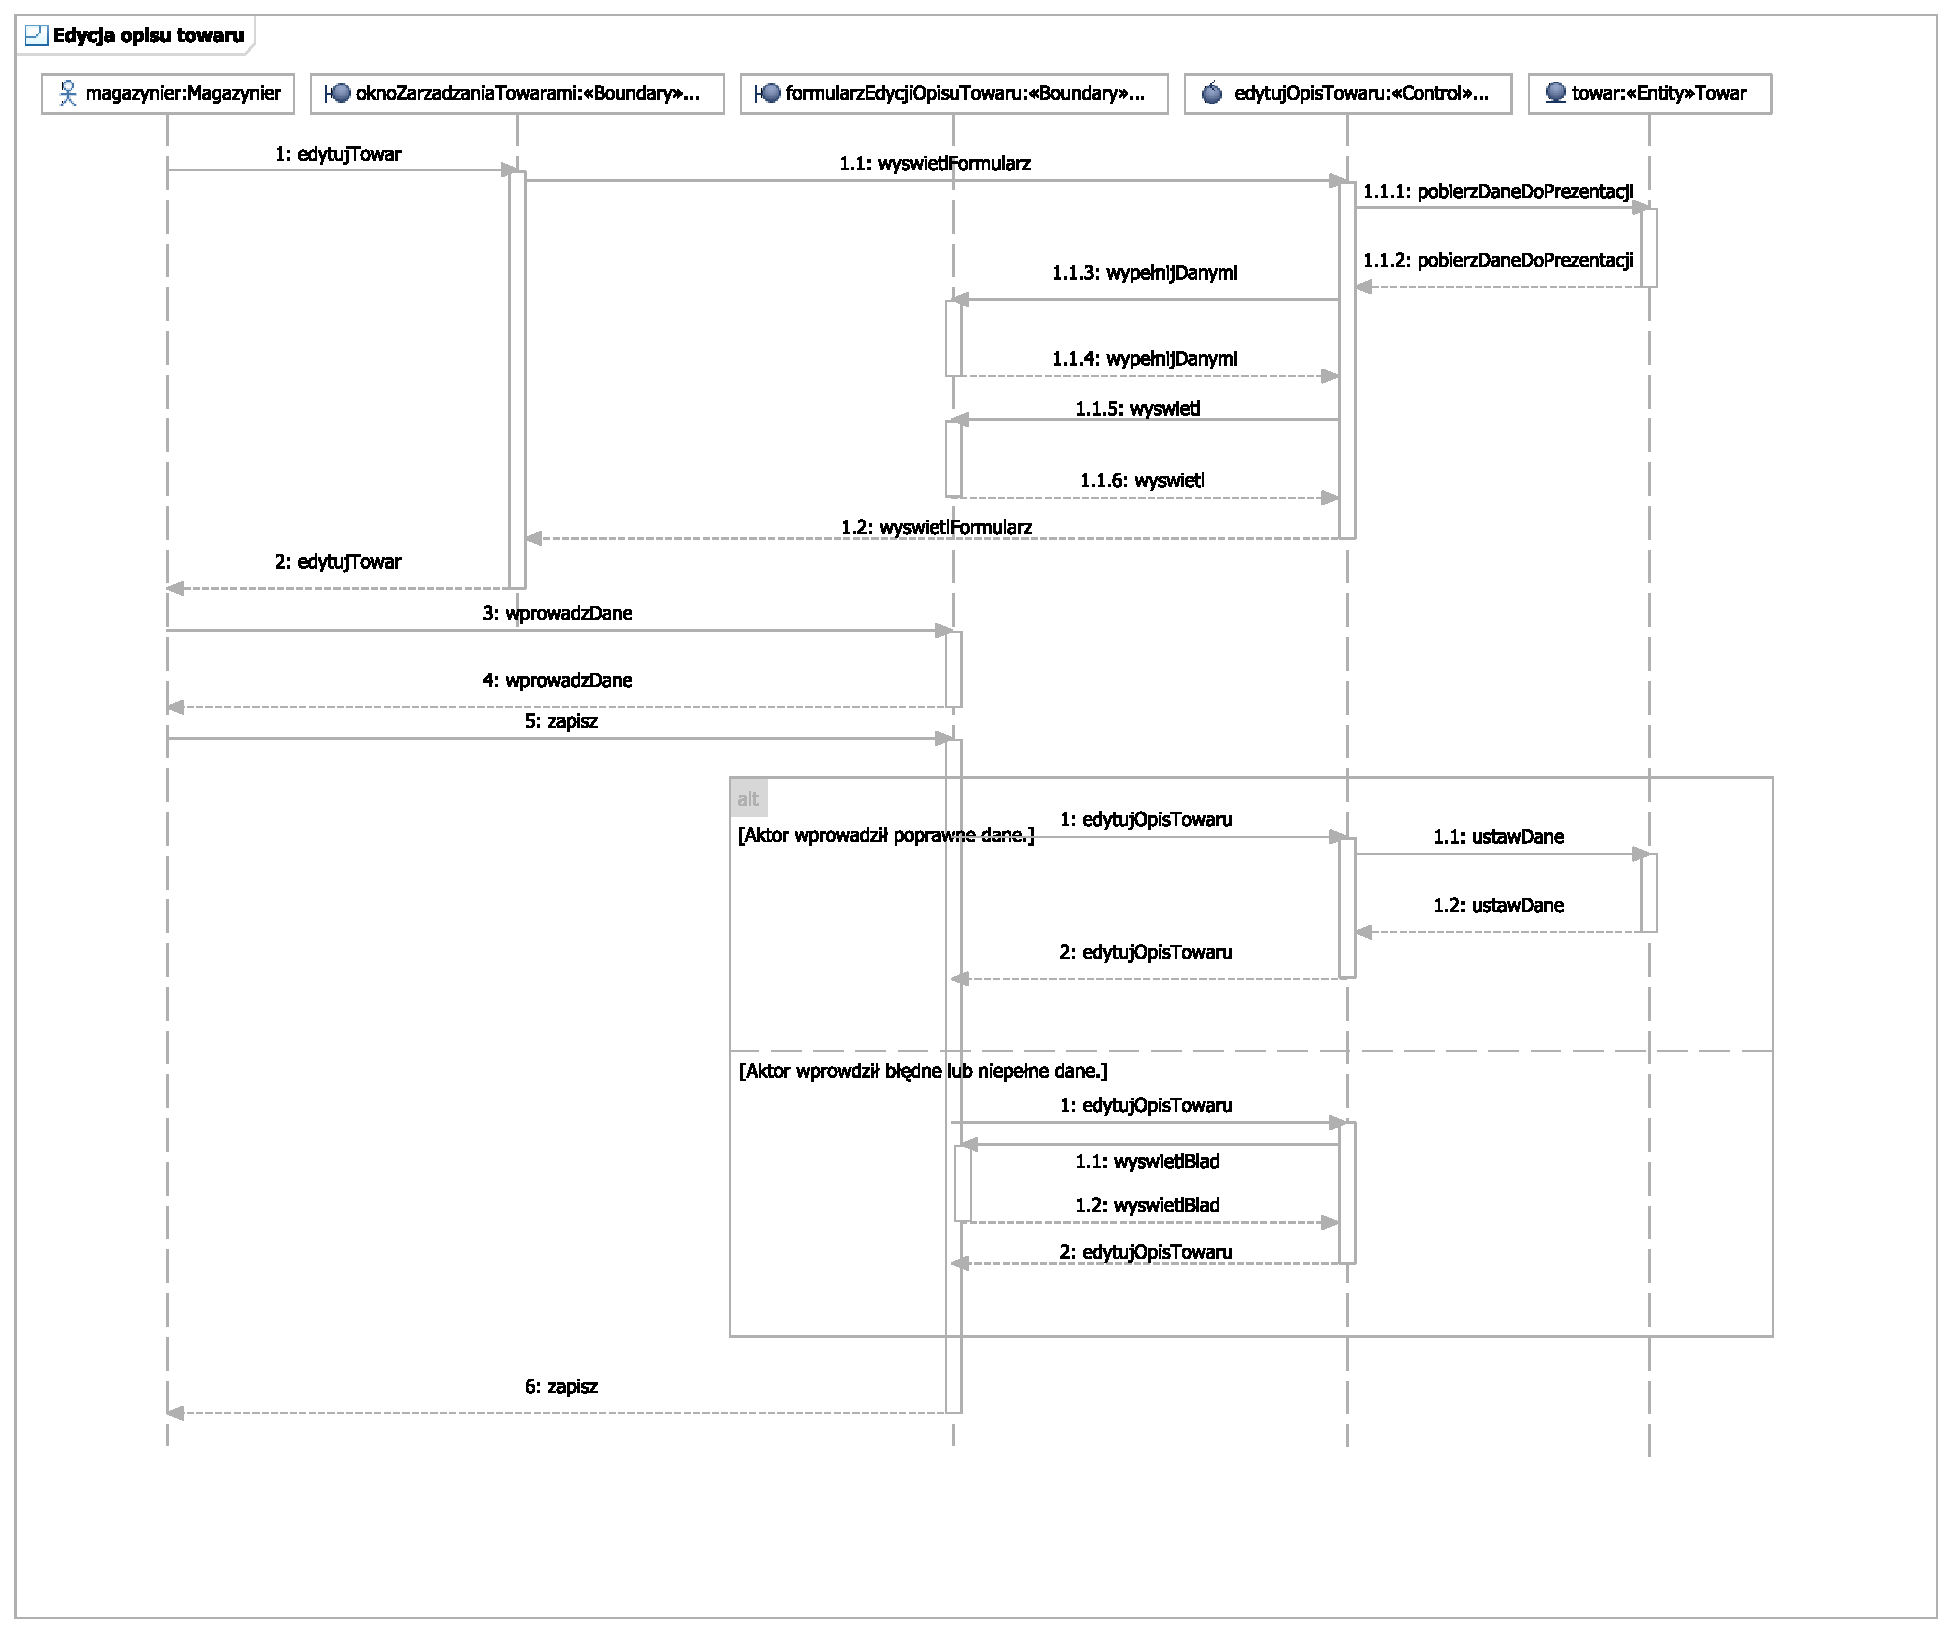
\includegraphics[angle=\seqangle, scale=0.45]{../img/usecase/pu20seq.pdf}
  \caption{\seqcaption20}
\end{figure}
\newpage

%%%%%%%
\subsection{Usuwanie danych towaru}
\begin{usecase}
  \addtitle{PU21}{Usuwanie danych towaru}
  \addfield{Priorytet:}{wysoki}
  \addfield{Aktor główny:}{Magazynier}
  \addfield{Rozszerza przypadki:}{PU18}
  \addfield{Warunki początkowe:}{Aktor został uwierzytelniony.}
  \additemizedfield{Warunki końcowe:}{
    \item Dane towaru zostały usunięte z systemu.
    \item Usunięty towar nie jest wypisywany na liście towarów w magazynie.
  }
  \addscenario{Scenariusz główny:}{
    \item Aktor wybiera opcję usunięcia danych towaru z systemu.
    \item System prosi o potwierdzenie operacji.
    \item Aktor potwierdza usunięcie towaru z systemu.
    \item System wyświetla informację o pomyślnym usunięciu towaru z systemu.
  }
  \addscenario{Scenariusz alternatywny:}{
    \item[4.a] Aktor anuluje usunięcie towaru z systemu.
      \begin{enumerate}
        \item[1.--2.] Jak w scenariuszu głównym.
        \item[3.] Aktor anuluje usunięcie towaru z systemu.
        \item[4.] System wyświetla informację, że operacja została anulowana.
      \end{enumerate}
  }
  \addfield{Wymagania funkcjonalne:}{2.3}
\end{usecase}

\begin{figure}[H]
  \centering
  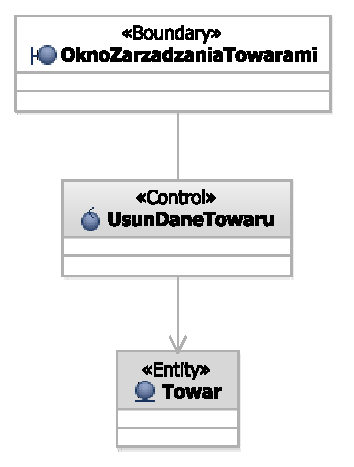
\includegraphics[angle=\ecbangle, scale=\ecbscale]{../img/usecase/pu21ecb.pdf}
  \caption{\ecbcaption21}
\end{figure}

\begin{figure}[H]
  \centering
  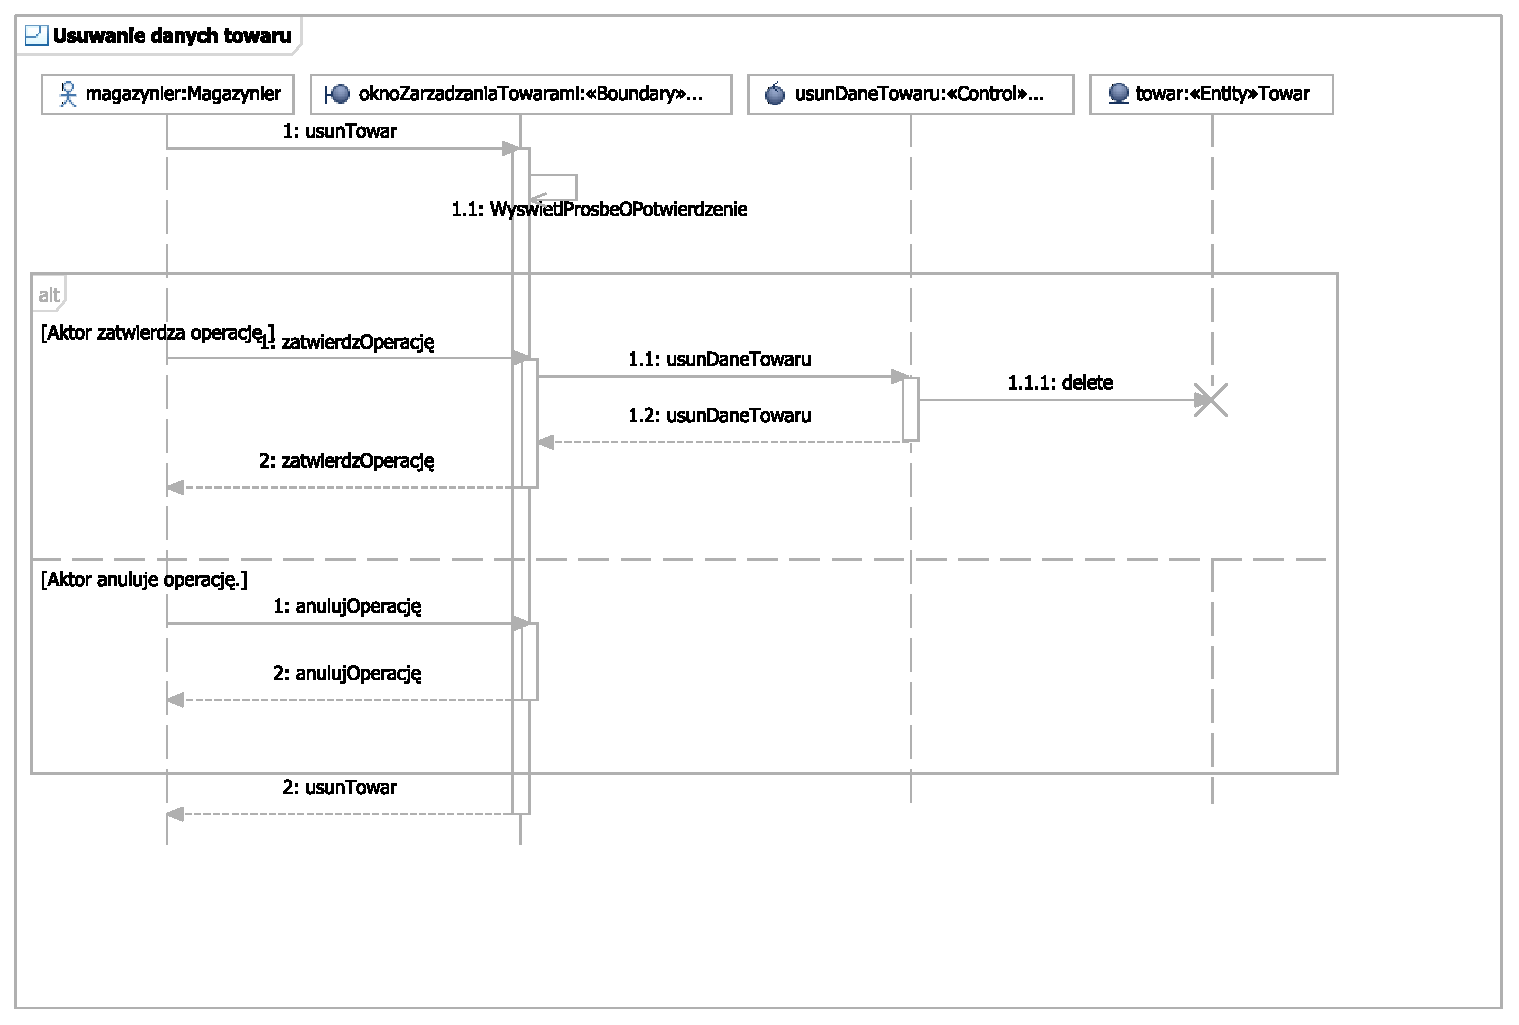
\includegraphics[angle=\seqangle, scale=\seqscale]{../img/usecase/pu21seq.pdf}
  \caption{\seqcaption21}
\end{figure}
\newpage

\subsection{Korekta stanu towarów}
\begin{usecase}
  \addtitle{PU22}{Korekta stanu towarów}
  \addfield{Priorytet:}{wysoki}
  \addfield{Aktor główny:}{Magazynier}
  \addfield{Rozszerza przypadki:}{PU18, PU20}
  \additemizedfield{Warunki początkowe:}{
    \item Aktor został uwierzytelniony.
    \item W systemie są zapisane dane co najmniej jednego towaru.
  }
  \additemizedfield{Warunki końcowe:} {
    \item Ilość towarów została zaktualizowana zgodnie z podaną wartością korekty oraz obecnym stanem towarów.
    \item Ilość każdego towaru przechowywana w systemie musi spełniać warunki poprawności przedstawione w \ref{dziedzina-problemu}.
    \item W systemie został zapisany dokument korekty stanu towarów w magazynie.
  }
  \addscenario{Scenariusz główny:}{
     \item Aktor wybiera opcję utworzenia dokumentu korekty stanu towarów.
     \item System wyświetla formularz korekty stanu towarów.
     \item Aktor wypełnia podstawowe dane dokumentu.
     \item Aktor wybiera towary, których stan podlega korekcie w tworzonym dokumencie oraz podaje ich nowe ilości.
     \item Aktor wybiera opcję zapisania dokumentu.
     \item System informuje aktora, że dane zostały poprawnie zaktualizowane.
  }
  \addscenario{Scenariusz alternatywny:} {
     \item[3.a] Aktor podał niepoprawne dane.
       \begin{enumerate}
          \item[1--3.] Jak w scenariuszu głównym.
          \item[4.] System informuje aktora, że podana wartość nie jest prawidłowa.
          \item[5.] Aktor wraca do punktu 3.
       \end{enumerate}
     \item[4.a] Aktor wybrał ten sam towar co najmniej dwa razy.
       \begin{enumerate}
       \item[1--4.] Jak w scenariuszu głównym.
       \item[5.] System informuje aktora, że co najmniej dwa razy wybrał ten sam towar, podane ilości towaru zostaną więc zsumowane.
       \item[6.] System wyświetla zsumowane wartości dla tych samych towarów.
       \item[7--...] Jak w scenariuszu głównym.
       \end{enumerate}
  }
  \addfield{Zakres przetwarzanych danych:} {
    Dane wprowadzane zgodne z informacjami przedstawionymi w \ref{dziedzina-problemu}.
  }
  \addfield{Warunki poprawności danych:} {
    Takie jak przedstawione w \ref{dziedzina-problemu}.
  }
  \addfield{Wymagania funkcjonalne:}{2.2.2}
\end{usecase}

\begin{figure}[H]
  \centering
  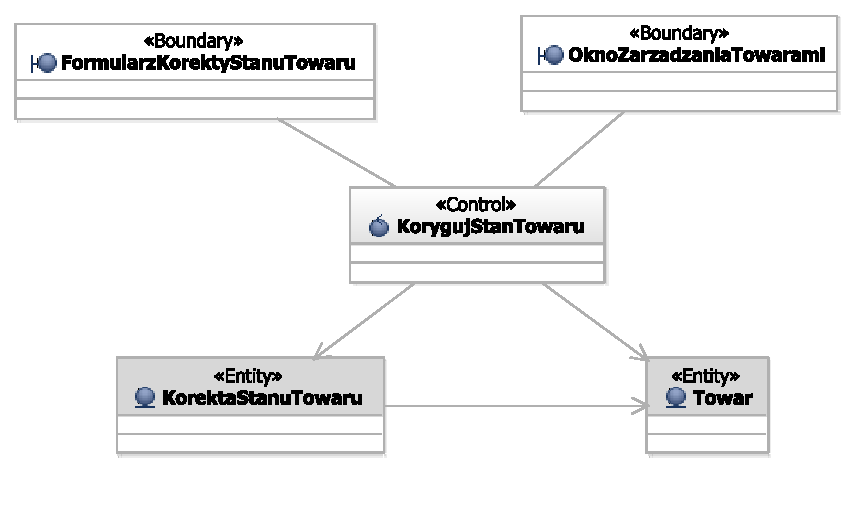
\includegraphics[angle=\ecbangle, scale=\ecbscale]{../img/usecase/pu22ecb.pdf}
  \caption{\ecbcaption22}
\end{figure}
\newpage
\begin{figure}[H]
  \centering
  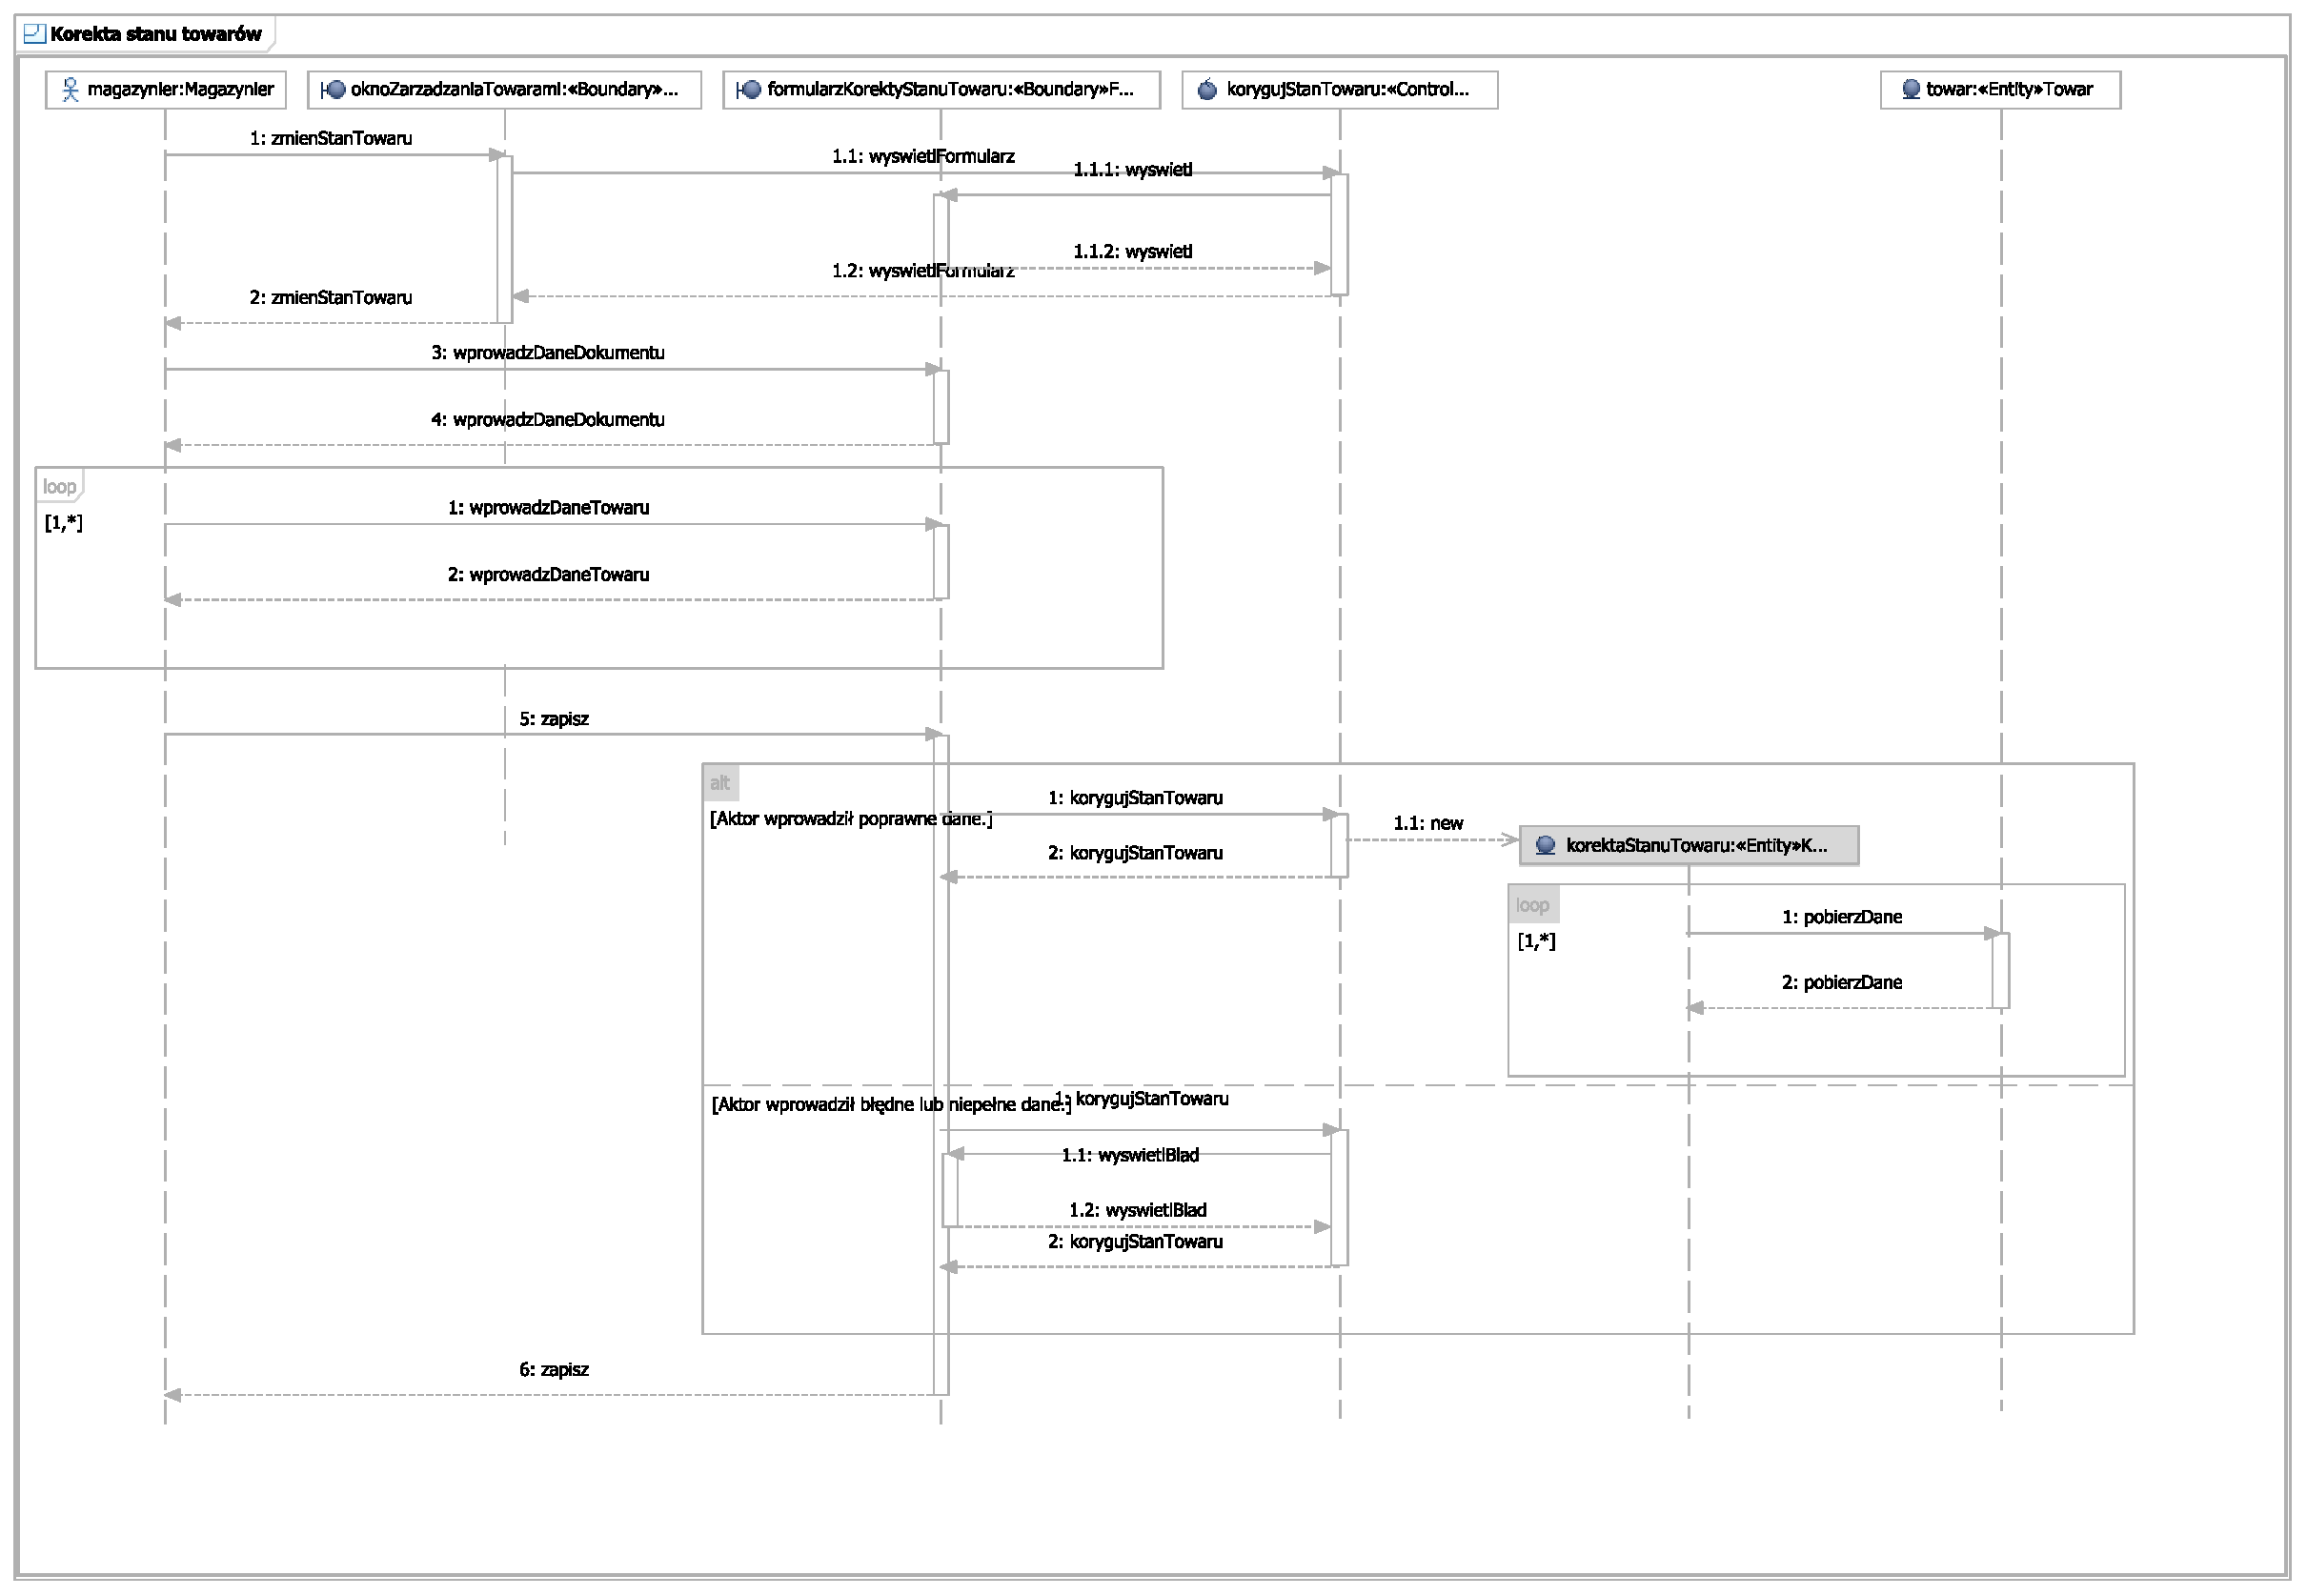
\includegraphics[angle=\seqangle, scale=0.40]{../img/usecase/pu22seq.pdf}
  \caption{\seqcaption22}
\end{figure}
\newpage

% %%%%%%
\subsection{Przyjęcie towaru na magazyn}
\begin{usecase}
  \addtitle{PU23}{Przyjęcie towaru na magazyn}
  \addfield{Priorytet:}{wysoki}
  \addfield{Aktor główny:}{Magazynier}
  \addfield{Warunki początkowe:}{Aktor został uwierzytelniony.}
  % Warunki końcowe (brak).
  \addscenario{Scenariusz główny:}{
  \item Aktor wybiera opcję przyjęcia towaru na magazyn.
  \item System wyświetla listę dokumentów PZ wraz z opcjami do zarządzania dokumentami przyjęcia towaru.
  }
  \addfield{Wymagania funkcjonalne:}{4.}
\end{usecase}

\begin{figure}[H]
  \centering
  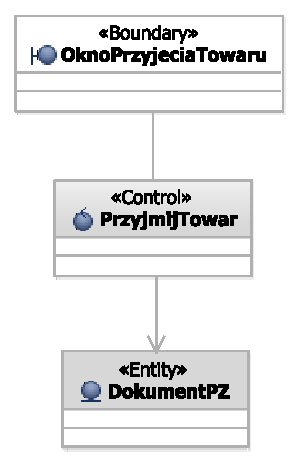
\includegraphics[angle=\ecbangle, scale=\ecbscale]{../img/usecase/pu23ecb.pdf}
  \caption{\ecbcaption23}
\end{figure}
\newpage
\begin{figure}[H]
  \centering
  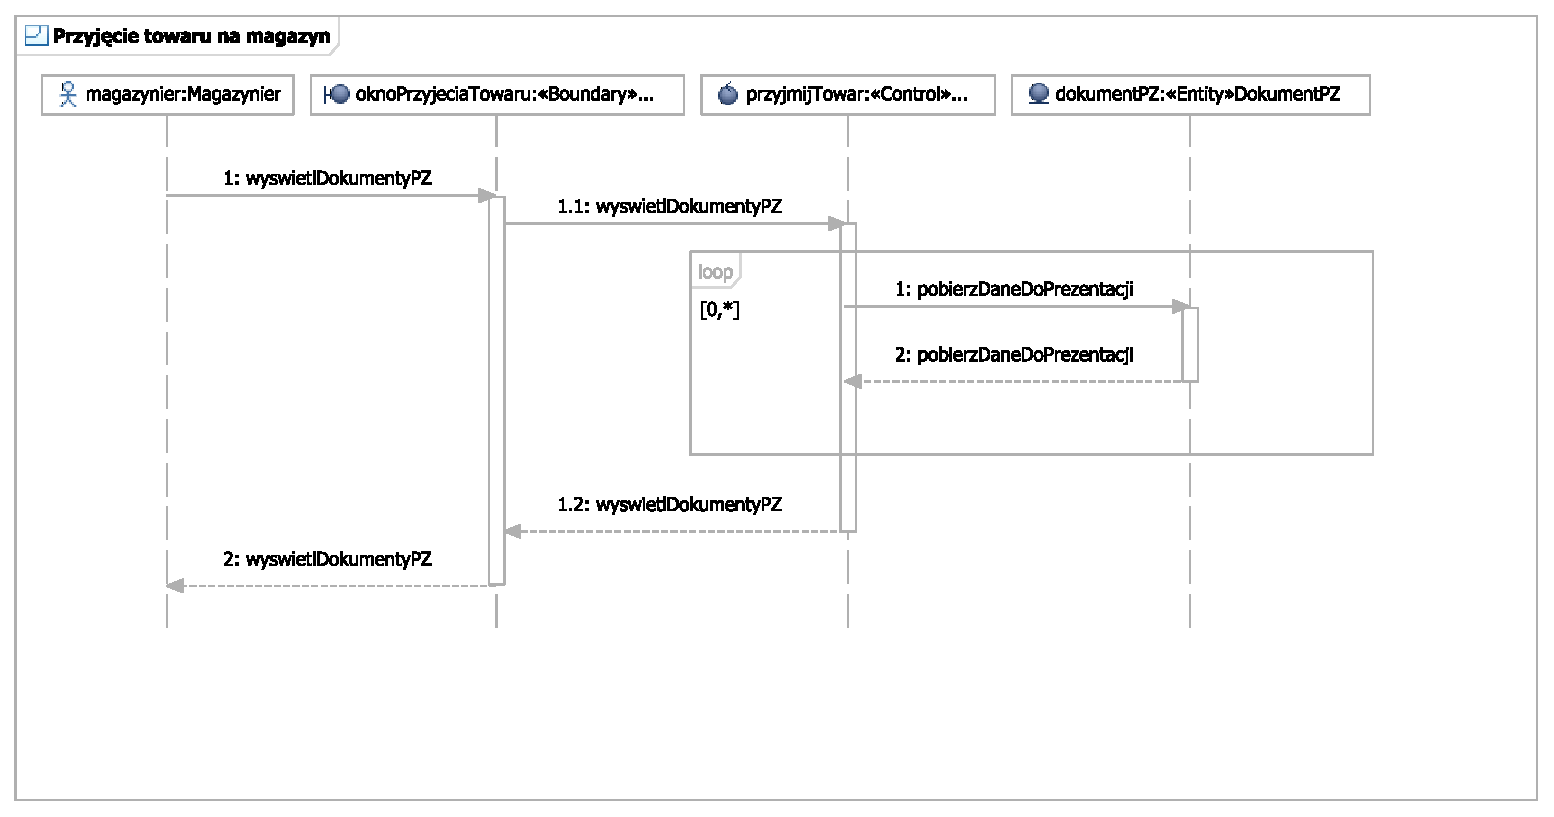
\includegraphics[angle=\seqangle, scale=\seqscale]{../img/usecase/pu23seq.pdf}
  \caption{\seqcaption23}
\end{figure}
\newpage

%%%%%%%
\subsection{Tworzenie dokumentu przyjęcia towaru}
\begin{usecase}
  \addtitle{PU24}{Tworzenie dokumentu przyjęcia towaru}
  \addfield{Priorytet:}{wysoki}
  \addfield{Aktor główny:}{Magazynier}
  \addfield{Rozszerza przypadki:}{PU23}
  \addfield{Warunki początkowe:}{Aktor został uwierzytelniony.}
  \additemizedfield{Warunki końcowe:}{ 
    \item Dokument przyjęcia towaru został zapisany w systemie.
    \item Aktor otrzymuje informacje o poprawnym dodaniu dokumentu do systemu.
    \item Użytkownik może wyświetlić dokument na liście dokumentów przyjęcia towaru. 
    \item Ilość przechowywanego towaru została zaktualizowana o ilość towaru zapisanego w dokumencie przyjęcia towaru.
    \item Ilość przechowywanego towaru jest zgodna z warunkami poprawności danych przedstawionymi w \ref{dziedzina-problemu}.
  }
  \addscenario{Scenariusz główny:}{
    \item Aktor wybiera opcję utworzenia nowego dokumentu przyjęcia towaru.
    \item System wyświetla formularz nowego dokumentu przyjęcia towaru.
    \item Aktor wypełnia podstawowe dane dokumentu.
    \item Aktor wybiera kontrahenta operacji.
    \item Aktor wybiera towary, które będą przyjęte od kontrahenta.
    \item Aktor wskazuje ilość oraz cenę jednostkową przyjmowanego towaru.
    \item Aktor wybiera opcję zapisania dokumentu.
    \item System informuje aktora, że dane zostały poprawnie zaktualizowane.
  }
  \addscenario{Scenariusz alternatywny:} {
    \item [3.a] Aktor nie podał wymaganych pól formularza:
      \begin{enumerate}
        \item[1--4.] Jak w scenariuszu głównym.
        \item[5.] System wyświetla powiadomienie o konieczności podania wymaganych informacji.
        \item[6.] Aktor wraca do punktu 3.  
      \end{enumerate}
    \item [3.b] Aktor podał błędne wartości pól formularza:
      \begin{enumerate}
        \item[1--4.] Jak w scenariuszu głównym.
        \item[5.] System wyświetla powiadomienie o błędnych polach formularza.
        \item[6.] Aktor wraca do punktu 3.
      \end{enumerate}
     \item[5.a] Aktor wybrał ten sam towar co najmniej dwa razy.
       \begin{enumerate}
       \item[1--5.] Jak w scenariuszu głównym.
       \item[6.] System informuje aktora, że co najmniej dwa razy wybrał ten sam towar, podane ilości towaru zostaną więc zsumowane.
       \item[7.] System wyświetla zsumowane wartości dla tych samych towarów.
       \item[8--...] Jak w scenariuszu głównym.
       \end{enumerate}
  }
  \addfield{Zakres przetwarzanych danych:} {
    Pola dokumentu przyjęcia towaru takie jak przedstawione w rozdziale \ref{dziedzina-problemu}.
  }
  \addfield{Warunki poprawności danych:}{
    Warunki poprawności takie jak przedstawione w rozdziale \ref{dziedzina-problemu}.
  }
  \addfield{Wymagania funkcjonalne:}{4.1}
\end{usecase}

\begin{figure}[H]
  \centering
  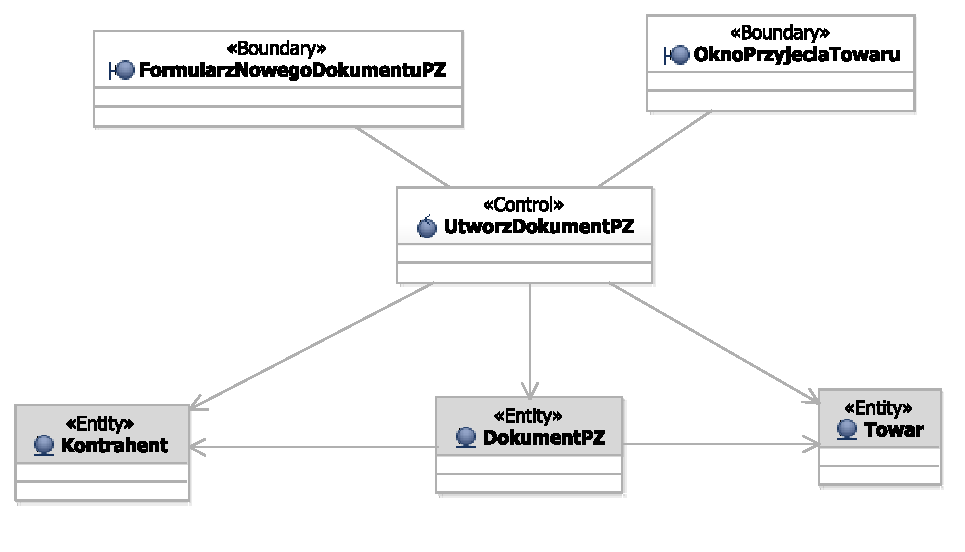
\includegraphics[angle=\ecbangle, scale=\ecbscale]{../img/usecase/pu24ecb.pdf}
  \caption{\ecbcaption24}
\end{figure}
\newpage
\begin{figure}[H]
  \centering
  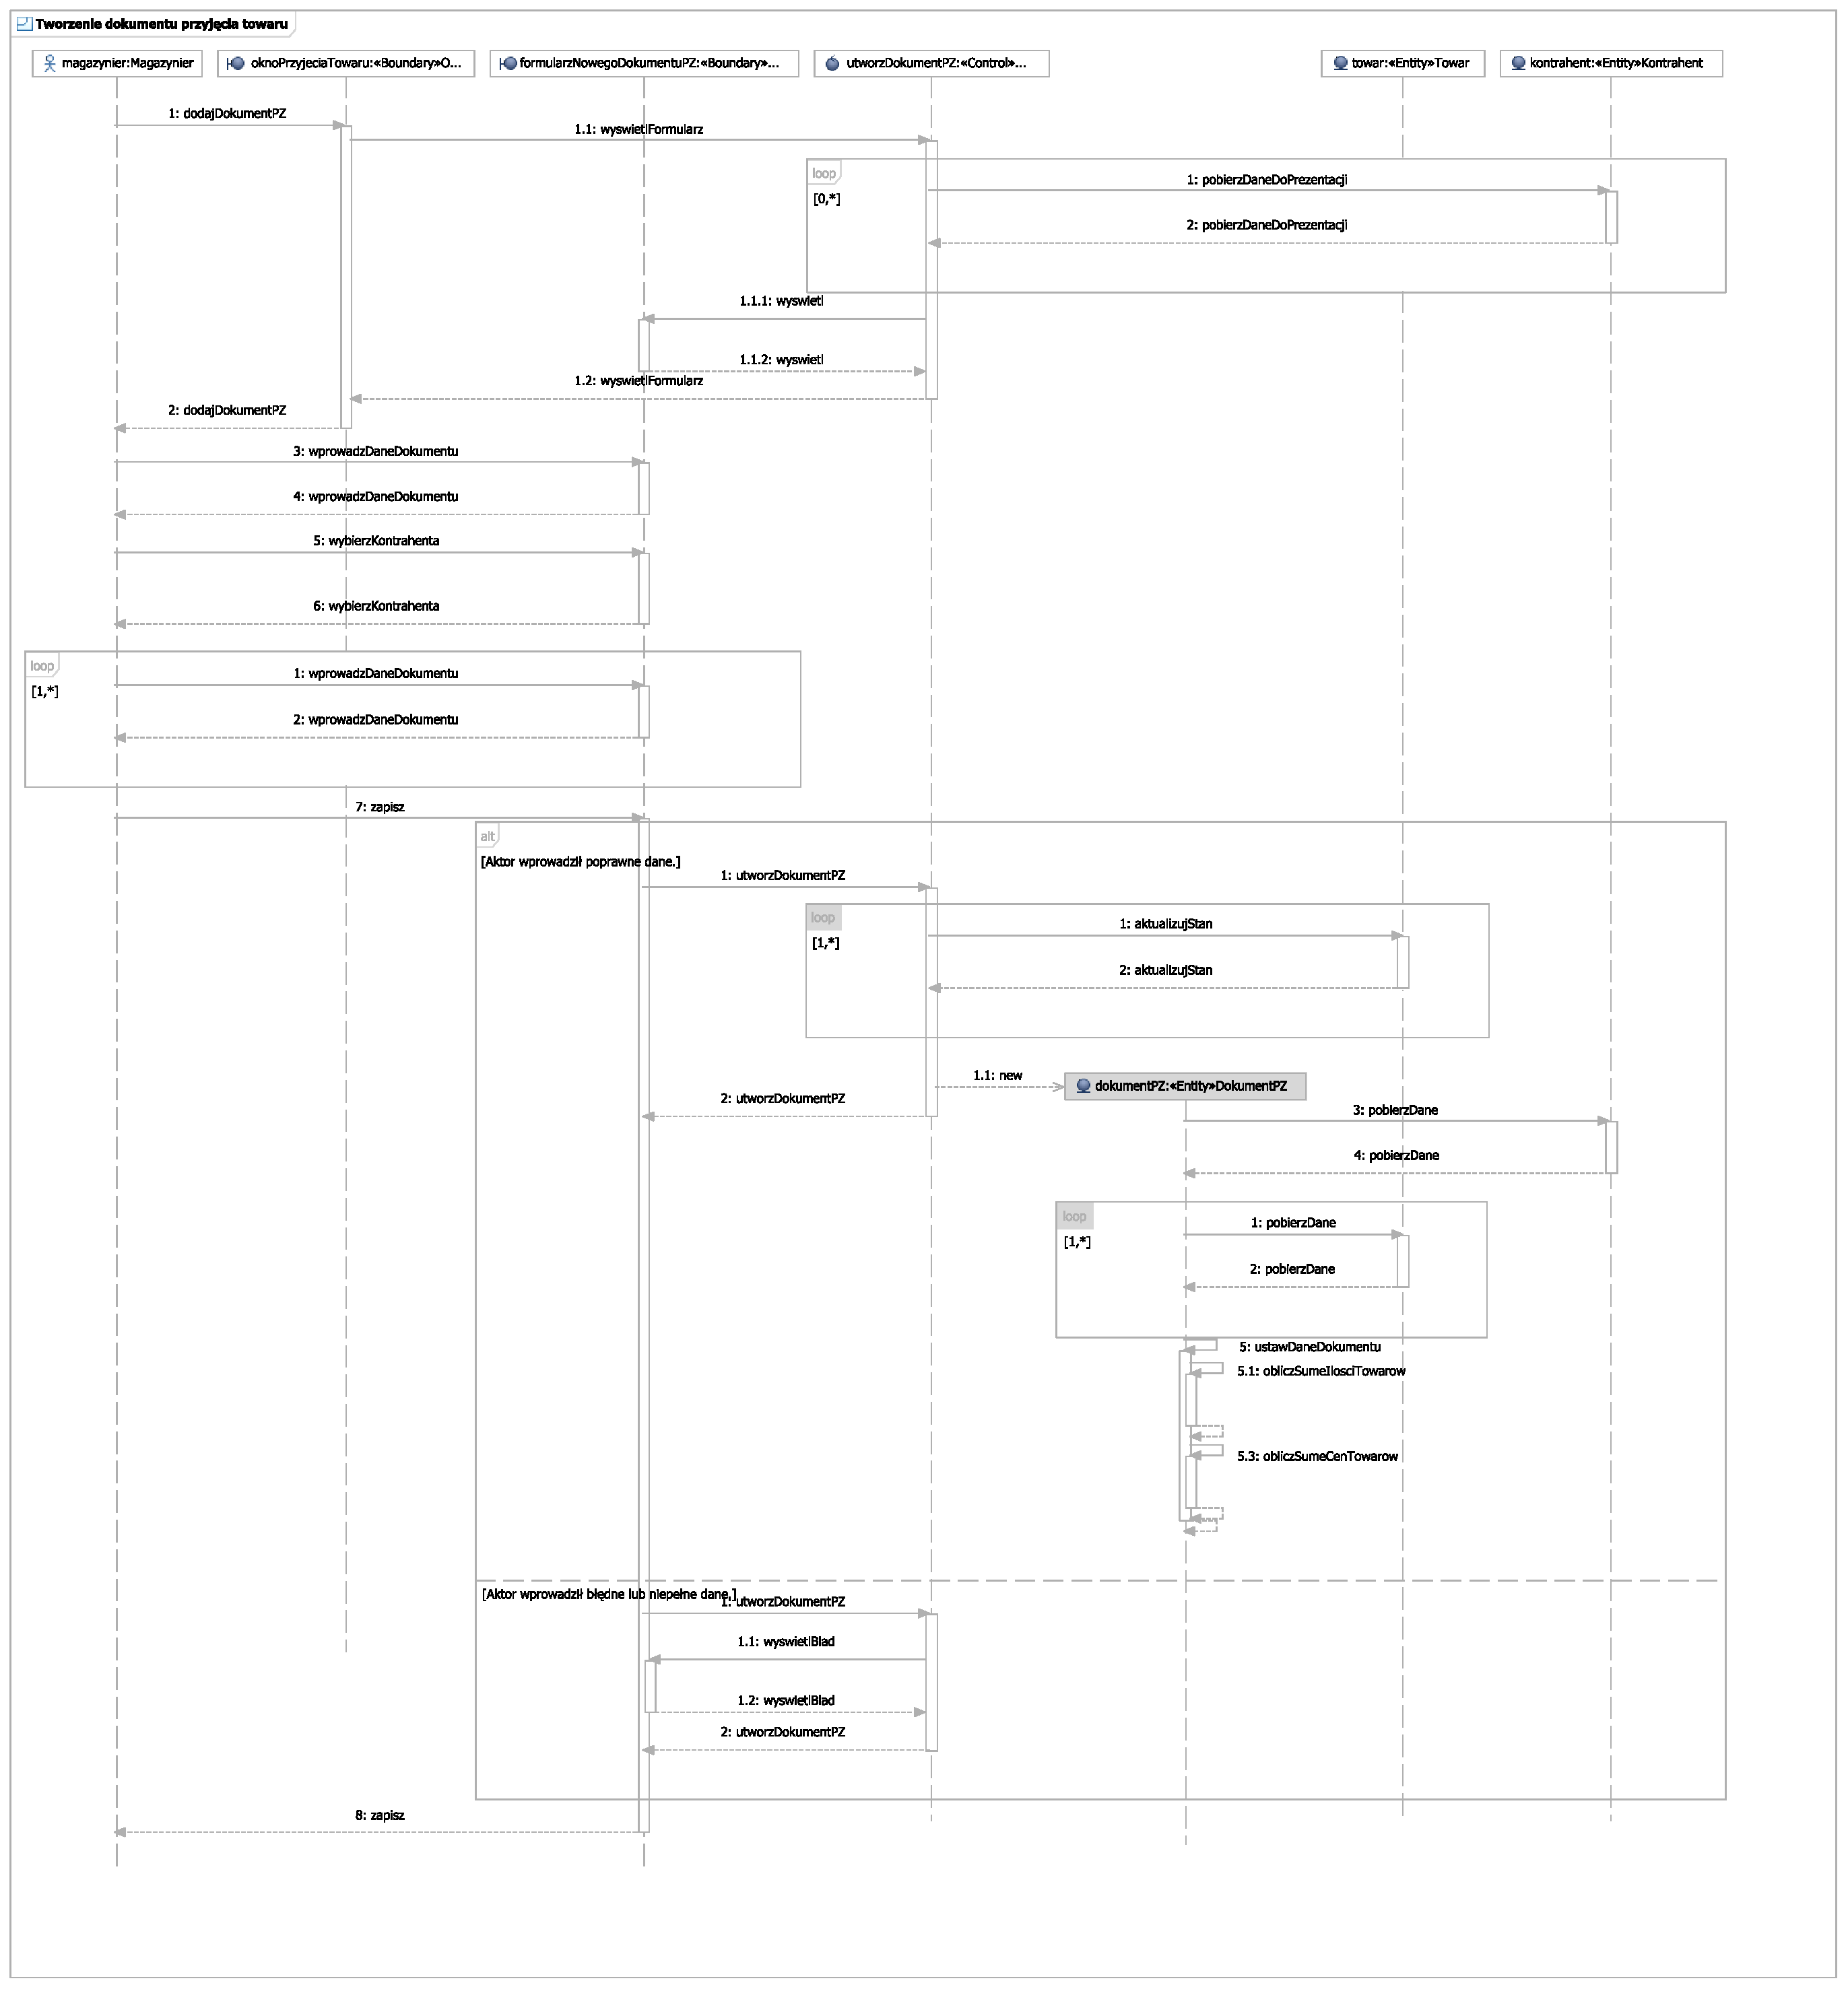
\includegraphics[angle=\seqangle, scale=0.35]{../img/usecase/pu24seq.pdf}
  \caption{\seqcaption24}
\end{figure}
\newpage

%%%%%%%%
\subsection{Edycja dokumentu przyjęcia towaru}
\begin{usecase}
  \addtitle{PU25}{Edycja dokumentu przyjęcia towaru}
  \addfield{Priorytet:}{wysoki}
  \addfield{Aktor główny:}{Magazynier}
  \addfield{Rozszerza przypadki:}{PU23}
  \additemizedfield{Warunki początkowe:}{
    \item Aktor został uwierzytelniony.
    \item Operacja przyjęcia towaru, którego dotyczy wybrany dokument, nie została jeszcze zrealizowana.
  }
  \additemizedfield{Warunki końcowe:}{ 
    \item Dane dokumentu zostały zaktualizowane w systemie.
    \item Użytkownik może wyświetlić dane dokumentu na liście dokumentów przyjęcia towaru. 
    \item Ilość przechowywanego towaru została zaktualizowana o ilość towaru zapisanego w dokumencie przyjęcia towaru.
    \item Ilość przechowywanego towaru jest zgodna z warunkami poprawności danych przedstawionymi w \ref{dziedzina-problemu}.
  }
  % TODO prawie duplikacja z Tworzeniem dokumentu przyjęcia towaru
  \addscenario{Scenariusz główny:}{
    \item Aktor wybiera opcję edycji wybranego dokumentu przyjęcia towaru.
    \item System wyświetla formularz edycji dokumentu przyjęcia towaru.
    \item Aktor wypełnia podstawowe dane dokumentu (oprócz pól wykluczonych z edycji).
    \item Aktor aktualizuje listę towarów, ich ilości oraz ceny jednostkowe.
    \item Aktor wybiera opcję aktualizacji dokumentu.
    \item System informuje aktora, że dane zostały poprawnie zaktualizowane.
  }
  \addscenario{Scenariusz alternatywny:} {
    \item [3.a] Aktor nie podał wymaganych pól formularza:
      \begin{enumerate}
        \item[1--4.] Jak w scenariuszu głównym.
        \item[5.] System wyświetla powiadomienie o konieczności podania wymaganych informacji.
        \item[6.] Aktor wraca do punktu 3.  
      \end{enumerate}
    \item [3.b] Aktor podał błędne wartości pól formularza:
      \begin{enumerate}
        \item[1--4.] Jak w scenariuszu głównym.
        \item[5.] System wyświetla powiadomienie o błędnych polach formularza.
        \item[6.] Aktor wraca do punktu 3.
      \end{enumerate}
     \item[4.a] Aktor wybrał ten sam towar co najmniej dwa razy.
       \begin{enumerate}
       \item[1--4.] Jak w scenariuszu głównym.
       \item[5.] System informuje aktora, że co najmniej dwa razy wybrał ten sam towar, podane ilości towaru zostaną więc zsumowane.
       \item[6.] System wyświetla zsumowane wartości dla tych samych towarów.
       \item[7--...] Jak w scenariuszu głównym.
       \end{enumerate}
  }
  \addfield{Zakres przetwarzanych danych:} {
    Pola dokumentu przyjęcia towaru takie jak przedstawione w rozdziale \ref{dziedzina-problemu}.
  }
  \addfield{Warunki poprawności danych:}{
    Warunki poprawności takie jak przedstawione w rozdziale \ref{dziedzina-problemu}.
  }
  \addfield{Wymagania funkcjonalne:}{4.2}
\end{usecase}

\begin{figure}[H]
  \centering
  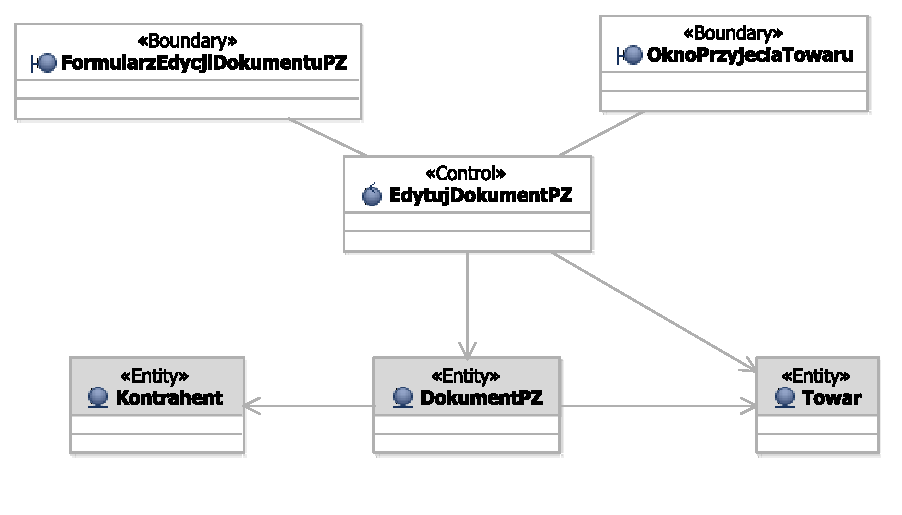
\includegraphics[angle=\ecbangle, scale=\ecbscale]{../img/usecase/pu25ecb.pdf}
  \caption{\ecbcaption25}
\end{figure}
\newpage
\begin{figure}[H]
  \centering
  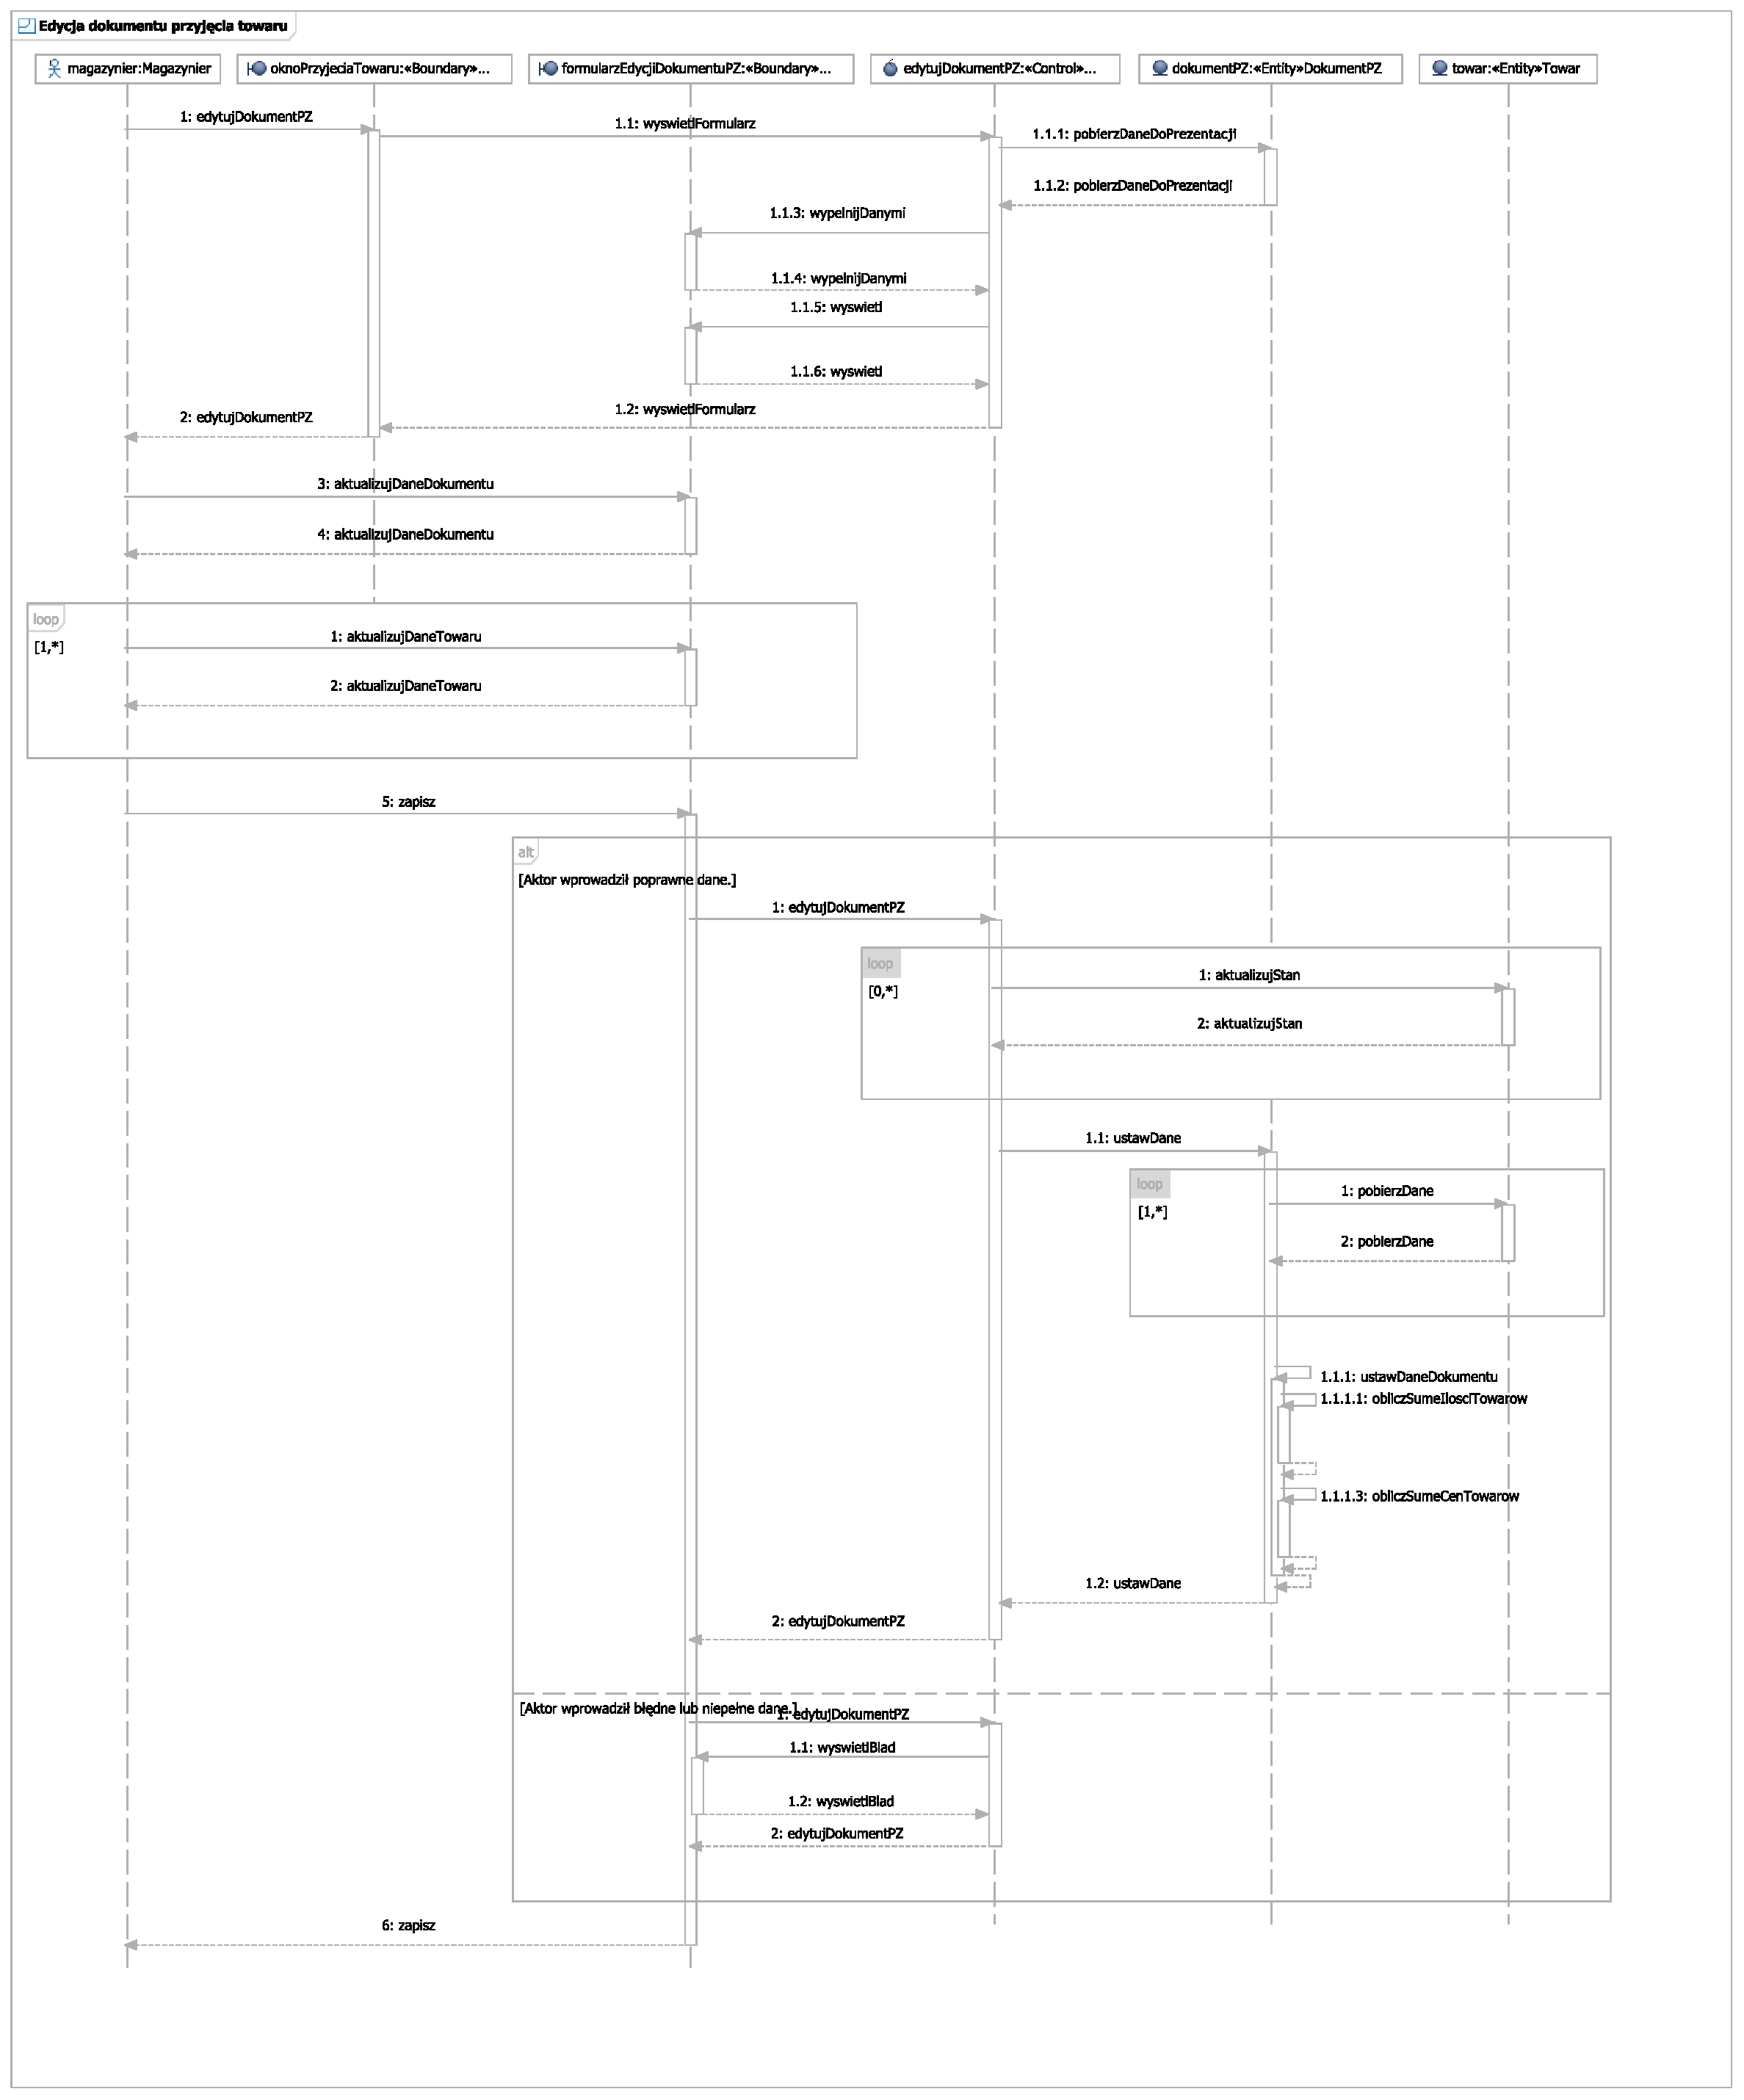
\includegraphics[angle=\seqangle, scale=\seqscalemin]{../img/usecase/pu25seq.pdf}
  \caption{\seqcaption25}
\end{figure}
\newpage

\subsection{Usuwanie dokumentu przyjęcia towaru}
\begin{usecase}
  \addtitle{PU26}{Usuwanie dokumentu przyjęcia towaru}
  \addfield{Priorytet:}{wysoki}
  \addfield{Aktor główny:}{Magazynier}
  \addfield{Rozszerza przypadki:}{PU23}
  \addfield{Warunki początkowe:}{Aktor został uwierzytelniony.}
  \additemizedfield{Warunki końcowe:}{
    \item Dane dokumentu zostały usunięte z systemu.
    \item Usunięty dokument nie jest wypisywany na liście dokumentów przyjęcia towaru.
    \item Stan towarów z usuniętego dokumentu jest zaktualizowany o ilości zapisane w usuwanym dokumencie.
  }
  \addscenario{Scenariusz główny:}{
    \item Aktor wybiera opcję usunięcia dokumentu przyjęcia towaru z systemu.
    \item System prosi o potwierdzenie operacji.
    \item Aktor potwierdza usunięcie dokumentu z systemu.
    \item System wyświetla informację o pomyślnym usunięciu dokumentu z systemu.
  }
  \addscenario{Scenariusz alternatywny:}{
    \item[2.a] Aktor anuluje usunięcie dokumentu z systemu.
      \begin{enumerate}
        \item[1.--2.] Jak w scenariuszu głównym.
        \item[3.] Aktor anuluje usunięcie dokumentu z systemu.
        \item[4.] System wyświetla informację, że operacja została anulowana.
      \end{enumerate}
  }
  \addfield{Wymagania funkcjonalne:}{4.3}
\end{usecase}

\begin{figure}[H]
  \centering
  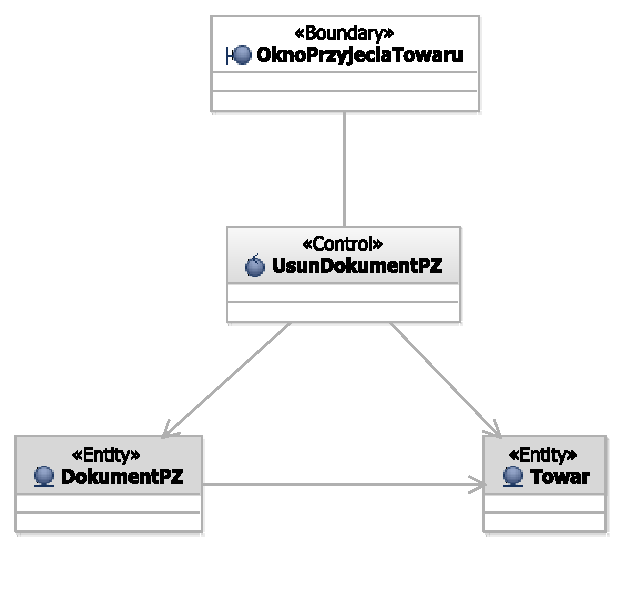
\includegraphics[angle=\ecbangle, scale=\ecbscale]{../img/usecase/pu26ecb.pdf}
  \caption{\ecbcaption26}
\end{figure}

\begin{figure}[H]
  \centering
  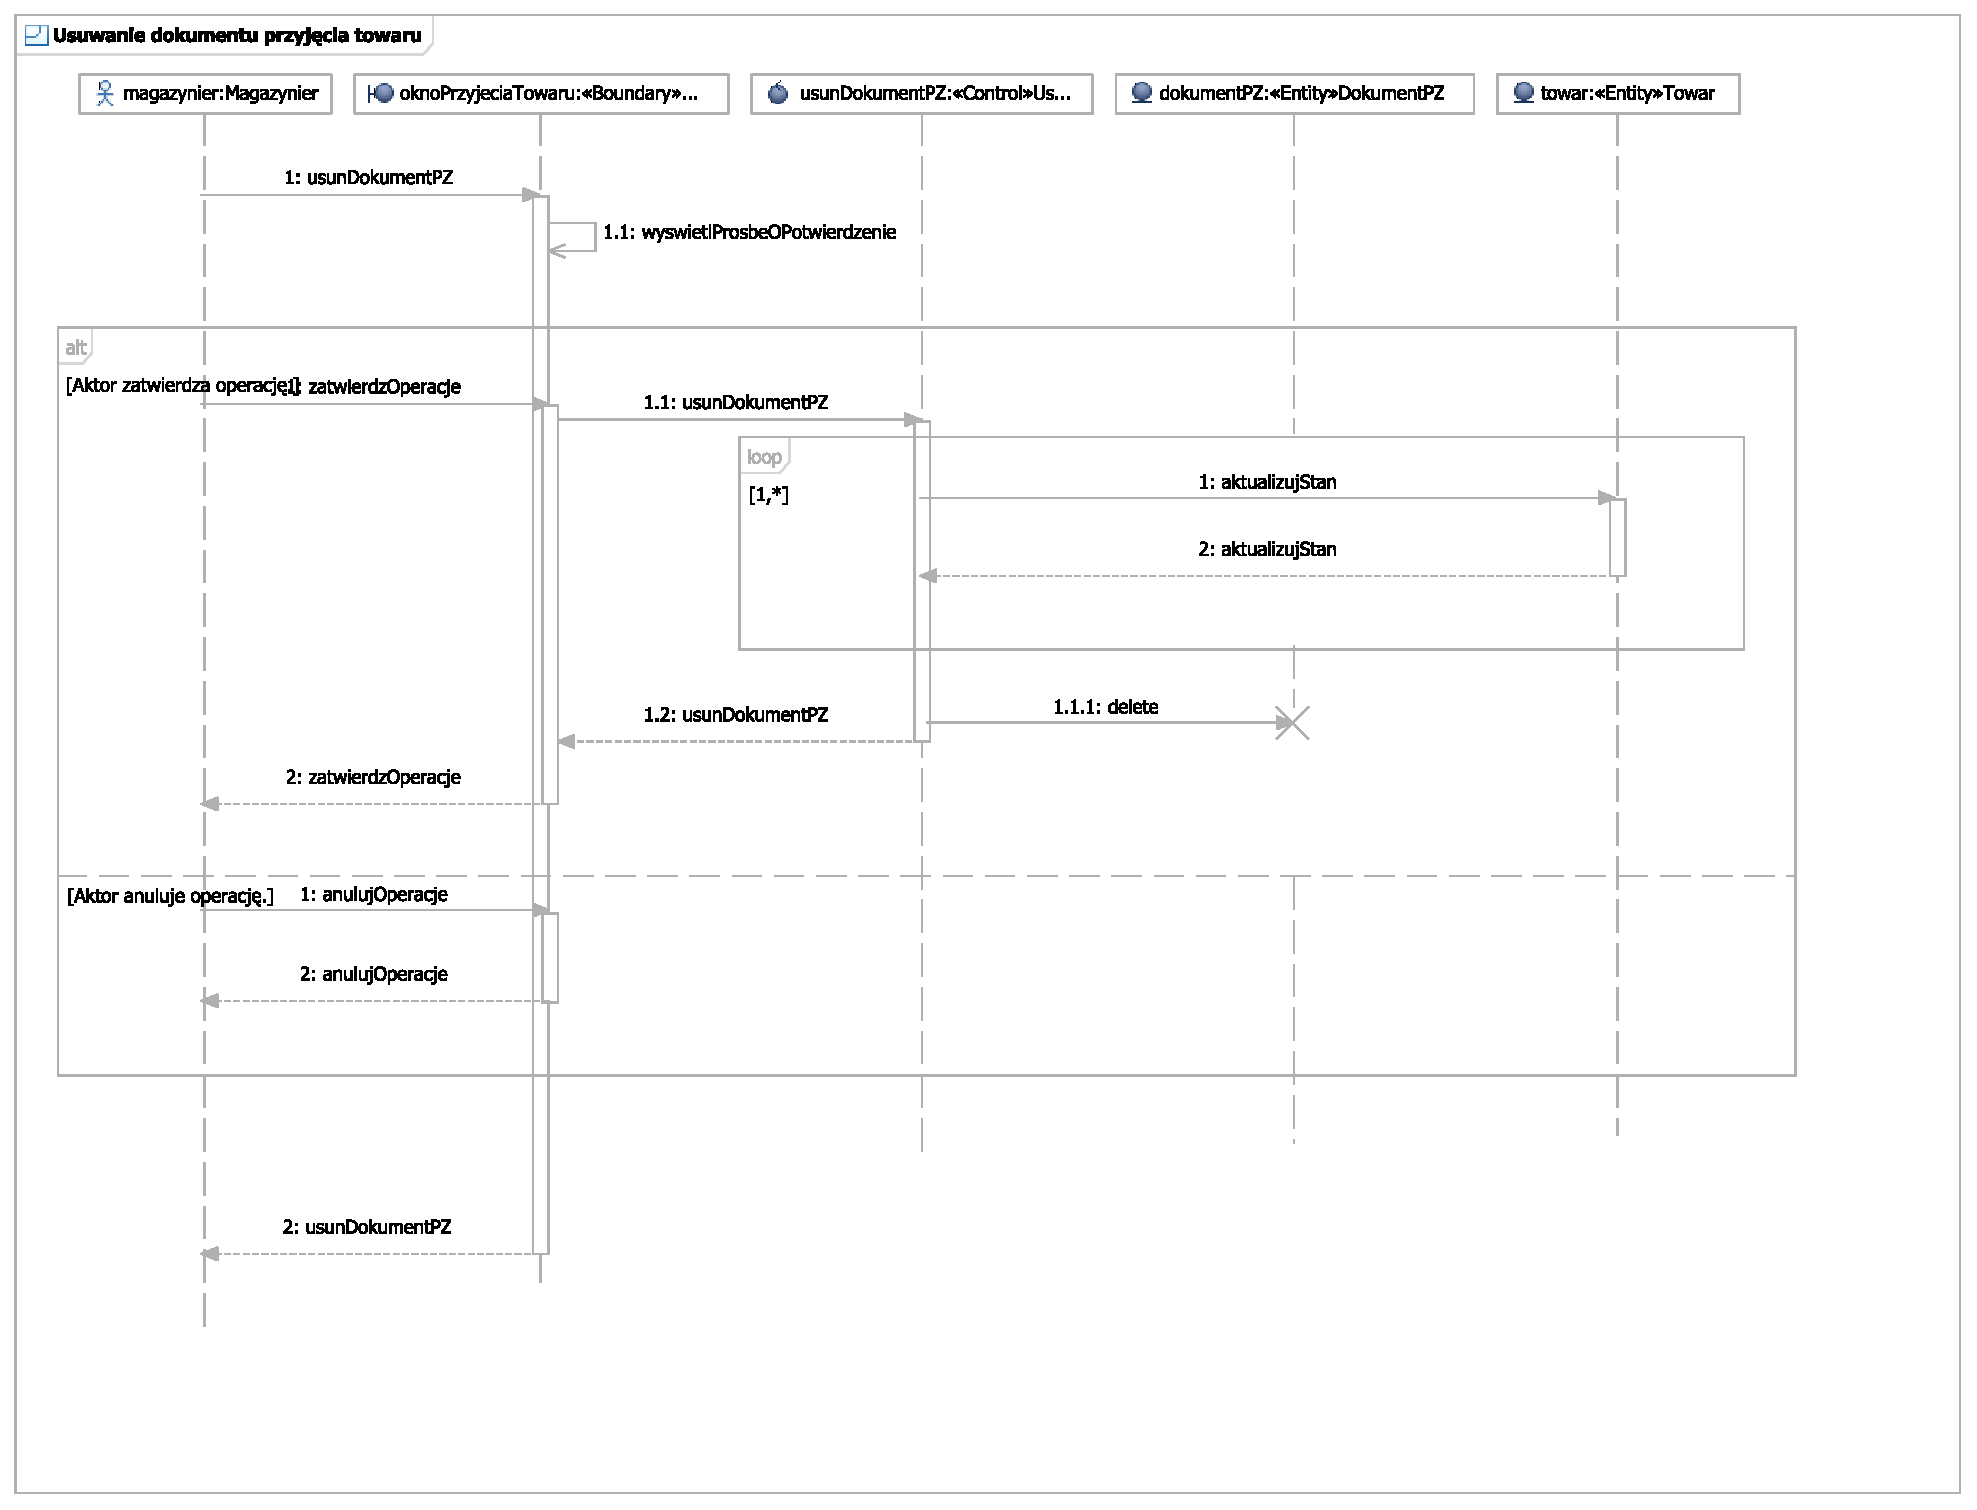
\includegraphics[angle=\seqangle, scale=0.5]{../img/usecase/pu26seq.pdf}
  \caption{\seqcaption26}
\end{figure}
\newpage

\subsection{Realizacja przyjęcia towaru na magazyn}
\begin{usecase}
  \addtitle{PU27}{Realizacja przyjęcia towaru na magazyn}
  \addfield{Priorytet:}{wysoki}
  \addfield{Aktor główny:}{Magazynier}
  \addfield{Rozszerza przypadki:}{PU23, PU24}
  \additemizedfield{Warunki początkowe:}{
    \item Aktor został uwierzytelniony.
    \item Wybrane przyjęcie towaru nie zostało jeszcze zrealizowane.}
  \additemizedfield{Warunki końcowe:} {
    \item Dokument przyjęcia towaru został oznaczony jako zrealizowany.
    \item Możliwe jest utworzenie korekty do zrealizowanego dokumentu przyjęcia towaru.
  }
  \addscenario{Scenariusz główny:}{
     \item Aktor wybiera opcję przyjęcia towaru na magazyn.
     \item System prosi o potwierdzenie realizacji przyjęcia towaru na magazyn.
     \item Aktor potwierdza realizację przyjęcia towaru na magazyn.
     % TODO mogło by być np powiadomienie dla dostawcy, że towar został przyjęty.
     \item System oznacza dokument przyjęcia towaru jako zrealizowany.
  }
 \addscenario{Scenariusz alternatywny:}{
    \item[4.a] Aktor anuluje realizację przyjęcia towaru.
      \begin{enumerate}
        \item[1.--2.] Jak w scenariuszu głównym.
        \item[3.] Aktor anuluje realizację dokumentu.
        \item[4.] System wyświetla informację, że operacja została anulowana.
      \end{enumerate}
  }
  \addfield{Wymagania funkcjonalne:}{4.4}
\end{usecase}

\begin{figure}[H]
  \centering
  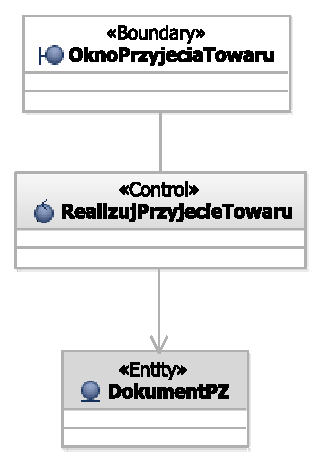
\includegraphics[angle=\ecbangle, scale=\ecbscale]{../img/usecase/pu27ecb.pdf}
  \caption{\ecbcaption27}
\end{figure}

\begin{figure}[H]
  \centering
  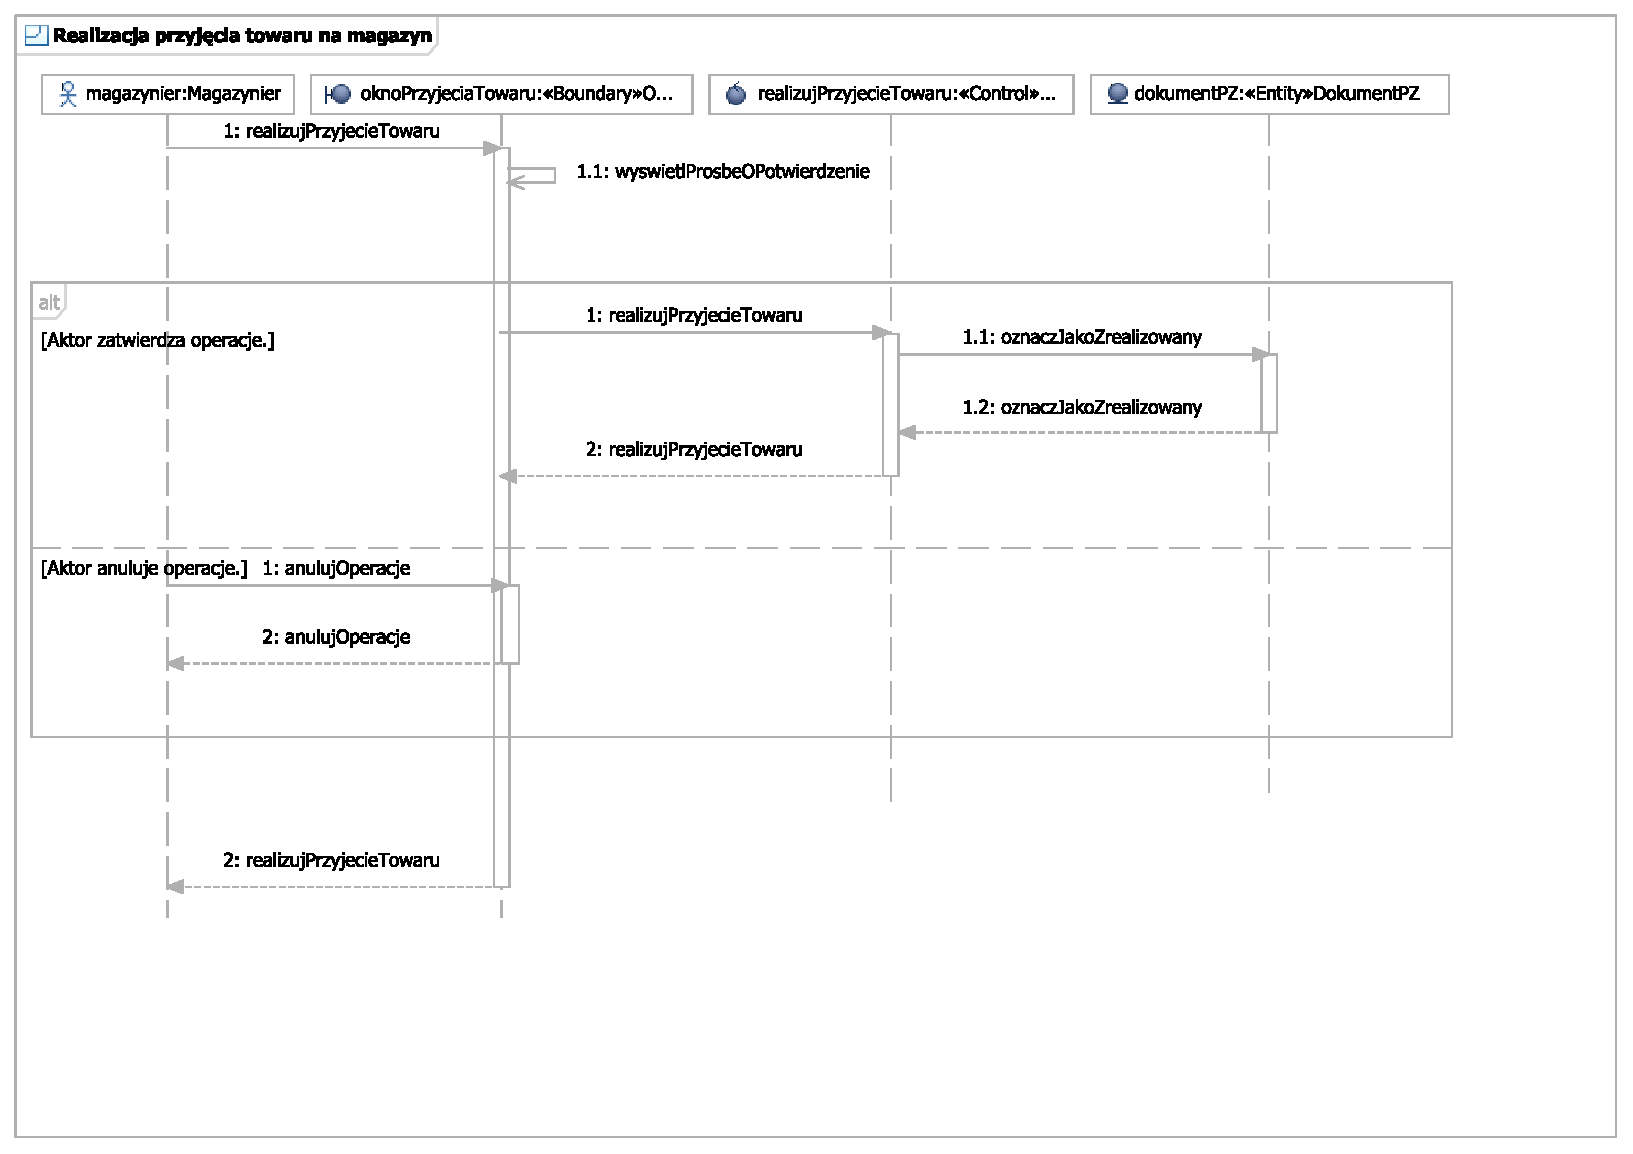
\includegraphics[angle=\seqangle, scale=\seqscale]{../img/usecase/pu27seq.pdf}
  \caption{\seqcaption27}
\end{figure}
\newpage

\subsection{Korekta przyjęcia towaru}
\begin{usecase}
  \addtitle{PU28}{Korekta przyjęcia towaru}
  \addfield{Priorytet:}{wysoki}
  \addfield{Aktor główny:}{Magazynier}
  \addfield{Rozszerza przypadki:}{PU23}
  \additemizedfield{Warunki początkowe:}{
     \item Aktor został uwierzytelniony.
     \item Wybrany dokument przyjęcia towaru został już zrealizowany.
  }
  \additemizedfield{Warunki końcowe:}{ 
    \item Dokument korekty przyjęcia towaru został zapisany w systemie.
    \item Ilość przechowywanych towarów została zaktualizowana zgodnie z wartością podaną na korekcie. 
    \item Ilość przechowywanego towaru jest zgodna z warunkami poprawności danych przedstawionymi w \ref{dziedzina-problemu}.
  }
  \addscenario{Scenariusz główny:}{
    \item Aktor wybiera opcję utworzenia korekty dla wskazanego dokumentu przyjęcia towaru.
    \item System wyświetla formularz nowej korekty. 
    \item Aktor wypełnia podstawowe dane korekty.
    \item Aktor wybiera towary, które podlegają zwrotowi oraz ich cenę.
    \item Aktor wybiera opcję zapisania korekty.
    \item System informuje aktora, że dane zostały poprawnie zaktualizowane.
  }
  \addscenario{Scenariusz alternatywny:} {
    \item [3.a] Aktor nie podał wymaganych pól formularza:
      \begin{enumerate}
        \item[1--4.] Jak w scenariuszu głównym.
        \item[5.] System wyświetla powiadomienie o konieczności podania wymaganych informacji.
        \item[6.] Aktor wraca do punktu 3.  
      \end{enumerate}
    \item [3.b] Aktor podał błędne wartości pól formularza:
      \begin{enumerate}
        \item[1--4.] Jak w scenariuszu głównym.
        \item[5.] System wyświetla powiadomienie o błędnych polach formularza.
        \item[6.] Aktor wraca do punktu 3.
      \end{enumerate}
     \item[5.a] Aktor wybrał ten sam towar co najmniej dwa razy.
       \begin{enumerate}
       \item[1--5.] Jak w scenariuszu głównym.
       \item[6.] System informuje aktora, że co najmniej dwa razy wybrał ten sam towar, podane ilości towaru zostaną więc zsumowane.
       \item[7.] System wyświetla zsumowane wartości dla tych samych towarów.
       \item[8--...] Jak w scenariuszu głównym.
       \end{enumerate}
  }
  \addfield{Zakres przetwarzanych danych:} {
    Pola dokumentu przyjęcia towaru takie jak przedstawione w rozdziale \ref{dziedzina-problemu}.
  }
  \addfield{Warunki poprawności danych:}{
    Warunki poprawności takie jak przedstawione w rozdziale \ref{dziedzina-problemu}.
  }
  \addfield{Wymagania funkcjonalne:}{4.5}
\end{usecase}

\begin{figure}[H]
  \centering
  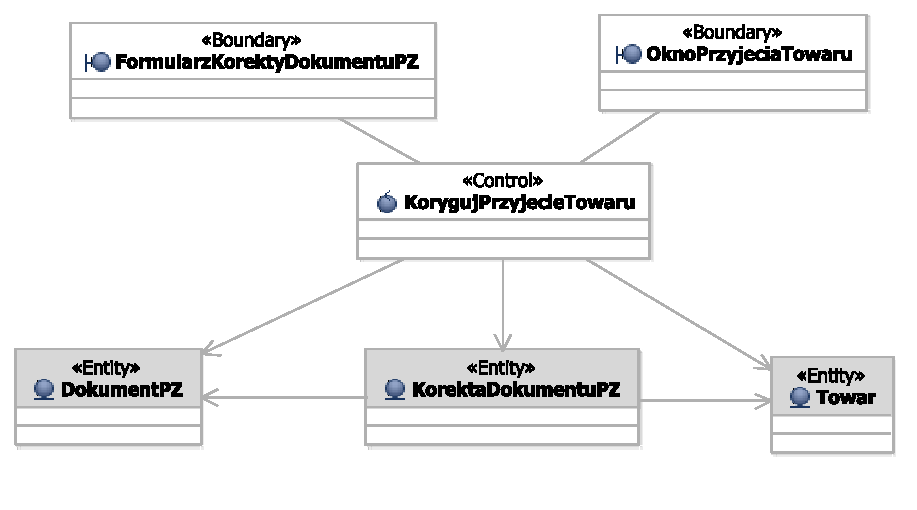
\includegraphics[angle=\ecbangle, scale=\ecbscale]{../img/usecase/pu28ecb.pdf}
  \caption{\ecbcaption28}
\end{figure}
\newpage
\begin{figure}[H]
  \centering
  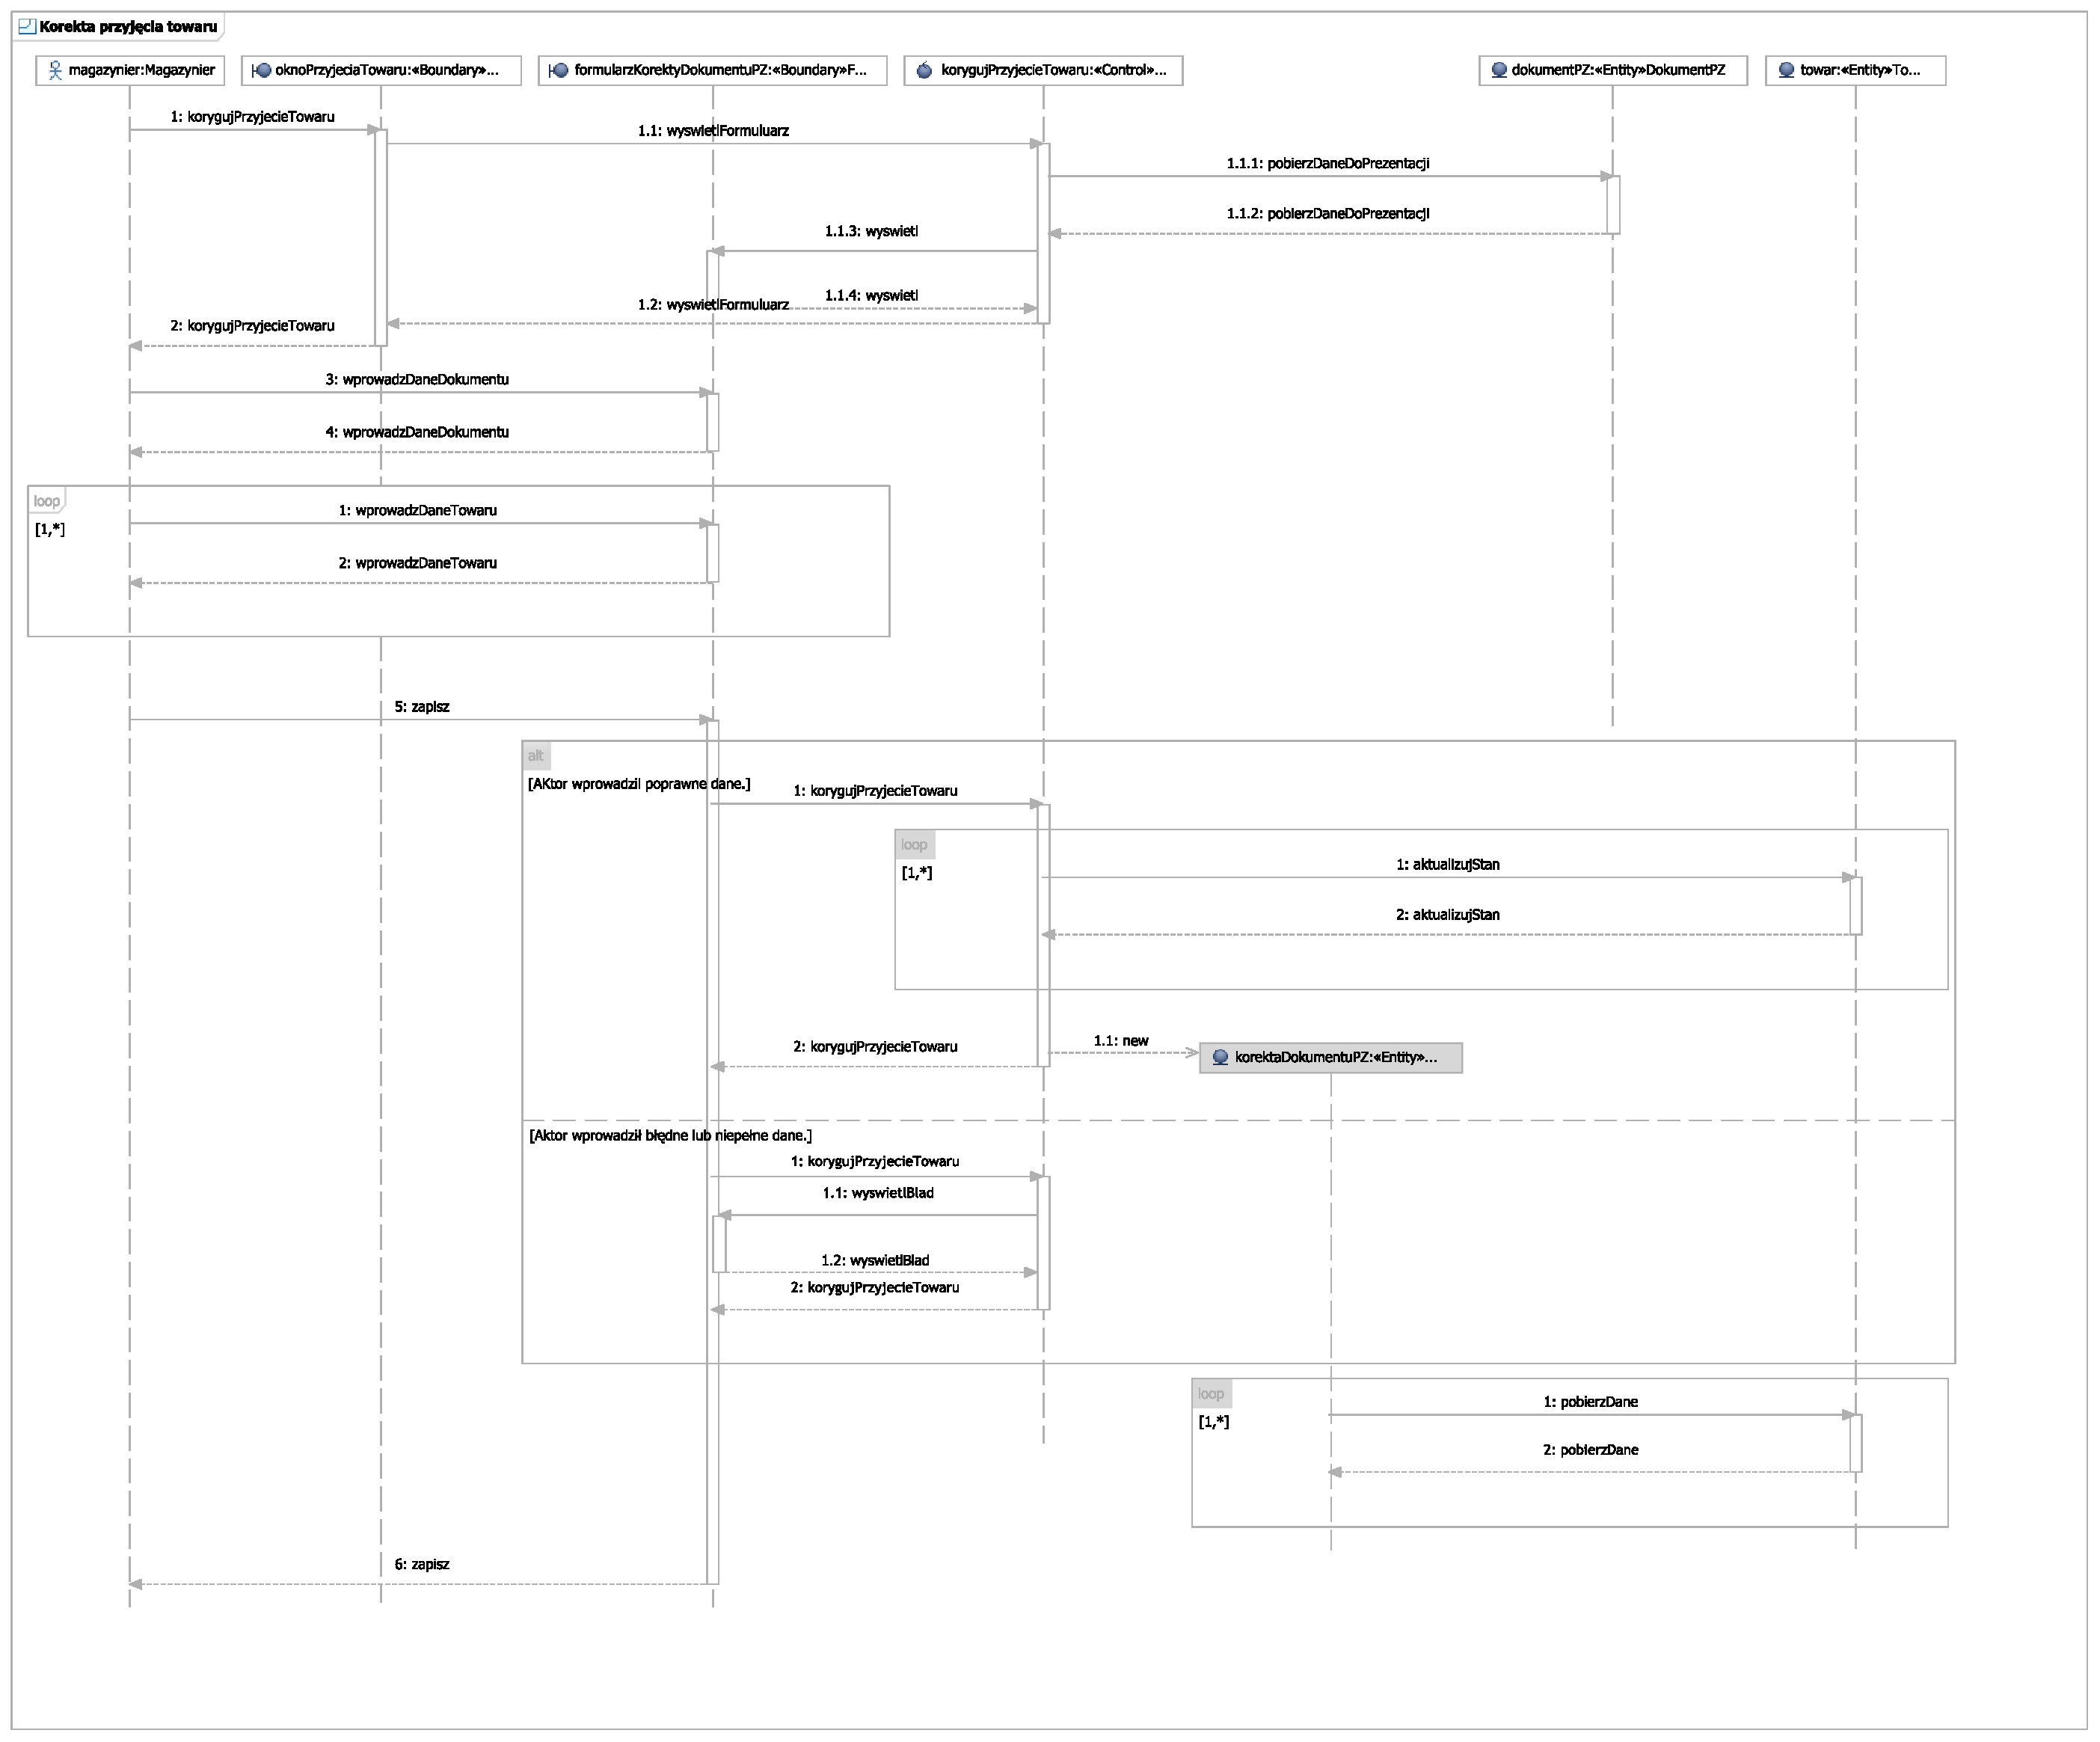
\includegraphics[angle=\seqangle, scale=0.35]{../img/usecase/pu28seq.pdf}
  \caption{\seqcaption28}
\end{figure}
\newpage








\chapter{Model analityczny}
tereferere

\chapter{Wstępna specyfikacja rozwiązania}
terefere


\end{document}
